\documentclass[11pt, a4paper]{book}

\usepackage{svn-multi}
\svnid{$Id$}
\usepackage{prelim2e}

\usepackage{listings}
\lstset{
    frame=single,
    breaklines=true,
    postbreak=\raisebox{0ex}[0ex][0ex]{\ensuremath{\color{red}\hookrightarrow\space}}
}

\usepackage{appendix}
%\usepackage{bookmark}
\usepackage{import}


\renewcommand{\PrelimWords}{Draft Copy \svnkw{Id}}
\newcommand*{\mysvnrev}{\svnrev}
\usepackage[hyperindex=true,
			bookmarks=true,
            pdftitle={Decisions, Learning and Games; You've Got To Have Freedom.}, pdfauthor={Nicol\'as Della Penna},
            colorlinks=false,
            pdfborder=0,
            pagebackref=false,
            citecolor=blue,
            plainpages=false,
            pdfpagelabels,
            pagebackref=true,
            hyperfootnotes=false]{hyperref}
\usepackage[all]{hypcap}
\usepackage[palatino]{anuthesis}
\usepackage{afterpage}
\usepackage{graphicx}
\usepackage{thesis}
\usepackage{epigraph}
\usepackage[square]{natbib}
\usepackage[normalem]{ulem}
\usepackage[table]{xcolor}
\usepackage{makeidx}
\usepackage{cleveref}
\usepackage[centerlast]{caption2}
\usepackage{float}
\urlstyle{sf}
\renewcommand{\sfdefault}{uop}
\usepackage[T1]{fontenc}
\usepackage[scaled]{beramono}

\usepackage{multirow}

\usepackage{tikz}
\usetikzlibrary{positioning}

\renewcommand*{\backref}[1]{}
\renewcommand*{\backrefalt}[4]{
  \ifcase #1 %
    %
  \or
    (cited on page #2)%
  \else
    (cited on pages #2)%
  \fi
}




\usepackage[utf8]{inputenc} % allow utf-8 input
\usepackage[T1]{fontenc}    % use 8-bit T1 fonts
\usepackage{hyperref}       % hyperlinks
\usepackage{url}            % simple URL typesetting
\usepackage{booktabs}       % professional-quality tables
\usepackage{amsfonts}       % blackboard math symbols
\usepackage{nicefrac}       % compact symbols for 1/2, etc.
\usepackage{microtype,natbib}   

\usepackage{times,bbm,amsthm,comment,amssymb,amsmath,amsfonts, mathtools, hhline, enumerate}

\usepackage{subfigure} 
%\usepackage{algorithm,algpseudocode}
%\usepackage{algorithmic}

\usepackage{algorithm}
\usepackage{algorithmic}

\mathtoolsset{
showonlyrefs=true%true % or false in draft mode
}



\DeclareMathOperator*{\argmax}{argmax}
\DeclareMathOperator*{\argmin}{argmin}
\DeclareMathOperator*{\argsup}{argsup}
\DeclareMathOperator*{\arginf}{arginf}
\DeclareMathOperator*{\diag}{diag}

\DeclareMathOperator*{\expec}{\mathbb E}
\DeclareMathOperator*{\exphat}{\hat{\mathbf E}}
\newcommand{\indic}{{\mathbbm 1}}

\newcommand{\chosen}{{\texttt{Chosen}}}
\newcommand{\actual}{{\texttt{Actual}}}
\newcommand{\comply}{{\texttt{Comply}}}

\newcommand{\x}{{\mathbf x}}
\newcommand{\y}{{\mathbf y}}
\newcommand{\wt}{{\mathbf w}}
\newcommand{\vt}{{\mathbf v}}
\newcommand{\bp}{{\mathbf p}}
\newcommand{\bP}{{\mathbf P}}
\newcommand{\bt}{{\mathbf b}}
\newcommand{\be}{{\mathbf e}}
\newcommand{\cA}{{\mathcal A}}
\newcommand{\cB}{{\mathcal B}}
\newcommand{\cC}{{\mathcal C}}
\newcommand{\cH}{{\mathcal H}}
\newcommand{\cR}{{\mathcal R}}
\newcommand{\bR}{{\mathbb R}}

\newcommand{\fN}{{\mathfrak N}}
\newcommand{\fC}{{\mathfrak C}}
\newcommand{\fA}{{\mathfrak A}}
\newcommand{\fD}{{\mathfrak D}}


\newcommand{\grad}{\operatorname{\nabla}}
\newcommand{\dd}{{\partial}}

\newcommand{\prob}{{\mathbb P}}
\newcommand{\probq}{{\mathbb Q}}

\newcommand{\eod}{{${}$\\}}

\newcommand{\regret}{{\mathtt{Regret}}}
\newcommand{\proj}{{\mathtt{Proj}}}

\newcommand*\loss{\ensuremath{\boldsymbol\ell}}
\newcommand*\Loss{\ensuremath{\mathcal L}}
\newcommand*\error{\mathcal E}

\newtheorem{mech}{Mechanism}[chapter]
\newtheorem{thm}{Theorem}[chapter]
\newtheorem{cor}{Corollary}[chapter]
\newtheorem{prop}{Proposition}[chapter]
\newtheorem{lem}{Lemma}[chapter]
\newtheorem{eg}{Example}[chapter]
\newtheorem{defn}{Definition}[chapter]
\newtheorem{assn}{Assumption}[chapter]
%\newtheorem{claim}[thm]{Claim}[chapter]
\theoremstyle{remark}[chapter]
\newtheorem*{idea}{Proof idea}[chapter]
\newtheorem*{rem}{Remark}[chapter]
\newtheorem*{qu}{Question}[chapter]
\newtheorem{conjecture}{Conjecture}[chapter]


            

\title{Decisions, Learning and Games: \\ You've Got To Have Freedom.}
\author{Nicol\'as Della Penna}
\date{\today}

\renewcommand{\thepage}{\roman{page}}

\makeindex
\begin{document}

\pagestyle{empty}
\thispagestyle{empty}
%% anuthesis.sty Copyright (C) 1996, 1997 Steve Blackburn
%% Department of Computer Science, Australian National University
%%

\begin{titlepage}
  \enlargethispage{2cm}
  \begin{center}
    \makeatletter
    \Huge\textbf{\@title} \\[.4cm]
    \Huge\textbf{\thesisqualifier} \\[2.5cm]
    \huge\textbf{\@author} \\[9cm]
    \makeatother
    \LARGE A thesis submitted for the degree of \\
    Doctor of Philosophy  \\
    The Australian National University \\[2cm]
    \thismonth
  \end{center}
\end{titlepage}


\vspace*{14cm}
\begin{center}
  \makeatletter
  \copyright\ \@author{} 2016
  \makeatother
\end{center}
\noindent
\begin{center}
  \footnotesize{~} %\aboutthesis
\end{center}
\noindent

\newpage

\vspace*{7cm}
\begin{center}
  Except where otherwise indicated, this thesis is my own original work.
\end{center}

\vspace*{4cm}

\hspace{8cm}\makeatletter\@author\makeatother\par
\hspace{8cm}\today

\cleardoublepage
\pagestyle{empty}
\vspace*{7cm}
\begin{center}
a Lucia, Laura \& Claudio, por todo.
\end{center}


\cleardoublepage
\pagestyle{empty}
\chapter*{Acknowledgments}
\addcontentsline{toc}{chapter}{Acknowledgments}

Mark D. Reid provided maximal freedom as a supervisor.
Bob Williamson was incredibly patient as chairman.
He and three anonymous reviewers who provided constructive comments that greatly improved this work.  

David Balduzzi was an excellent friend and productive collaborator.
Yiling Chen gave generous advice when I was starting to understand the predictions literature.
Scott Sanner was always thoughtful and methodical in engaging with even my wildest questions and frustrations.


Leo Celi and Rob Stretch where generous in helping me in my attempts to understand decision making in medical practice.
Ben Moran and Adam Kelly, for the friendship and the many conversations that helped me understand the constructive side of contingent claims.

Rafael Frongillo, Brendan van Rooyen, and Garrett Johnson, for their steady and reasonable friendships.
Alice Hutchings, Brendan Loo Gee, Karina Vennonen, Mitchell Jon Brown, Blaine Cook and Natasha Carolan for their incredibly generous hospitality and friendship over these yeas.

Avi Ruderman was an ideal co-conspirator and academic sibling. 
Maja Tampe, Tamar Regev, Jacinta Torres, Dar\'io Garc\'ia Garc\'ia, Carsten Riechelmmann, and Erik Garrison, for the countless decisions in these years that my interactions with them helped improve, and the larger number they graciously accepted despite my unreasonable. 




\cleardoublepage
\pagestyle{headings}
\chapter*{Abstract}
\addcontentsline{toc}{chapter}{Abstract}
\vspace{-1em}


Maintaining subjects freedom to decide imposes structure and constraints on learning systems that aim to guide those decisions. Two natural sources to learn to make good decisions are past experiences and advice from others. Both are affected by subjects freedom to ultimately act as they wish; giving rise to learning theoretic and game theoretic repercussions respectively.

To study the first we extend the standard bandit setting: after the algorithm chooses an action, the subject may actually carry out a different action and then this is observed along with the reward. Algorithms whose choice of action are mediated by a subject can gain from awareness of the subjects' actual actions, which we term compliance awareness. We present algorithms that take advantage of compliance awareness, while maintaining worst case regret bounds up to multiplicative constants.  We study their empirical finite sample performance on synthetic and simulations with real data from clinical trials. Finally we draw connections to a broader machine learning literature on learning with privileged information and generalized distiliation.  
%Where, instead of a compliance variable which maps to the action space, arbitrary variables observed after the action has been chosen by the algorithm can be taken into account.

To study the advice of others, we consider the literature on incentivizing multiple experts by a decision maker that will take an action and receive a reward about which the experts may have information. Existing mechanisms for multiple experts are known not to be truthful, even in the limited sense of myopic incentive compatibility, unless the decision maker renounces their ability to always take on the best ex-post action and commits to a randomized strategy with full support. We present a new class of mechanisms based on second price auctions that maintain subjects freedom. Experts submit their private information, and the algorithm auctions of the rights to a share of the reward of the subject, who then has freedom to pick the action they desire after observing the submitted information. We show several situations in which existing mechanisms fail and this one succeeds. We also consider strategic limitations of this mechanism beyond the myopic setting that arrise due to information complementarities, and practical considerations in its implementation in real institutions.


We conclude by considering a natural hybrid setting, where a sequence of subjects makes decisions and each can receive advice from a fixed set of experts that the mechanism seeks to incentivize. 
The model for this setting is extremely general, having as special cases: standard, compliance aware and contextual bandits, as well as decision markets.
We present a novel market structure that incentivizes exploration, information revelation, and aggregation with selfish experts.


%%% Local Variables: 
%%% mode: latex
%%% TeX-master: "paper"
%%% End: 

%% Table of contents
\cleardoublepage
\pagestyle{headings}
\markboth{Contents}{Contents}
\tableofcontents
\listoffigures
\listoftables

\mainmatter
%!TEX root = main.tex
%%%%%%%%%%%%%%%%%%%%%%%%%%%%%%%%%%%%%%%%%%%%%%%%%%%%%%%%%%%%%%%%%%%%%%%%%%%%%%%%%%%%%%%%
\section{Introduction}
\label{bandintro}

People often don't do as they are told. Approximately 50\% of patients suffering from chronic illness do not take prescribed medications (\cite{sabate:03}). It is safe to assume that the rate at which patients or doctors will follow the recommendations provided by an algorithm will fall well short of 100\%. 
Unfortunately, despite its importance in medical applications (\cite{vrijens:12,hugtenburg:13}), compliance has not been analyzed in the bandit literature. 

In this chapter, we introduce compliance awareness into the \emph{bandit setting} (\cite{bubeck:12}).
Bandit problems are concerned with optimal repeated decision-making in the presence of uncertainty. The main challenge is to trade-off exploration and exploitation, so as to collect enough samples to estimate the rewards from different strategies whilst also strongly biasing samples towards those actions most likely to yield high rewards.  
Our running example is an algorithm that recommends treatments to patients. For concreteness, consider a mobile app that encourages patients who have recently suffered a stroke to carry out various low intensity interventions that may be beneficial in preventing future strokes.
These could be as simple as meditating, going for a walk or taking an aspirin.
The effects of the interventions on the probability of a future stroke may be small. The social benefits of collectively choosing the most effective interventions, however, may be large.
 
There are other settings in which compliance information is available. For example, an algorithm could recommend treatments to doctors. Whether or not the doctor then prescribes the recommended treatment to the patient is extremely informative, since the doctor may make observations and have access to background knowledge that is not available to the algorithm.
A quite different setting is online advertising, where bandit algorithms are extensively applied to recommend which ad to display (\cite{graepel:10,mcmahan:13}). In practice, the recommendations provided by the bandit may not be followed. For example, sales teams often have hand-written rules that override the bandit in certain situations. Alternatively, the algorithm may assign a user to a treatment on their laptop, and when the user is not logged in, expose him to a different treatment on their mobile.
Clearly, the bandit algorithm should be able to learn more efficiently if it is provided  with information about which ads were actually shown.

In the classic multi-armed bandit setting, the player chooses one of $k$-arms on each round and receives a reward( \cite{auer:02b,auer:02}). The player is not told what the reward would have been had it chosen a different arm. The goal is to minimize the cumulative regret over a series of $T$ rounds. In the more general compliance setting, the action chosen by the algorithm is not necessarily the action that is finally carried out, see section~\ref{sec:formal}. Instead, a compliance process mediates between the algorithm's recommendation and the action that is actually taken. Importantly, the compliance process may depend on latent characteristics of the subject of the decision. We focus on the case where the outcome of the compliance process is observable.

Unfortunately, compliance information is a two-edged sword. There are settings where it is useful; but  it can also lead to linear regret. We present sub-linear regret algorithms that incorporate compliance information and provide both worst case regret guarantees that match up to multiplicative constants the standard ones for multi-armed bandits (which we term the chosen strategy). We also show with stylized examples situations where compliance aware algorithms have bounded regret and standard ones do not.


\subsection{Outline}
Section~\ref{sec:noncompliance} introduces the formal compliance setting and introduces three protocols for incorporating compliance information into bandit algorithms. Each protocol has strengths and weaknesses. The simplest protocol ignores compliance information -- yielding the classical setting where standard regret bounds hold. If, instead of attending to its recommendations, the bandit attends to whether the patient actually takes the treatment, then it is possible to learn faster than without compliance information. On the other hand, there are no guarantees on convergence when an algorithm attends purely to the compliance of patients and ignores its own prior recommendations -- examples of linear regret are provided in section~\ref{sec:protocols}. 

A natural goal is thus to simultaneously incorporate compliance information whilst preserving the no-regret guarantees of the classical setting. We then present two hybrid algorithms that do both. The first, \texttt{HB} is in a two-level bandit algorithm. The bottom-level learns three experts that specialize on difference kinds of compliance information. The top-level is another bandit that learns which expert performs optimally. The algorithm thus has no-regret against both the treatments and two natural reward protocols that incorporate compliance information. The second algorithm, \texttt{TB}, rapidly converges to Thompson sampling with standard guarantees. However, when Thompson sampling is unsure about which arm to pull, the algorithm takes advantage of the uncertainty to introduce arm-pulls sampled from \texttt{HierchicalBandit}.

Empirically, \texttt{TB} achieves a surplus of 8.9 extra survivals (that is, human lives) relative to the randomized baseline.
The \texttt{HB} algorithm with \texttt{Epsilon Greedy} as the base algorithm achieves a surplus of 9.2.
In contrast, the best performing strategy that is not compliance aware is Thompson sampling, which yields 7.9 extra survivals.



\subsection{Comparison with other bandit settings}
It is useful to compare noncompliance with other bandit settings. Partial monitoring is concerned with situations where the player only partial observes its loss \cite{alon:15}. Our setting is an extension of the bandit setting, where additional compliance-information is provided. Whether or not a patient complies is a form of side-information. However, in contrast to the side-information available to contextual bandits, compliance is only observed \emph{after} an arm is pulled. An interesting question, left for future work, is how contextual and compliance information can both be incorporated into bandit algorithms.

Hybrid algorithms were previously proposed in the best-of-both-worlds scenario( \cite{bubeck:12a,seldin:14}), where the goal is to construct a bandit that plays optimally in both stochastic and adversarial environments. Vapnik introduced a related notion of side-information into the supervised setting with his learning under privileged information framework (\cite{vapnik:09}). 
An important point of comparison is the bandits with unobserved confounders model introduced in( \cite{bareinboim:15}). That paper was motivated using an extended example involving two subpopulations (drunk and sober) gambling in a casino. Since we are primarily interested in clinical applications, we map their example onto two subpopulations of patients, rich and poor. Suppose that rich patients always take the treatment (since they can afford it) and that they are also healthier in general. Poor patients only take the treatment when prescribed by a doctor.

In \cite{bareinboim:15}) they observe that the question ``what is the patient's expected reward when taking the treatment (formally: $\expec[R|{A=1}]$)?'' is confounded by the latent variable \texttt{wealth}. Estimating the effect of the treatment -- which may differ between poor and rich patients -- requires more refined questions. In our notation: 
``what is the patient's expected reward when taking the treatment, given she is wealthy (formally: $\expec[R|{A=1}, \text{always-taker}]$)?'' and  ``what is the patient's expected reward when taking the treatment, given she is poor (formally: $\expec[R|{A=1}, \text{complier}]$)'', see example~\ref{eg:rich}.
The solution proposed in (\cite{bareinboim:15}) is based on the regret decision criterion (RDC), which estimates the optimal action according to $\argmax_{a}\expec[R|A=a,\text{patient's inclination}]$, where the action chosen, $A=a$, may \emph{differ} from the patient's latent inclination. Essentially, computing the RDC requires imposing interventions via the $do(\cdot)$ operator. However, overruling a patient or doctor's decision is often impossible and/or unethical in clinical settings. The counterfactual information required to compute the RDC may therefore not be available in practice.
Compliance information does not act as a direct substitute for the $do(\cdot)$ operator. However, compliance information is often readily available and, as we show below, can be used to ameliorate the effect of confounders by giving a partial view into the latent structure of the population that the bandit is interacting with.






\chapter{Background and Related Work}
\label{cha:background}

%\epigraph{Desvar\'io laborioso y empobrecedor el de componer vastos libros; el de explayar en quinientas p\'aginas una idea cuya perfecta exposici\'on oral cabe en pocos minutos.{Jorge Luis Borges,Pr\'ologo de Ficciones.}

%Los deterministas niegan que haya en el mundo un solo hecho posible, id est un hecho que pudo acontecer; una moneda simboliza nuestro libre albedrío. (€œEl Zahir€)


We first provide a overview of the game theoretical background that underpins all aspects of this work. The literatures on bandits and decision elicitation have remained largely separate, and the rest of the background section reflects this. 


We search for mechanisms that have good equilibria in the sense of efficiency and truthfulness, where learning dynamics can help arrive on those equilibria. In a sense, dominant strategy and BNE are the limits of purely deductive learning, since the optiomal action can be deduced purely from the sructure of the game before it is played. In the case of the dominant strategies it is robust (in the minimax sense) tot he motivation and information of the other agents, this also limits the degree of efficiency it can achieve. BNE on the other hand, suffer the opposite problem, we will see that is sufficiently rich priors are common knowledge then there are equilibria that are fully revealing, but can be many other equilibria where nothing is learnt; being inherently nonconstructive BNE cant help us distinguish between these. 


\section{Notation and Conventions}


The notation used for is a compromise to accomodate as much as possible the conventions of both the bandit algorithms and mechanism design literatures, while adding the distinction between the action the algorithm or mechanism chooses and the one that the subject actually carries out in the world. We refer to throughout as the \emph{chosen} action and notate as $c$, and the action that the subject takes on the world, which we refer to this as the \emph{actual} action, and notate as $a$).

We follow the bandit literature and refer to rewards as directly observable after the actual action is taken, skipping the the maping of actions to outcomes, and the utility functions which map those outcomes to rewards. The reader wishing to move the analysis more explciitly in the mechansim design tradition can replace the observed rewards with the von Neumann Morgensten utility function of the agent over the realized outcome.
%TODO: spell it out in greek

All models in the later part of the book use finite action spaces, so as to gurantee the existance of nash eqilibria. Since actions involve reports of signals, this contraints all signals to also be discrete. 



\section{Background}


Statistical learning algorithms can be understood game theoretically as a game between a forecaster and nature.This is particularly natural in the sequential (online) setting, and \cite{cesa2006prediction} provide a unified treatment from a worst case game theoretic perspective of many such learning settings and algorithms.
This literature largely consider the underlying structures to be zero-sum and thus use a adversarial model of nature to construct strategies that have good worst case properties. In other words this is game theory in the style of Von Neumann and Morgensten 1948, where minimax is pre-eminent. 

When there are multiple agents beyond nature interacting, as in elicitation from multiple experts for decision making, there are severe limits to what worst case analysis alone can yield. In particular, the notions of nash equilibrium \cite{nash1950equilibrium} and common knowledge \cite{aumann1976agreeing} provide a useful starting point to thinking about equilibria in such settings, through they leave us with an embarrassment of riches in terms of the potetial equilibrium set. Their 


\subsection{Bandits}

Decisions over mutually exclusive actions that affect reward naturally lead to partial supervision.
Bandit problems are concerned with optimal repeated decision-making in the presence of uncertainty and partial supervision, while being simpler than full reinforcement learning in that they limit the underlying state of the system to evolve in a manner indepedent of the set of actions carried out. 
The main challenge is to trade-off exploration and exploitation, so as to collect enough samples to estimate the rewards from different strategies whilst also strongly biasing samples towards those actions most likely to yield high rewards.  

 A well studied example of prediction game is the following is the contextual bandit setting: In each round, nature reveals some context, the adversary privately assigns a loss value to each action in a fixed set.
 Then the player chooses an action (possibly using randomization), incurs the corresponding loss, the player only observes the loss of the chosen action, but not that of other actions.
 The goal of the player is to control static regret, which is defined as the excess loss incurred by the player as compared to the best fixed action given the context over a sequence of rounds.


\subsubsection{Thompson Sampling}

 A very natural algorithm with good practial performance and is first proposed in the literature by \cite{thompson:33}, play each action with probability equal to its posterior probability of being the best action.



% %  The
% % general structure of TS involves the following elements
% % (this description of TS follows closely that of
% % Chapelle and Li [2011]):
% % 1. a set ψ of parameters ˜µ;
% % 2. an assumed prior distribution P(˜µ) on these parameters;
% % 3. past observations D consisting of (reward r) for
% % the arms played in the past time steps;
% % 4. an assumed likelihood function P(r|µ˜), which
% % gives the probability of reward given a context
% % b and a parameter ˜µ;
% % 5. a posterior distribution P(˜µ|D) ∝ P(D|µ˜)P(˜µ),
% % where P(D|µ˜) is the likelihood function.

% % The notation P(·) in above denotes probability density.
% % TS maintains a posterior distribution for the underlying
% % parameter µi
% % , i.e. the expected reward, of every
% % arm i. In each round, TS plays an arm according to
% % its posterior probability of being the best arm, that is,
% % the posterior probability of having the highest value of
% % µi
% % . A simple way to achieve that is to produce a sample
% % from the posterior distribution of every arm, and
% % play the arm that produces the largest sample. Below
% % we describe two versions of TS, using Beta priors
% % and Bernoulli likelihood function,

% and using Gaussian
% % priors and Gaussian likelihood respectively.
% % We emphasize that the Beta priors and Bernoulli likelihood
% % model, or Gaussian priors and the Gaussian likelihood
% % model for rewards are only used below to design
% % the Thompson Sampling algorithm. Our analysis of
% % these algorithms allows these models to be completely
% % unrelated to the actual reward distribution. The assumptions
% % on the actual reward distribution are only
% % those mentioned in Section 1.1, i.e., the rewards are in
% % the range [0, 1]. I



\subsubsection{Beyond IID and Static Regret: Exp3}

 Maximally robust guarantees, in particular wrt non-stochastic nature of underlying sequences. Useful when we wish to create hierarchical bandits when the original sequence may not be IID, the sequence that results from a bandits algorithms choices will not be by construnction.



\subsection{Information Design and Incentive Compatible Bandits}

% Information Design, Bayesian Persuasion, and Bayes Correlated Equilibrium,  American Economic Review Papers and Proceedings, 2016, 106, 586-591, with Stephen Morris


 \cite{mansour2015bayesian}


% complexity theory of algorithmic persuasion
%http://arxiv.org/pdf/1503.05988.pdf



\subsection{Information Aggregation and Incentives}

A literature in economics and particularly mechanism design, is centered on when and how information can be aggregated from multiple agents that receiv signals about the state of the world, and have various degrees of strategic sophistication in their actions.



% % THERE EXISTS AN EXTENSIVE LITERATURE on efficient auctions and mechanism
% % design. A lot of attention has been devoted to the case where each agent i has a
% % quasi-linear utility function that depends on the chosen social alternative, on
% % information or signal privately known to  . i, and on a monetary transfer, but
% % does not depend on information available to other agents. In this framework, a
% % prominent role is played by the Clarke-Groves-Vickrey CGV mechanisms see 
% % Clark 1971 , Groves 1973 , Vickrey 1961 . These are mechanisms that ensure 
% % both that an efficient decision is taken and that truthful revelation of privately
% % held information is a dominant strategy for each agent.
% %  The result holds for
% % %arbitrary dimensions of signal spaces and for arbitrary signals€™ distributions.
% % In this paper we study the case where each agent has a quasi-linear utility
% % function having as arguments signals received by all agents and the chosen
% % social alternative. Hence, besides allocative externalities, we allow for informational
% % %externalities, and we speak of €˜interdependent valuations. Signals may
% % be multi-dimensional, but we assume that they are independently drawn across
% % agents. Signal independence is the most seriously restrictive assumption;}


\subsubsection{Prediction Markets} 

The closest contact point between the online learning and information elicitation literatures is in the fully supervised case.
That is the information the market is attempting to aggregate is a forecast of the future state of the world that is not contigent on the actions that can be influencd by it. Thus, at the time of realization of the event, we can judge not only the forecast obtained but also any other potential forecast that ould have been received. 
This contrasts this with the bandit setting, where instead of a forecast of the state of the world we seek an action that results in a state of the world that is maximally beneficial.  



The equivalence between trading shares and eliciting beliefs from a single agent by the means of scoring rules goes back at least to \cite{savage1971elicitation}. 
%Hanson (2003), Pennock (2006), and Chen and Pennock (2007) discussed this cor- respondence for the case of MSR. The study of automated market makers goes back to Black (1971a, 1971b), while formal analysis of inventory-based market makers goes back to Amihud and Mendelson (1980).



% %The correspondence between trading shares and eliciting beliefs from a single agent by the means of scoring rules was first noted by Savage (1971), who also provided additional techni- cal details. 
% %

% %Under the basic MSR (introduced by Hanson (2003, 2007), though the idea of repeatedly using a proper scoring rule to help forecasters aggregate infor- mation goes back to McKelvey and Page (1990))
% \cite{mckelvey1990public}
% %Note also that if each player behaves myopically in each period, the prediction that he will make is his posterior belief about the expected value of the security, given his initial information and the history of revisions up to that point, and thus the €œgame€ turns into the communication process of Geanakoplos and Polemarchakis (1982).

Initiating with the equivalence between market scoring rules and regularized follow the leader algorithms in \cite{chen2010new} and series of follow up works \cite{abernethy2013efficient, frongillo2012interpreting, hu2014multi, frongillo2015convergence,} that map prediction markets to learning algorithms. 

Subjects freedom makes no difference in the analysis of these fully supervised setting; since there is no action to take, there is no sense in which a subject may not follow along. To the degree the information they surface is not being used strategically by the agents, we can perfectly evaluate how accurate they are regardless of the other agents reports.
% note this is not the case in our ex-comp one shot example, where to evaluate one experts acuracy we need the truthful signal from the other 




%This assumption seems to largely have held for sports and politics, and betting markets over both 

Another notable difference between the decision and 




\subsubsection{Decision Markets}

Contracts that pay if a publicly verifable event occurs are generally regulated as effectively gambling,  severely restricts their use. 

A small  niche of providers of automated market making software for private (particularly corporate outcomes)


 
\cite{berg2003prediction,hanson2002decision,othman2010decision,boutilier2012eliciting,chen2014eliciting}

% \subsection{Decision Markets}

% % \quote{Prediction markets have served as a reliable tool for estimating the winners of political elections and sports games [Berg et al., 2001]. However, due to legal restrictions severely limiting their use, the latest wave of prediction markets have focused not on the general, but on the specific. Instead of creating large-scale markets
% % on publicly verifiable events, these services bill themselves as accu- mulators of organizational knowledge on specific internal (e.g., cor- porate) events. For instance, the prediction 
% % %market startup Inkling Markets suggests that companies use their service €œto uncover and quantify risk in your organization". The recently launched Crowd- cast lists questions like €œWhen will your product really ship?" and €œHow much will it really cost?" on their homepage.
% % We contend that the current corporate prediction markets do not actually capture the problems most prominent for their clients. The chief challenge facing businesses is not whether the decisions they have made will prove successful, but rather what actions to take to assure the best chance of success.
% % %Our work approaches this issue directly. In our model, a princi- pal has to choose an action from a set of possibilities (e.g., €œHire additional sales staff", €œDouble R&D funding") in order to maxi- mize the probability of achieving a desirable outcome (e.g., €œBe- come the top-grossing company in our market space", €œSell more than a million widgets", or €œAchieve profitability by the end of the year"). The principal elicits from an expert, for each action, the probability of achieving the desired outcome. Based on those prob- abilities, the principal then (deterministically) chooses an action ac- cording to a decision rule. Upon success or failure in achieving the desired outcome, the principal rewards the expert according to a pre-determined scoring rule. Three functions define the space: the decision rule, the payoff for success, and the payoff for failure.
% % We first prove general properties of the way these functions re- late. We then provide an in-depth study of the most natural de- terministic decision rule, the max decision rule, which selects the action that has the highest reported success probability. For the single-agent setting, we show that no symmetric scoring rule, nor the asymmetric ones from the literature, give the agent the right in- centives. We construct an asymmetric scoring rule that does, and provide a characterization of a space of such rules.
% % Along the same lines as the original construction of market scor- ing rules [Hanson, 2003, 2007, Pennock and Sami, 2007], we con- tinue by attempting to expand our scoring rule system into an auto- mated market maker for our multiagent setting, to create decision markets. Surprisingly, we show that every market of this kind suf- fers from a peculiar type of manipulability, where an agent benefits from exaggerating the success probability of a suboptimal action. We show that this kind of manipulability applies even under an in- finite stream 
% % %of self-interested agents visiting the market€”even if each agent€™s beliefs about the probabilities are exactly accurate. We design families of asymptotically-optimal pricing rules for decision markets that minimize manipulability.
% % Finally, we study two alternate decision market designs. We show the first one suffers from significant manipulability of a dif- ferent kind, and for the second we show a new kind of no-trade result. 	
% % We initiated the study of decision rules and decision markets in settings where a principal needs to select an action and is advised by a self-interested but decision-agnostic expert about the success probabilities of alternative actions.
% % %We began by investigating the properties of general deterministic decision rules in the context of eliciting from a single expert. We proved results about the relations between the principal€™s decision rule and the rules that specify the expert€™s payoff if the desired out- come is, and is not, achieved. For the most natural decision rule (where the principal takes the action with highest success probabil- ity), we showed that no symmetric scoring rule, nor any of Win- kler€™s asymmetric scoring rules, are quasi-strictly proper. We char- acterized the set of differentiable quasi-strictly proper scoring rules and constructed an asymmetric scoring rule that is quasi-strictly proper.
% % Moving to decision markets where multiple experts interact by trading, we showed a surprising impossibility for every automated market maker, where an agent is incentivized to artificially raise the price of a non-optimal action (again under the decision rule where the principal takes the action with highest success probability). To counter this impossibility, we constructed two families of asymp- totically optimal pricing rules against this form of manipulation, one additively optimal and the other multiplicatively optimal. Fi- nally, we considered two alternative market designs for decision markets. The first, in which all outcomes live in the same proba- bility universe, has even worse incentives (for the final participant). The second, in which the experts trade on the probability of the outcome occurring unconditionally, exhibits a new kind of no-trade result.
% % There are many interesting research directions in this new area.
% % The first would be examining the space of discontinuous scoring rules, being aware that such rules would nevertheless have to obey Theorem 2. Another area of exploration would be combinatorial decision rules, in which the principal could take more than one of the available actions.
% % We focused on deterministic decision rules because they are nat-
% % ural. It is known that adding randomness can significantly increase
% % %the incentive-compatible feasible space of mechanisms in other settings€” prominent examples include voting [Gibbard, 1977] and sybill-proof (false name resistant) voting [Wagman and Conitzer, 2008]. Future research should study randomized decision rules in our setting as
% % %well. Trivial randomized solutions €”like shifting probability to
% % %each action do not get around our impossibilities, like the nonex- istence of strictly proper scoring rules (because the manipulations
% % in our examples and proofs yield the manipulator benefits that are
% % not infinitesimally small).
% % It would also be interesting to explore a larger characterization of the peculiar no-trade impossibility of Section 3.4.2. Does it apply in other economic interactions besides markets of this sort? The key seems to be that any action an agent takes has negative utility because of the effects of taking that action.
% % %Another important direction concerns what happens when agents are interested in the action taken by the principal. For instance, an expert could advocate doubling a company€™s advertising bud- get because she works in the marketing department. This type of setting is related to recent work by Shi et al. [2009], who study a setting where an agent can perform an action after a market runs such that the market can incentivize the agent to act counter to the principal€™s goal. Whether or not the agents can take actions after the decision market, it would desirable to use decision markets to balance the utilities of agents impacted by the principal€™s decision with the principal€™s desire to achieve his goal.}






\section{Related Work}





%A. Kolotilin. Experimental design to persuade. UNSW Australian School of Business Research Paper,


There is to be best of our knowledge no work that previously considers incentives for experts who provide the contextual variables in a contextual bandit problem. Beyond the already mentioned examples of considering the incentives for subjects in bandits, there is little work that brings incentives into the learning with expert advice setting. 


The finl chapters concern with a sequence of decisions, related to this are the properties of repeating one shot seccond price auctions, which has been previously analized in terms of the composability of auctions. 

% Smooth Games, Price of Anarchy and
% Composability of Auctions - a Quick Tutorial
% Abhishek Sinha
% Laboratory for Information and Decision Systems, Massachusetts Institute of Technology, Cambridge, MA 02139
% Email: sinhaa@mit.edu
% Abstract
% In this tutorial we review the concept of smooth games as introduced by Roughgarden in [1]. We show how to upper bound
% the Price of Anrchy of different games using this general tool. Then along the lines of [2], we extend the idea of smooth games
% to smooth mechanisms and weakly smooth mechanisms and prove that many of the common auctions fall under this category. We
% then show how efficiency results of these mechanisms in a Bayes-Nash equilibria may be derived from smoothness arguments.
% Then we prove that simultaneous composition of smooth mechanism preserves the smoothness property. Hence all the previous
% results about efficiency of smooth mechanisms carry over to simultaneous compositions.




% \subsubsection{Efficiency}
% Taken from 
% % \quote{
% % EFFICIENT DESIGN WITH INTERDEPENDENT VALUATIONS
% % BY PHILIPPE JEHIEL AND BENNY MOLDOVANU1
% % We study efficient, Bayes-Nash incentive compatible mechanisms in a social choice
% % setting that allows for informational and allocative externalities. We show that such
% % mechanisms exist only if a congruence condition relating private and social rates of
% % information substitution is satisfied. If signals are multi-dimensional, the congruence
% % condition is determined by an integrability constraint, and it can hold only in nongeneric
% % cases where values are private or a certain symmetry assumption holds. If signals are
% % one-dimensional, the congruence condition reduces to a monotonicity constraint and it
% % can be generically satisfied. We apply the results to the study of multi-object auctions, and
% % we discuss why such auctions cannot be reduced to one-dimensional models without loss
% % of generality.


% % THERE EXISTS AN EXTENSIVE LITERATURE on efficient auctions and mechanism
% % design. A lot of attention has been devoted to the case where each agent i has a
% % quasi-linear utility function that depends on the chosen social alternative, on
% % information or signal privately known to  . i, and on a monetary transfer, but
% % does not depend on information available to other agents. In this framework, a
% % prominent role is played by the Clarke-Groves-Vickrey CGV mechanisms see 
% % Clark 1971 , Groves 1973 , Vickrey 1961 . These are mechanisms that ensure 
% % both that an efficient decision is taken and that truthful revelation of privately
% % held information is a dominant strategy for each agent.
% %  The result holds for
% % %arbitrary dimensions of signal spaces and for arbitrary signals€™ distributions.
% % In this paper we study the case where each agent has a quasi-linear utility
% % function having as arguments signals received by all agents and the chosen
% % social alternative. Hence, besides allocative externalities, we allow for informational
% % %externalities, and we speak of €˜interdependent valuations. Signals may
% % be multi-dimensional, but we assume that they are independently drawn across
% % agents. Signal independence is the most seriously restrictive assumption;}


% The proof of Theorem 4.3 is based on the following technical observation: an
% incentive compatible mechanism generates for each agent a vector field. This
% field associates to each type a vector of expected probabilities with which the
% various alternatives are chosen. A generalization of the standard one-dimensional
% envelope argument shows that this vector field is the gradient of the
% equilibrium expected utility function. Since it is a gradient, the vector field must
% satisfy an integrability condition involving its cross-derivatives.11 The impossibility
% results follow by showing that the vector fields generated by efficient
% mechanisms satisfy the required conditions only under very restrictive conditions.
% Since the integrability constraint bites in any multi-dimensional model, results
% similar to Theorem 4.3 hold as soon as there is at least one agent whose signal is
% of dimension d2.
% In Section 5 we study the remaining case where signal spaces are one-dimensional.
% We construct a mechanism that is efficient and incentive compatible if
% several inequalities relating private and social marginal valuations are satisfied.
% The main idea of the construction is to make i’s transfer equal to the cumulative
% Ž . 12 effect of i’s action here a signal report on all other agents. Since i’s effect on
% others depends here on i’s signal, incentive compatible transfers must neutralize
% this influence.


% \subsection{Information Revelation and Aggregation in Markets}
% TODO: rewrite 
% %\quote{The question of information revelation and aggregation in markets has attracted the attention of many economists, beginning with Hayek (1945). Grossman (1976) formally %showed that in a market equilibrium, the result- ing price aggregates information dispersed among n-types of informed traders, each of whom gets a €œpiece of information.€ In his model, individual traders are small relative to the market, strategic foundations for players€™ behavior are lacking, and the results rely on particular functional forms (e.g., i.i.d. normal errors in signals received by the players; normal prior; etc.). Radner (1979) introduced the concept of Rational Expectations Equilibrium (REE) and showed that generically, a fully revealing REE exists, with prices aggre- gating all information dispersed among traders. Radner€™s paper, however, also lacks strategic foundations. A series of papers explored the question of con- vergence to REE in various dynamic processes (see, e.g., Hellwig (1982), and Dubey, Geanakoplos, and Shubik (1987), for models of centralized trading; Wolinsky (1990), and Golosov, Lorenzoni, and Tsyvinski (2011), for models of decentralized trading; and McKelvey and Page (1986), and Nielsen, Bran- denburger, Geanakoplos, McKelvey, and Page (1990), for models that extend the basic communication process of Geanakoplos and Polemarchakis (1982) to more complex settings in which agents€™ beliefs are iteratively updated in re- sponse to repeated public observations of summary statistics of their actions). In all of these papers, however, it is assumed that each trader ignores the ef- fect of his behavior on the evolution of the trading process, as a result behaving non-strategically along at least one dimension. P

% % roper strategic foundations for the concept of perfect competition with differentially informed agents are offered by the stream of literature studying bidding behavior in single and double auctions (Wilson (1977), Milgrom (1981), Pesendorfer and Swinkels (1997), Kremer (2002), Reny and Perry (2006)). Information aggregation results in these papers, however, rely on the assumption that the market is large, that is, the number of bidders goes to infinity and individual traders become small relative to the market. They also rely on various symmetry assumptions. No such assumptions are made in the current paper, and the number of traders is finite and fixed.

% % Kyle (1985) offered a model of dynamic insider trading, in which the single informed trader takes into account the nonnegligible impact of his actions on market prices. In the continuous version of the model, as time approaches the end of the trading interval, the price of the traded security converges to its true value known by the insider. Foster and Viswanathan (1996) and Back, Cao, and Willard (2000) extended the model to the case of multiple, differentially informed strategic traders. In the continuous case, the price of the traded secu- rity converges to its 
% %expected value conditional on the traders€™ pooled informa- tion. In the discrete case with a finite number of trading periods, convergence is approximate. These models rely on very special functional form assumptions (symmetry, normality, etc.), which allow the authors to construct explicit for- mulas for particular (€œlinear€) equilibria. Laffont and Maskin (1990) criticized this reliance of the results of Kyle (1985) on linear trading strategies; argued that such models inherently have multiple equilibria; presented a model of a trading game with a single informed trader and multiple equilibria, in some of which the informed trader€™s information is not revealed; and concluded that €œin a model in which private information is possessed by a trader who is big enough to affect prices, the information efficiency of prices breaks down€ and €œthe efficient market hypothesis may well fail if there is imperfect competi- tion.€ The results of the current paper show that the conclusions of Kyle (1985), Foster and Viswanathan (1996), and Back, Cao, and Willard (2000) regarding the convergence of the price of a security to its expected value conditional on the traders€™ pooled information do not, in fact, depend on the specific func- tional form assumptions or on the choice of equilibrium: if the traded security is separable, its price converges to its expected value conditional on the pooled information in every equilibrium. In the case of a single informed trader, as in Laffont and Maskin (1990), every security is separable, and so information always gets aggregated. The contrasting conclusions of Laffont and Maskin are thus driven by the specifics of their model, not by the fact that they explicitly consider multiple equilibria. In the case of multiple partially informed traders, the securities considered in Foster and Viswanathan (1996) and Back, Cao, and Willard (2000) have payoffs that are linear in traders€™ signals, and so, as the results of this paper show, information about such securities always gets aggregated as well.

% % This model is based on the market scoring rule (MSR) of Hanson (2003, 2007). In MSR games, there are no noise or liquidity traders and no strategic market makers; the only players are the strategic par- tially informed traders. There is also an automated market maker. This mar- ket maker, in expectation, loses money (though at most a finite, ex ante known amount), %facilitating trade and price discovery. (Without a €œsource€ of prof- its, there would be no trading; see Milgrom and Stokey (1982) and Sebenius and Geanakoplos (1983).) Trading 
% % proceeds as follows. The uninformed mar- ket maker makes an initial, publicly observed prediction about the value of a security. The first informed strategic player can revise that number and make his own prediction, which is also observed by everyone. Then the second player can further modify the prediction, and so on until the last player, after which the first player can again modify the prediction, and the cycle repeats an infinite number of times. The fact that there is an infinite number of trading periods does not mean that the game never ends. %Rather, it is a convenient discrete analogue of continuous trading, with trades taking place at times t0 < t1 < · · · in a bounded time interval. Sometime after the trading is over, the true value of the security is revealed, and each prediction is evaluated according to a strictly proper scoring rule s (e.g., under the quadratic scoring rule, each prediction is penalized by the square of its error; see Section 2.2 for further details). The payoff of a player from each revision is the difference between the score of his prediction and the score of the previous prediction€”in essence, the player €œbuys out€ the previous prediction and replaces it with his own. The total pay- off of a player in the game is the sum of payoffs from all his revisions. Players are risk-neutral. The discounted MSR (Dimitrov and Sami (2008)) is similar, except that the total payoff of a player is equal to the discounted sum of pay- offs from all his revisions, where the payoff from a revision made at time $t_k$ is multiplied by $I^2k$ for some $ i< 1$.
% % While my primary reason for studying this model is to illustrate the intu- ition behind information aggregation in the main model and thus make that result more transparent, information aggregation in MSR-based models is also of independent interest, for several reasons. First, such models can be viewed as generalizations of the communication processes of Geanakoplos and Pole- marchakis (1982) and other papers in this tradition, in which several differen- tially informed agents sequentially announce their beliefs about the value of a random variable (or the probability of an event), and those beliefs eventually
% % converge to a common posterior. In those papers, it is assumed that the agents make truthful announcements, and strategic issues are ignored. Discounted MSR includes this truthful process as a special case, I= 0 (strictly speaking, the case I = 0 is ruled out in this paper, but it is easy to show that as I becomes small, in any equilibrium, players will behave almost %myopically, i.e., will reveal their expectations almost truthfully), and at the same time makes it possible to examine the role of strategic behavior (for β > 0). The results of this paper show that, for separable securities, information aggregation does not depend on whether agents behave strategically or myopically.
% % Second, the MSR model includes as a special case a basic model of trading
% % with an automated inventory-based market maker who offers to buy or sell
% % shares in the security at price p that is a function of the (possibly negative) net
% % inventory the market maker holds at that moment. Specifically, suppose the
% % market maker starts with zero net inventory, sets the price for the security as
% % a continuous decreasing function p(z), where z is the total amount of shares
% % he holds in his inventory (i.e., the more he holds, the less he is willing to pay
% % for additional shares), and commits to buying or selling shares according to
% % that price schedule. Thus, if his current inventory is z0, and a trader decides
% % %to sell (z ˆ’ z ) units of the security to the market maker, the market maker 1 0 ô°‹z1
% % %will pay that trader z0 p(z ̃)dz ̃ for the (z1 ˆ’z0) units. The current price of the security will move from p(z0) to p(z1). If the true value of the security then
% %turns out to be equal to x, then the trader€™s payoff from this transaction will be equal to ô°‹ z1 p(z ̃) dz ̃ ˆ’ x(z1 ˆ’ z0) = ô°‹ z1 (p(z ̃) ˆ’ x) dz ̃ô°· Thus, it is strictly optimal
% %z0 z0
% %(myopically) for the trader to pick z1 in such a way that p(z1) is equal to his
% %belief about the value of the security (assuming the image of function p(·)
% %includes that value). His payoff from this transaction is equal to his payoff from
% s%coring rule s(yô°¸x)= 0 (p(z ̃)ˆ’x)dz ̃, where zy =pˆ’1(y), that is, p(zy)=y.2 Finally, note that while the market maker in this setting expects to lose money, the worst possible loss is bounded and can be controlled by adjusting the parameters of the rule. Another attractive feature of MSR in practice (rel- ative to, say, continuous double auctions) is that a player can instantaneously make his prediction/trade at any time, without having to wait for another player who is willing to take the other side of the trade or to submit a limit order and wait for it to be filled. These features make MSR attractive for use in internal corporate prediction markets, and it is in fact used for that purpose: compa- nies like Consensus Point and Inkling Markets operate MSR-based prediction
% % markets for Ford, Chevron, Best Buy, General Electric, and many other large corporations.3 Thus, the question of whether information in MSR-based pre- diction markets gets aggregated has direct practical implications.
% % Two recent papers have studied the equilibrium behavior of traders in MSR games.4 Chen, Reeves, Pennock, Hanson, Fortnow, and Gonen (2007) consid- ered undiscounted %games based on a particular scoring rule€”logarithmic (see Section 2.2). In their model, the security can take one of two different values, and the number of revisions is finite. They found that if traders€™ signals are in- dependent conditional on the value of the security, then it is an equilibrium for each trader in each period to behave myopically, that is, to make the predic- tion equal to his posterior belief. They also provided an example of a market in which signals are not conditionally independent and one of the traders has an incentive to behave non-myopically. Dimitrov and Sami (2008) also considered games based on the logarithmic scoring rule. In their models, in contrast to Chen et al., traders observe independent signals. Each realization of the vector of signals corresponds to a particular value of the security. The number of trad- ing periods is infinite. Dimitrov and Sami found that, in that case, in the MSR game with no discounting, myopic behavior is generically not an equilibrium and, moreover, there is no equilibrium in which all uncertainty is guaranteed to get resolved after a finite number of periods. They then introduced a two- player, two-signal MSR game with discounting, and proved that in that game, information gets aggregated in the limit, under the additional assumption that the €œcomplementarity bound€ of the security is positive. They reported that, based on their sample configurations, the bound is not always zero, but did not provide any sufficient conditions for it to be positive. In contrast to Chen et al. (2007) and Dimitrov and Sami (2008), the current paper€™s information aggregation results (1) do not rely on the independence or conditional inde- pendence of signals, allowing instead for general information structures with any number of players; (2) do not depend on discounting; and (3) provide a sharp characterization of securities for which information always gets aggre- gated and those for which, under some priors, price may not converge to the expected value conditional on the traders€™ pooled information.}

% %Ostrovsky studies information aggregation in dynamic markets with a finite number of partially informed strategic traders. It shows that, for a broad class of securities, information in such markets always gets aggregated. Trading takes place in a bounded time interval, and in every equilibrium, as time approaches the end of the interval, the market price of a €œseparable€ security converges in probability to its expected value conditional on the traders€™ pooled information. If the security is €œnon-separable,€ then there exists a common prior over the states of the world and an equilibrium such that information does not get aggregated. The class of separable securities includes, among others, Arrow€“Debreu securities, whose value is 1 in one state of the world and 0 in all others, and €œadditive€ securities, whose value can be interpreted as the sum of traders€™ signals.

% %Consider the following example from Geanakoplos and Polemarchakis (1982).
% %EXAMPLE1: Therearetwoagents,1and2,andfourstatesoftheworld,Ω=
% %{Aô°¸Bô°¸Cô°¸D}. The prior is P(ω) = 1 for every ω ˆˆ Ω. The security is X(A) = 4
% %X(D) = 1 and X(B) = X(C) = ˆ’1. Partitions are Π1 = {{Aô°¸B}ô°¸{Cô°¸D}} and Π2 ={{Aô°¸C}ô°¸{Bô°¸D}}.

% %In the example, by construction, it is common knowledge that each player€™s expectation of the value of the security is zero, even though it is also common knowledge that the actual value of the security is not zero, and that the traders€™ pooled information would be sufficient to determine the security€™s value. Thus, even if the traders repeatedly and truthfully announce their posteriors, as in Geanakoplos and Polemarchakis (1982), they will never learn the true value of the security. 




% %\subsection{Extensions}



% \subsubsection{Beyond Partial or Full Supervision}

% Partial observability graph Allows interpolation between full supervision and bandit feedback, shows sharp separations into three classes. 

% When we generalize the notion of compliance-awareness to general awareness of variables 

% Vapnik introduced a related notion of side-information into the supervised setting with his learning under privileged information framework \cite{vapnik:09}.

% Priviledged Information and Generalized Distilation
%  \cite{Lopez-Paz16} show a generalization of distillation, which captures 


% \subsection{Decisions}

% \quote{If we relax the need to elicit probabilities, the problem can be solved straightforwardly. For instance, it is trivial to incentivize an agent to truthfully report which action has the highest probability of achieving a desired outcome. This can be done by simply giving the agent a lump sum payment if the outcome is reached, which aligns the incentives of the agent and the principal.} \cite{othman2010decision}





% \cite{dreber2015using}
% use a prediction market to estimate the reproducibility of scientific research


% a incromprehensible paper, but it is a trivial corolary of the folk theorem (TODO: cites beyond Della Penna and Reid 2012, Chen and ) is that any mechanism that settles before the event occurs has the multiple equilibria. Further if one agent has larger cpaital than the others he can force the settlement to favor him (you might be right, but he is more liquid) %http://bjll.org/index.php/jpm/article/view/1148


% \section{}
% % %http://arxiv.org/pdf/1507.00407v5.pdf
% % It is natural in this setting for the players to each make use of a no-regret learning algorithm for making
% % their decisions, an approach known as decentralized no-regret dynamics. No-regret algorithms
% % are a strong match for playing games because their regret bounds hold even in adversarial environments.
% % As a benefit, these bounds ensure that each player’s utility approaches optimality. When
% % played against one another, it can also be shown that the sum of utilities approaches an approximate
% % optimum [2, 19], and the player strategies converge to an equilibrium under appropriate conditions
% % [7, 1, 9], at rates governed by the regret bounds. Well-known families of no-regret algorithms
% % include multiplicative-weights [14, 8], Mirror Descent [15], and Follow the Regularized/Perturbed
% % Leader [13]. (See [3, 21] for excellent overviews.) For all of these, the average regret vanishes at
% % the worst-case rate of O(1/
% % √
% % T), which is unimprovable in fully adversarial scenarios.
% % However, the players in our setting are facing other similar, predictable no-regret learning algorithms,
% % a chink that hints at the possibility of improved convergence rates for such dynamics. This
% % was first observed and exploited by Daskalakis et al. [4]. For two-player zero-sum games, they developed
% % a decentralized variant of Nesterov’s accelerated saddle point algorithm [16] and showed
% % that each player’s average regret converges at the remarkable rate of O(1/T). Although the resulting

% % We consider the setting where the game G is played repeatedly for T time steps. At each time
% % step t each player i picks a mixed strategy wt
% % i ∈ ∆(Si). At the end of the iteration each player i
% % observes the expected utility he would have received had he played any possible strategy x ∈ Si
% % .
% % More formally, let u
% % t
% % i,x = Es−i∼wt
% % −i
% % [ui(x, s−i)], where s−i
% % is the set of strategies of all but the i
% % th
% % player, and let u
% % t
% % i = (u
% % t
% % i,x)x∈Si
% % . At the end of each iteration each player i observes u
% % t
% % i
% % . Observe that
% % the expected utility of a player at iteration t is simply the inner product hwt
% % i
% % , u
% % t
% % i
% % i

% is there a bandit version?


% %http://www.economics.uci.edu/~ivan/asmb.874.pdf
% A modern Bayesian look at the multi-armed bandit

% %Efficient Algorithms for Adversarial Contextual Learning http://www.jmlr.org/proceedings/papers/v48/syrgkanis16.pdf




% Non-trivial two-armed partial-monitoring games are bandits
% %http://arxiv.org/abs/1108.4961

% % 4 proofs of gittins http://stat.haifa.ac.il/~gweiss/publications/fourbandits.pdf


% % The partial-monitoring games we consider are defined as follows: Two players interact with each
% % other in a sequential manner, Learner and Nature. In each time step Learner can choose one of N
% % actions, while Nature can choose one of M actions. We use the notation n = {1, . . . , n} for any
% % integer and denote the actions of both players by integers, starting from 1, so the action sets are N
% % and M. At the beginning of the game both Learner and Nature are given a pair of N ×M matrices,
% % G = (L, H), where L is the loss matrix and H is the feedback matrix. The elements ℓij of L are
% % real numbers and in fact we shall assume that they belong to the [0, 1] interval. The elements hij
% % of H could be chosen from any alphabet. However, for the sake of simplicity, and without loss of
% % generality (w.l.o.g.), we may assume that the elements of H are also real numbers. Now, still at
% % the beginning of the game, Nature decides about the sequence of actions (J1, J2, . . .) to be played.
% % These actions are kept private, i.e., they are not revealed to Learner. Nature’s actions will also be
% % called outcomes.
% % The game is played in discrete time steps. At time step t (t = 1, 2, . . .), first Learner chooses
% % an action It based on the information available to him up to time t. The choice of the action may
% % be randomized. Upon announcing his action, Learner gets the feedback hIt,Jt and suffers the loss
% % ℓIt,Jt
% % . The cycle is then repeated for time step t + 1. It is important to note that the loss suffered
% % is not revealed to Learner.




% % %http://people.csail.mit.edu/costis/bayesian/eva.pdf
% % Auctions as Games
% % • Simultaneous second price?
% % Christodoulou, Kovacs, Schapira ICALP’08
% % Bhawalkar, Roughgarden SODA’10
% % • Greedy Algorithm as an Auction Game
% % Lucier, Borodin, SODA’10
% % • AdAuctions (GSP)
% % Paes-Leme, T FOCS’10, Lucier, Paes-Leme + CKKK EC’11
% % • First price?
% % Hassidim, Kaplan, Mansour, Nisan EC’11
% % • Sequential auction?
% % Paes Leme, Syrgkanis, T SODA’12, EC’12



% % Some aspects of the sequential design of experiments - ‎Robbins - Cited by 1296
% % A problem in the sequential design of experiments - ‎Bellman - Cited by 238
% % Sequential design of experiments - ‎Chernoff - Cited by 257


% % TODO: frame as a partial monitoring games, two armed equivalence ref %http://arxiv.org/pdf/1108.4961v1.pdf 
% % Toward a classification of finite partial-monitoring games
% % Partial-monitoring games constitute a mathematical framework for sequential decision making problems with imperfect feedback: the learner repeatedly chooses an action, the opponent responds with an outcome, and then the learner suffers a loss and receives a feedback signal, both of which are fixed functions of the action and the outcome. The goal of the learner is to minimize his total cumulative loss. We make progress toward the classification of these games based on their minimax expected regret. Namely, we classify almost all games with two outcomes and a finite number of actions: we show that their minimax expected regret is either zero, , Θ(T2/3), or Θ(T), and we give a simple and efficiently computable classification of these four classes of games. Our hope is that the result can serve as a stepping stone toward classifying all finite partial-monitoring games.




% %example with personalized drug repositioning for the semi batch invitro approach http://journals.plos.org/plosone/article?id=10.1371/journal.pone.0135556



% %http://arxiv.org/pdf/1507.07191.pdf
% % In the on-line Explore & Exploit literature, central to Machine Learning, a central
% % planner is faced with a set of alternatives, each yielding some unknown reward. The
% % planner’s goal is to learn the optimal alternative as soon as possible, via experimentation.
% % A typical assumption in this model is that the planner has full control over
% % the experiment design and implementation. When experiments are implemented by a
% % society of self-motivated agents the planner can only recommend experimentation but
% % has no power to enforce it. Kremer et. al. [9] introduce the first study of explore
% % and exploit schemes that account for agents’ incentives. In their model it is implicitly
% % assumed that agents do not see nor communicate with each other. Their main result is
% % a characterization of an optimal explore and exploit scheme. In this work we extend [9]
% % by adding a layer of a social network according to which agents can observe each other.
% % It turns out that when observability is factored in the scheme proposed by Kremer et.
% % al. is no longer incentive compatible. In our main result we provide a tight bound on
% % how many other agents can each agent observe and still have an incentive-compatible
% % algorithm and asymptotically optimal outcome.

% %\subsection{Constructive Instituional Design} 
% %http://aiecon.tumblr.com/post/489827144/what-is-constructive-economics



% % Constructive Economics is the design, construction, implementation, and analysis of new economic structures. It’s about building things, making them real, and treating them as solid objects worthy of respect, admiration, study, and further improvement. Above all else: make it real.

% % Less Talk, More Rock

% % So what does making it real look like?

% % %Most profoundly, it involves the 

% % We do not reject equilibrium analysis, but do see it's role as limited to setting benchmarks which we might seek to achieve with strategies that have good properties out of equilibrium, in particular in the presence of less rational actors. A 

% %  and game theory. Game theory is only relevant inasmuch as it gives prescriptions for the strategy that you should be playing – like the minimax result for two-player zero-sum games and dominant strategies generally. To presume precisely how other people will behave is arrogant.

% % A canonical work in Constructive Economics would include the design, implementation, and analysis of a novel structure. Of course, such projects take a lot of time (and often, money) to implement, so making them real may not be directly feasible. But we should also embrace descriptions of practical systems that could be implemented, where here practical means a workable solution to an issue people are actually encountering. Research that might apply to auctions, doesn’t. At the same time, just because a market already exists shouldn’t exempt it from study. Markets should be regarded as natural phenomena, and their outputs should be subject to the Scientific Method. Just how do markets work, anyway?

% % Now let’s talk about what isn’t constructive:

% % Making real stuff is not the same as discarding un-real stuff. Work that describes what’s not possible should be treated warily. Oftentimes, such impossibilities are driven by modeling assumptions that don’t hold in practice. It’s much better to observe something actually happening in the real world and work back from that (e.g., The Rural Hospital Theorem)

% % Constructive Economics rejects the developing movement which argues that people are best modeled as perfectly rational agents that can’t solve NP hard problems. This is grafting two unrealistic paradigms on top of one another, producing a Frankenstein of shitty modeling.

% % Where Do We Go From Here?

% % Constructive Economics means embracing new fields. We need to pay more attention to details that are usually ignored, like interaction interfaces, which can have huge impacts on results. Furthermore, some of the most innovative economic structures of the last decade have emerged from outside the academic community, on Wall Street. Nobody in Computer Science writes papers on new kinds of mortgage bonds or interest rate swaps – but why not? Can’t we make a better VADM?

% % It also means abandoning some of the things we’ve traditionally regarded as sacrosanct. Rationality flies right into the garbage the moment you start seriously looking at the behavior of real people. Common knowledge of joint probability distributions? Half the people using your market don’t even know what a probability distribution is. Independent private valuations? Hell, even I’ve bid twice in an eBay auction. Worst-case bounds and hardness results? You might be surprised to find out how powerful CPLEX is.

% % There’s lots of overlap with these ideas and other parts of Econ/CS: Behavioral game theory and average-case analysis, to name a couple. What makes Constructive Economics different? Back to the first dictum: make it real. When I think about traditional, non-constructive, economic thinking, the image I find most appropriate is that of “lecturing birds on flying”. Birds already fly pretty well. Let’s start building airplanes.



% % %http://www.cs.cmu.edu/~sandholm/envy%20quotes%20for%20CAs.aaai10.pdf
% % The Vickrey-Clarke-Groves mechanism (VCG) is ubiquitous
% % in theoretical mechanism design. In the standard privatevalues
% % setting, it is the revenue-maximizing mechanism
% % among all incentive compatible individually rational effi-
% % cient mechanisms [Krishna and Perry, 1997]. Unfortunately,
% % in addition to being unwieldy to implement in practice, VCG
% % suffers from a number of pathologies [Rothkopf et al., 1990,
% % Sandholm, 2000, Ausubel and Milgrom, 2006, Rothkopf,
% % 2007]. These include revenue non-monotonicity, in which
% % adding another bidder can lower the seller’s revenue, and
% % receiving an arbitrarily small fraction of the revenue achievable
% % by posting prices.
% % To obtain higher revenues than VCG, one can explore
% % inefficient mechanisms, which leads to combinatorial
% % generalizations of the revenue-maximizing single-item
% % auction [Myerson, 1981]. Revenue-maximizing mechanisms
% % are unknown even for the (unrestricted) twoitem
% % setting, and in general a concise description of
% % the revenue-maximizing combinatorial auction cannot exist
% % (unless P=NP) because that design problem is NPcomplete
% % [Conitzer and Sandholm, 2004]. Some work has
% % been done on automated mechanism design for finding highrevenue
% % combinatorial auctions, but those approaches have
% % not been used for large numbers of items [Likhodedov and
% % Sandholm, 2004, 2005]. Even simple revenue-enhancemen
% % approaches like setting reserve prices require good knowledge
% % of a prior distribution over agent valuations, which may
% % or may not be available depending on the setting.
% % A different approach is to relax incentive compatibility.
% % One recent stream of research in non-incentive compatible
% % mechanisms has involved core-selecting combinatorial
% % auctions. Mechanisms of this class were used in the recent
% % successful spectrum license auction in the United Kingdom
% % [Cramton, 2008a,b, Day and Cramton, 2008]. These
% % mechanisms mitigate the poor revenue properties of the
% % VCG mechanism without necessarily subscribing to a firstprice
% % mechanism, which motivates significant underbidding.
% % Selecting an outcome in the core yields a host of desirable
% % properties that VCG lacks [Parkes, 2002], such as revenue
% % monotonicity and resistance to bidding using multiple
% % pseudonyms [Yokoo, 2006].
% % The word iterative has taken on a confusing double meaning
% % in combinatorial auction research. On the one hand,
% % the auction process itself can be iterative, in which bids
% % are solicited in a series of rounds until a termination condition
% % is reached (for instance, no agent submits a new bid).
% % This is the concept we explore in this paper. On the other
% % hand, given a set of bids, a solution may be produced iteratively,
% % for example, by raising the price of bundles in
% % ascending rounds in a specific way until reaching a point
% % in the core. Examples of this latter process include Parkes
% % [1999], Ausubel and Milgrom [2002], Wurman et al. [2004],
% % and Hoffman et al. [2006]. Unfortunately, these techniques
% % tend to be too slow to be used in an explicitly multi-round
% % auction, so these mechanisms work by inputting valuations
% % into proxy agents that bid on behalf of the auction participants.
% % Thus, price increases are a function of iterating on
% % the bids of these proxy agents rather than multiple iterative
% % rounds of buyers changing their valuations. As a consequence
% % these auctions are essentially one-shot. Thus they
% % do not achieve the main benefit of auctions that elicit the
% % bidders’ offers via multiple interactions: multi-interaction
% % mechanisms in effect give feedback to each bidder regarding
% % what information is (not) needed from her, thus reducing the
% % bidders’ deliberation effort in determining their own valuations.
% % For a review of preference elicitation in combinatorial
% % auctions see Sandholm and Boutilier [2006].
% % One attempt to get around the inability to solve for a
% % core solution quickly is the clock-proxy auction [Ausubel
% % et al., 2006]. It maintains (fast-to-compute) linear prices
% % over items through a number of bidding rounds before solv-




% % How Pervasive is the Myerson-Satterthwaite Impossibility?
% % Date of Original Version
% % 2009
% % Type
% % Conference Proceeding
% % Abstract or Description
% % The Myerson-Satterthwaite theorem is a foundational impossibility result in mechanism design which states that no mechanism can be Bayes-Nash
% % incentive compatible, individually rational, and not run a deficit. It holds universally for priors that are continuous, gapless, and overlapping. Using automated mechanism design, we investigate how often the impossibility occurs over discrete valuation domains. While the impossibility appears to hold generally for settings with large numbers of possible valuations (approaching the continuous case), domains with realistic valuation structure circumvent the impossibility with surprising frequency. Even if the impossibility applies, the amount of subsidy required to achieve individual rationality and incentive compatibility is relatively small, even over large unstructured domains.




% %http://arxiv.org/pdf/1505.00391.pdf
% % Learning and Efficiency in Games with Dynamic
% % Population
% % Thodoris Lykouris*
% % Department of Computer Science, Cornell University, Gates Hall, Ithaca, NY 14853, USA, teddlyk@cs.cornell.edu
% % Vasilis Syrgkanis
% % Microsoft Research, New York City, 641 Avenue of Americas, New York, NY 10011, vasy@microsoft.com
% % Eva Tardos ´ †
% % Department of Computer Science, Cornell University, Gates Hall, Ithaca, NY 14853, USA, eva@cs.cornell.edu
% % We study the quality of outcomes in repeated games when the population of players is dynamically
% % changing and participants use learning algorithms to adapt to the changing environment. Game theory
% % classically considers Nash equilibria of one-shot games, while in practice many games are played repeatedly,
% % and in such games players often use algorithmic tools to learn to play in the given environment. Learning in
% % repeated games has only been studied when the population playing the game is stable over time.
% % We analyze efficiency of repeated games in dynamically changing environments, motivated by application
% % domains such as packet routing and Internet ad-auctions. We prove that, in many classes of games, if players
% % choose their strategies in a way that guarantees low adaptive regret, then high social welfare is ensured,
% % even under very frequent changes. This result extends previous work, which showed high welfare for learning
% % outcomes in stable environments. A main technical tool for our analysis is the existence of a solution to
% % the welfare maximization problem that is both close to optimal and relatively stable over time. Such a
% % solution serves as a benchmark in the efficiency analysis of learning outcomes. We show that such stable
% % and near-optimal solutions exist for many problems, even in cases when the exact optimal solution can be
% % very unstable. We develop direct techniques to show the existence of a stable solution in some classes of
% % games. Further, we show that a sufficient condition for the existence of stable solutions is the existence of
% % a differentially private algorithm for the welfare maximization problem. We demonstrate our techniques by
% % focusing on three classes of games as examples: simultaneous item auctions, bandwidth allocation mechanisms
% % and congestion games


% % The goal of this paper is to understand the quality of outcomes of games and simple mechanisms
% % in a dynamic environment. The Internet allows for the repeated strategic interaction of many entities
% % with constantly changing parameters and participants. Primary examples of such interactions
% % include online advertising auction platforms, packet routing and allocation of cloud computing
% % resources. Understanding whether the constant change in these strategic environments can severely
% % damage the efficiency of the corresponding system, as compared to the hypothetical centralized
% % optimal, is of prime importance as these systems constitute the cornerstone of the online economy.
% % For example, advertising provides close to 90% of Google’s revenue (Google 2015).
% % Classical economic analysis of the interaction of strategic agents assumes that players reach a
% % stable outcome where all players are mutually best-responding to each others’ actions (or considers
% % mechanisms that are dominant strategy solvable). Dynamic environments, with high volume
% % interactions of small individual value or cost, such as packet routing or ad-auctions, are better
% % modeled as repeated games with learning players. Nash equilibria of the one-shot game correspond
% % to stable outcomes repeated in each iteration, where the players have no regret for their choice of
% % strategies. Hence, analyzing the quality of outcomes in repeated games via the price of anarchy
% % (Koutsoupias and Papadimitriou 1999) assumes that the repeated game reaches a stable, stationary
% % outcome. Such an analysis of price of anarchy of one-shot Nash equilibria has received large
% % attention in the past few years in both the computer science and operations research community
% % and in a plethora of application domains such as routing games (Roughgarden and Tardos 2002,
% % Correa et al. 2003), bandwidth allocation (Johari and Tsitsiklis 2004), strategic supply among
% % firms (Johari and Tsitsiklis 2011) and online ad-auctions (Caragiannis et al. 2015) (see e.g. Chapters
% % 17 to 21 of (Nisan et al. 2007) for a survey).
% % A more attractive model of player behavior in such repeated environments is to assume players
% % use a form of algorithmic learning. Modeling players as learners is especially appealing in online
% % auctions, as individual auctions provide very little value, costing only a few cents to a few dollars
% % each, so using experimentation to learn from the data is natural. Many advertisers use sophisticated
% % optimization tools or services to optimize their bidding, such as Bluekai1 or AdRoll2
% % .
% % It is well known that in most games natural game play does not lead to equilibria, under any
% % definition of “natural play” (see e.g. Chapter 7 of (Hart and Mas-Colell 2012)). In fact, results on
% % polynomial time computability of Nash equilibria of general games are mostly negative: finding
% % equilibria is computationally hard (see (Daskalakis 2009) for a survey).

% % Even with computational concerns aside, the game that the participants are playing at each
% % time-step and the participants they are playing against, can change at any time without even the
% % players realizing it or being able to form any distributional belief. Hence, even the concept of a
% % Nash equilibrium is debatable in such an adversarially evolving setting, as the players don’t even
% % have the information necessary to calculate their expected utility at each time-step. Instead they
% % observe their utility from the action they took or from any alternative action they could have taken,
% % only after the fact. In such an evolving setting, players can base their actions on past experience.
% % A particular class of learning behaviors, no-regret learning, emerged as a nice way to capture
% % the intuition that players learn to play appropriate strategies over time without necessitating
% % convergence to a stationary equilibrium. A stationary distribution that is also a no-regret learning
% % outcome corresponds to a Nash equilibrium of the one shot game, and in this sense, learning
% % outcomes generalize Nash equilibrium. More importantly, there are several simple and natural
% % algorithms that achieve the no-regret property (e.g. regret matching (Hart and Mas-Colell 2000),
% % multiplicative weight updates (Arora et al. 2012)). However, no-regret does not preclude the use
% % of possibly much more sophisticated tools, including using the above learning algorithms with
% % more complex benchmarks. Achieving small regret is a relatively simple expectation from bid
% % optimization tools.
% % Blum et al. (2006, 2008) consider regret-minimization as a model of player behavior in repeated
% % games, and study the average inefficiency of the outcome, coining the term price of total anarchy
% % for the worst-case ratio between the optimal objective value and the average objective value when
% % players use a no-regret algorithm. In a sequence of play all players achieve the no-regret property, if
% % and only if the empirical distribution of strategy vectors is a coarse correlated equilibrium, hence the
% % price of total anarchy is the ratio of the socially optimal welfare to the welfare at the worst coarse
% % correlated equilibrium. Roughgarden (2009) observed that many of the Nash equilibrium price
% % of anarchy bounds are shown via a proof technique he called smoothness, and such proofs easily
% % extend also to show bounds on the quality of coarse correlated equilibria. Syrgkanis and Tardos
% % (2013) extend smoothness to simple mechanisms, such as independent item auctions.
% % However, this learning outcome analysis is based on the strong assumption that the underlying
% % environment and player population is stable. The reason for this requirement is easy to understand:
% % with the game and the players stable, there is a fixed optimal solution, and a fixed strategy, that
% % each player i would need to play (action a
% % ∗
% % i
% % ) as his or her part for achieving the optimum. To
% % guarantee high social welfare via the smoothness approach, all we need is that each player i doesn’t
% % regret not playing this optimal action a
% % ∗
% % i
% % . No-regret learning guarantees exactly this; player i will
% % not regret any fixed strategy with hindsight, including strategy a
% % ∗
% % i
% % . However, online environments
% % are typically not stable.

% % In this paper, we study learning outcomes in games with a dynamically changing player population.
% % As stated in (Fudenberg and Levine 1998, p. 4), the fact that players extrapolate across
% % games they view as similar is an important reason learning has relevance in a real-world situation.
% % A repeated game with an evolving population is exactly a setup where players are asked to play
% % repeatedly in similar games. Rather than aiming to predict the exact outcome, our goal is to predict
% % properties of outcomes, such as their efficiency, i.e. the price of anarchy.
% % In a changing game environment, we need a slightly stronger notion of regret minimization.
% % No-regret learning aims to select strategies that do at least as well on the average over a sequence
% % of steps as the best single strategy would have done in hindsight. With the game environment and
% % population changing, a single best strategy in hindsight gives a really weak benchmark. Players,
% % using good learning algorithms, should be able to adapt to the changing environment, and such
% % adaptation may be very useful with the population changing over time. For example, in the context
% % of routing games, a player with many route options, may want to adjust their route choices
% % depending which part of the network is more congested, or in auction games, a player may want
% % to bid for items that are less in demand.
% % Hazan and Seshadhri (2007) formally introduced the stronger notion of adaptive regret that we
% % will use, bounding the average regret over any sub-interval of steps [τ1, τ2), compared to a single
% % best action over this interval in hindsight. The study of adaptive learning goes back much further:
% % the work of Lehrer (2003) and Blum and Mansour (2007) studied generalizations of adaptive regret
% % prior to (Hazan and Seshadhri 2007). Clearly short intervals will result in relatively high regret with
% % any learning algorithm, but adaptive learning algorithms guarantee for the player that the cumulative
% % regret grows sub-linearly with the length of the interval. Most adaptive learning algorithms
% % are constructed by modifying classical no-regret learning algorithms to stop relying too heavily
% % on experience from the distant past. We believe that such adaptive learning is a better model of
% % behavior when strategic agents (such as bidders in online auctions) use sophisticated optimization
% % tools. The current best adaptive learning algorithm is a natural adaptation of the classical Hedge
% % algorithm, AdaNormalHedge, due to Luo and Schapire (2015). With this framework in mind, we
% % ask the following main question:
% % How much rate of change can a system admit to sustain approximate efficiency, when its
% % participants are adaptive learners?
% % Our Results. We show that in large classes of games, if players choose their strategies in a
% % way that guarantees low adaptive regret, this ensures high social welfare, even under surprisingly
% % high turnover. To model a changing environment we consider a dynamic player population where
% % between every pair of iterations each player leaves independently with a (small) probability p and
% % is replaced by an arbitrary new player, implying that in expectation a p fraction of the population



% % % http://people.csail.mit.edu/smweinberg/thesis.pdf
% % Abstract
% % In traditional algorithm design, no incentives come into play: the input is given, and your algorithm
% % must produce a correct output. How much harder is it to solve the same problem when the input
% % is not given directly, but instead reported by strategic agents with interests of their own? The
% % unique challenge stems from the fact that the agents may choose to lie about the input in order to
% % manipulate the behavior of the algorithm for their own interests, and tools from Game Theory are
% % therefore required in order to predict how these agents will behave.
% % We develop a new algorithmic framework with which to study such problems. Specifically, we
% % provide a computationally efficient black-box reduction from solving any optimization problem on
% % “strategic input,” often called algorithmic mechanism design to solving a perturbed version of that
% % same optimization problem when the input is directly given, traditionally called algorithm design.
% % We further demonstrate the power of our framework by making significant progress on several
% % long-standing open problems. First, we extend Myerson’s celebrated characterization of single
% % item auctions [Mye81] to multiple items, providing also a computationally efficient implementation
% % of optimal auctions. Next, we design a computationally efficient 2-approximate mechanism
% % for job scheduling on unrelated machines, the original problem studied in Nisan and Ronen’s paper
% % introducing the field of Algorithmic Mechanism Design [NR99]. This matches the guarantee of
% % the best known computationally efficient algorithm when the input is directly given. Finally, we
% % provide the first hardness of approximation result for optimal mechanism design.






\part{Compliance Aware Bandits}

\chapter{Model and Algorithms}
%!TEX root = main.tex
%%%%%%%%%%%%%%%%%%%%%%%%%%%%%%%%%%%%%%%%%%%%%%%%%%%%%%%%%%%%%%%%%%%%%%%%%%%%%%%%%%%%%%%%
\section{Introduction}
\label{bandintro}

People often don't do as they are told. Approximately 50\% of patients suffering from chronic illness do not take prescribed medications (\cite{sabate:03}). It is safe to assume that the rate at which patients or doctors will follow the recommendations provided by an algorithm will fall well short of 100\%. 
Unfortunately, despite its importance in medical applications (\cite{vrijens:12,hugtenburg:13}), compliance has not been analyzed in the bandit literature. 

In this chapter, we introduce compliance awareness into the \emph{bandit setting} (\cite{bubeck:12}).
Bandit problems are concerned with optimal repeated decision-making in the presence of uncertainty. The main challenge is to trade-off exploration and exploitation, so as to collect enough samples to estimate the rewards from different strategies whilst also strongly biasing samples towards those actions most likely to yield high rewards.  
Our running example is an algorithm that recommends treatments to patients. For concreteness, consider a mobile app that encourages patients who have recently suffered a stroke to carry out various low intensity interventions that may be beneficial in preventing future strokes.
These could be as simple as meditating, going for a walk or taking an aspirin.
The effects of the interventions on the probability of a future stroke may be small. The social benefits of collectively choosing the most effective interventions, however, may be large.
 
There are other settings in which compliance information is available. For example, an algorithm could recommend treatments to doctors. Whether or not the doctor then prescribes the recommended treatment to the patient is extremely informative, since the doctor may make observations and have access to background knowledge that is not available to the algorithm.
A quite different setting is online advertising, where bandit algorithms are extensively applied to recommend which ad to display (\cite{graepel:10,mcmahan:13}). In practice, the recommendations provided by the bandit may not be followed. For example, sales teams often have hand-written rules that override the bandit in certain situations. Alternatively, the algorithm may assign a user to a treatment on their laptop, and when the user is not logged in, expose him to a different treatment on their mobile.
Clearly, the bandit algorithm should be able to learn more efficiently if it is provided  with information about which ads were actually shown.

In the classic multi-armed bandit setting, the player chooses one of $k$-arms on each round and receives a reward( \cite{auer:02b,auer:02}). The player is not told what the reward would have been had it chosen a different arm. The goal is to minimize the cumulative regret over a series of $T$ rounds. In the more general compliance setting, the action chosen by the algorithm is not necessarily the action that is finally carried out, see section~\ref{sec:formal}. Instead, a compliance process mediates between the algorithm's recommendation and the action that is actually taken. Importantly, the compliance process may depend on latent characteristics of the subject of the decision. We focus on the case where the outcome of the compliance process is observable.

Unfortunately, compliance information is a two-edged sword. There are settings where it is useful; but  it can also lead to linear regret. We present sub-linear regret algorithms that incorporate compliance information and provide both worst case regret guarantees that match up to multiplicative constants the standard ones for multi-armed bandits (which we term the chosen strategy). We also show with stylized examples situations where compliance aware algorithms have bounded regret and standard ones do not.


\subsection{Outline}
Section~\ref{sec:noncompliance} introduces the formal compliance setting and introduces three protocols for incorporating compliance information into bandit algorithms. Each protocol has strengths and weaknesses. The simplest protocol ignores compliance information -- yielding the classical setting where standard regret bounds hold. If, instead of attending to its recommendations, the bandit attends to whether the patient actually takes the treatment, then it is possible to learn faster than without compliance information. On the other hand, there are no guarantees on convergence when an algorithm attends purely to the compliance of patients and ignores its own prior recommendations -- examples of linear regret are provided in section~\ref{sec:protocols}. 

A natural goal is thus to simultaneously incorporate compliance information whilst preserving the no-regret guarantees of the classical setting. We then present two hybrid algorithms that do both. The first, \texttt{HB} is in a two-level bandit algorithm. The bottom-level learns three experts that specialize on difference kinds of compliance information. The top-level is another bandit that learns which expert performs optimally. The algorithm thus has no-regret against both the treatments and two natural reward protocols that incorporate compliance information. The second algorithm, \texttt{TB}, rapidly converges to Thompson sampling with standard guarantees. However, when Thompson sampling is unsure about which arm to pull, the algorithm takes advantage of the uncertainty to introduce arm-pulls sampled from \texttt{HierchicalBandit}.

Empirically, \texttt{TB} achieves a surplus of 8.9 extra survivals (that is, human lives) relative to the randomized baseline.
The \texttt{HB} algorithm with \texttt{Epsilon Greedy} as the base algorithm achieves a surplus of 9.2.
In contrast, the best performing strategy that is not compliance aware is Thompson sampling, which yields 7.9 extra survivals.



\subsection{Comparison with other bandit settings}
It is useful to compare noncompliance with other bandit settings. Partial monitoring is concerned with situations where the player only partial observes its loss \cite{alon:15}. Our setting is an extension of the bandit setting, where additional compliance-information is provided. Whether or not a patient complies is a form of side-information. However, in contrast to the side-information available to contextual bandits, compliance is only observed \emph{after} an arm is pulled. An interesting question, left for future work, is how contextual and compliance information can both be incorporated into bandit algorithms.

Hybrid algorithms were previously proposed in the best-of-both-worlds scenario( \cite{bubeck:12a,seldin:14}), where the goal is to construct a bandit that plays optimally in both stochastic and adversarial environments. Vapnik introduced a related notion of side-information into the supervised setting with his learning under privileged information framework (\cite{vapnik:09}). 
An important point of comparison is the bandits with unobserved confounders model introduced in( \cite{bareinboim:15}). That paper was motivated using an extended example involving two subpopulations (drunk and sober) gambling in a casino. Since we are primarily interested in clinical applications, we map their example onto two subpopulations of patients, rich and poor. Suppose that rich patients always take the treatment (since they can afford it) and that they are also healthier in general. Poor patients only take the treatment when prescribed by a doctor.

In \cite{bareinboim:15}) they observe that the question ``what is the patient's expected reward when taking the treatment (formally: $\expec[R|{A=1}]$)?'' is confounded by the latent variable \texttt{wealth}. Estimating the effect of the treatment -- which may differ between poor and rich patients -- requires more refined questions. In our notation: 
``what is the patient's expected reward when taking the treatment, given she is wealthy (formally: $\expec[R|{A=1}, \text{always-taker}]$)?'' and  ``what is the patient's expected reward when taking the treatment, given she is poor (formally: $\expec[R|{A=1}, \text{complier}]$)'', see example~\ref{eg:rich}.
The solution proposed in (\cite{bareinboim:15}) is based on the regret decision criterion (RDC), which estimates the optimal action according to $\argmax_{a}\expec[R|A=a,\text{patient's inclination}]$, where the action chosen, $A=a$, may \emph{differ} from the patient's latent inclination. Essentially, computing the RDC requires imposing interventions via the $do(\cdot)$ operator. However, overruling a patient or doctor's decision is often impossible and/or unethical in clinical settings. The counterfactual information required to compute the RDC may therefore not be available in practice.
Compliance information does not act as a direct substitute for the $do(\cdot)$ operator. However, compliance information is often readily available and, as we show below, can be used to ameliorate the effect of confounders by giving a partial view into the latent structure of the population that the bandit is interacting with.






%!TEX root = main.tex
%%%%%%%%%%%%%%%%%%%%%%%%%%%%%%%%%%%%%%%%%%%%%%%%%%%%%%%%%%%%%%%%%%%%%%%%%%%%%%%%%%%%%%%%
\section{Model}
\label{sec:noncompliance}

This section introduces a formal setting for bandits with noncompliance and introduces protocols that prescribe how to make use of compliance information. Before diving into the formalism let us discuss, informally, how compliance information can be useful. 

First, suppose that the patient population is homogeneous in their response to the treatment, and that patients take the treatment with probability $p$ if prescribed and probability $1-p$ otherwise where $p<0.5$. In this setting, it is clear that a bandit algorithm will learn faster by rewarding arms according to whether the treatment was \emph{taken} by the patient, rather than whether it was \emph{recommended} to the patient. 

As a second example, consider \emph{corrective compliance} where patients who benefit from a treatment are more likely to take it, since they have access to information that the bandit does not. The bandit clearly benefits by learning from the information expressed in the behavior of the patients. Learning from the treatment actually taken is therefore more efficient than learning from the bandit's recommendations. Further examples are provided in section~\ref{sec:formal}.


%TODO: frame as a partial monitoring games, two armed equivalence ref %http://arxiv.org/pdf/1108.4961v1.pdf 
% Toward a classification of finite partial-monitoring games
% Partial-monitoring games constitute a mathematical framework for sequential decision making problems with imperfect feedback: the learner repeatedly chooses an action, the opponent responds with an outcome, and then the learner suffers a loss and receives a feedback signal, both of which are fixed functions of the action and the outcome. The goal of the learner is to minimize his total cumulative loss. We make progress toward the classification of these games based on their minimax expected regret. Namely, we classify almost all games with two outcomes and a finite number of actions: we show that their minimax expected regret is either zero, , Θ(T2/3), or Θ(T), and we give a simple and efficiently computable classification of these four classes of games. Our hope is that the result can serve as a stepping stone toward classifying all finite partial-monitoring games.


\begin{figure*}[t]
	\centering	
	\begin{tikzpicture}[scale=2, transform shape]
% nodes %
\node[text centered] (a) {$a$};
\node[left = 1.5 of a, text centered] (c) {$c$};
\node[right=1.5 of a, text centered] (r) {$r$};
\node[draw, rectangle, dashed, above = 1 of a, text centered] (u) {$u$};
 
% edges %
\draw[->, line width= 1] (c) --  (a);
\draw [->, line width= 1] (a) -- (r);
%\draw[->,red, line width= 1,dashed] (u) --node {X} (c);
\draw[->,line width= 1] (u) --(r);
\draw[->,line width= 1] (u) -- (a);
%\draw[->, red, line width=1,dashed] (c) to  [out=270,in=270, looseness=0.5] node{X} (r);
\end{tikzpicture}

	\caption{Bandit with Compliance Awareness DAG}
\end{figure*}


%%%%%%%%%%%%%%%%%%%%%%%%%%%%%%%%%%%%%%%%%%%%%%%%%%%%%%%%%%%%%%%%%%%%%%%%%%%%%%%%%%%%%%%%
\subsection{Formal setting}
\label{sec:formal}

We consider a sequential decision making problem where a process mediates between the actions chosen by the algorithm and the action carried out in the world. The general game is as follows:

\begin{defn}[bandit with compliance information]\label{def:compliance_bandit}\eod
	At each time-step $t$, the player selects an action $c_t\in \cA=[k]=\{1,\ldots,k\}$ (the chosen action). The environment responds by carrying out an action $a_t\in\cA=[k]$ (the actual action) and providing reward $r_t\in[0,1]$, or loss $\ell_t$.

	The standard bandit setting is when $a_t$ is either unobserved or $c_t = a_t$ for all $t\in[T]$.
\end{defn}
  
Given this model, we define the ``noncompliance level'' $n(c, u)$ for a specific choice $C=c$ and latent variables $U=u$ to mean the probability that $A \neq c$ given those values, that is, $n(c, u) = 1 - P(A=c|C=c, U=u)$.

Compliance and outcomes are often confounded. For example, healthy patients may be less inclined to take a treatment than unhealthy patients. 
The set of compliance-behaviors is the set of functions $\cC=\{\nu:\cA\rightarrow\cA\}$ from advice to treatment-taken \cite{koller:09}. 

\begin{defn}[model assumptions]\label{def:assumptions}\eod
	We make the following assumptions:
	\begin{enumerate}
		\item Compliance $\nu(u)\in\cC$ depends on a latent variable sampled i.i.d. from unknown  $\bP(u)$.
		\item Outcomes $r(\nu(u), a,u)$ depend on compliance-behavior, treatment-taken and the latent $u$. That is, outcomes are a fixed function $r:\cC\times \cA\times U\rightarrow[0,1]$.		
	\end{enumerate}
\end{defn}

The confounding of compliance with outcomes is modeled with a latent variable $u$ such that compliance $\nu(u)$ depends on $u$; and outcomes $r(c,\nu(u),u)$ is a function $r:\cA\times (\cA\rightarrow \cA)\times U\rightarrow [0,1]$ that depends on treatment-advice, compliance and the latent variable $u$.

When $|\cA|=k=2$ (control and treatment), we can list the compliance-behaviors explicitly.
\begin{defn}[compliance behaviors]\label{def:compliance_model}\eod
	For $k=2$, the following four subpopulations capture all deterministic compliance-behaviors:
	\begin{align}
		\text{never-takers ($\fN)$:}     \Big(c_0\mapsto a_0, c_1\mapsto a_0\Big)
		\qquad
		& \text{always-takers ($\fA)$:}    \Big(c_0\mapsto a_1, c_1\mapsto a_1\Big)
		\\
		\text{compliers ($\fC)$:} \Big( c_0\mapsto a_0, c_1\mapsto a_1\Big)
		\qquad
		&\text{defiers ($\fD)$:}    \Big(c_0\mapsto a_1 c_1\mapsto a_0\Big)
	\end{align}
	Let $p_s:= \expec_{u\sim \bP(u)}[\indic_{[\nu(u)=s]}]$ denote the probability of sampling from subpopulation $s\in\{\fN,\fA,\fC, \fD\}$.
\end{defn}
Unfortunately, the subpopulations cannot be distinguished from observations. For example, a patient that takes a prescribed treatment may be a complier or an always-taker. Nevertheless, observing compliance-behavior provides potentially useful side-information. The setting differs from contextual bandits because the side-information is only available \emph{after} the bandit chooses an arm. 	


\begin{defn}[stochastic reward model]\label{def:reward_model}\eod
	The expected reward given subpopulation $s$ and the actual treatment $j\in\cA$ is
	\begin{equation}
		r_{s,j} 
		:= \expec_{u\sim \bP(u)}\big[r(\nu(u),a_j,u)\,\big|\, \nu(u)=s\big]
		\quad\text{for }s\in \{\fN, \fA,\fC,\fD\}.
		\label{eq:exp_rew}		
	\end{equation}		
\end{defn}
The goal is to maximize the cumulative reward received,
i.e. choose a sequence of actions $(c_t)_{t\in T}$ that maximizes $\expec_{u\sim \bP(u)}\left[\sum_t r(\nu(u),\nu(u)(c_t), u)\right]$. We quantify the performance of algorithms in terms of regret, which compares the cumulative reward against that of the best action in hindsight.



%%%%%%%%%%%%%%%%%%%%%%%%%%%%%%%%%%%%%%%%%%%%%%%%%%%%%%%%%%%%%%%%%%%%%%%%%%%%%%%%%%%%%%%%
\subsection{Reward protocols}
\label{sec:protocols}

Since compliance-information is only available after-pulling an arm, it cannot be used directly when selecting arms. However, how compliance-information can be used to modify the updates performed by the algorithm. For example, if the bandit recommends taking a treatment, and the patient does not do so, we have a choice about whether to update the arm that the bandit recommended (treatment) or the arm that the patient pulled (control).
Each protocol can be combined with any multi-armed bandit algorithm. 

\begin{defn}[reward protocols]\label{def:protocols}\eod
	We consider three protocols for assigning rewards to arms:
	\begin{enumerate}[P1.]
		\item \textbf{\chosen: chosen-treatment updates.}
		Assign reward $r_t$ to arm $j$ if $c_t=j$.
		\item \textbf{\actual: actual-treatment updates.}
		Assign reward $r_t$ to arm $j$ if $a_t=j$.
		\item \textbf{\comply: compliance-based updates.}
		Assign reward $r_t$ to arm $j$ if $c_t=j$ and $a_t=j$.
	\end{enumerate}
\end{defn}
The protocols rewards are summarized in the table bellow. Each protocol has strengths and weaknesses.

\subsection{Rewards assigned to arms by the three protocols}
\label{sec:protocol_table}

The rewards assigned to each arm by the three protocols are summarized in the table below. None of the protocols successfully isolates the compliers. It follows, as seen above, that which protocol is optimal depends on the structure of the population, which is unknown to the learner. The table can be extended with additional reward protocols. Here we restrict attention to the three most intuitive protocols.


\begin{center}
\begin{tabular}{| l | c | c | c |}
\hline
Arm updated & \chosen & \actual & \comply \\
\hline
      & $r_{\fN,0}$ & $r_{\fN,0}$ & $r_{\fN,0}$ \\
$i=0$ & $r_{\fC,0}$ & $r_{\fC,0}$ & $r_{\fC,0}$ \\
      & $r_{\fA,1}$ &             &             \\
      & $r_{\fD,1}$ & $r_{\fD,0}$ &             \\
\hline
      & $r_{\fN,0}$ &             &             \\
$i=1$ & $r_{\fC,1}$ & $r_{\fC,1}$ & $r_{\fC,1}$ \\
      & $r_{\fA,1}$ & $r_{\fA,1}$ & $r_{\fA,1}$ \\
      & $r_{\fD,0}$ & $r_{\fD,1}$ &             \\
\hline
\end{tabular}
\end{center}





\paragraph{Protocol \#1: \chosen.}
Under \chosen, the bandit advises the patient on which treatment to take, and ignores whether or not the patient complies. 

\begin{prop}\label{prop:chosen}
	Standard regret bounds hold for any algorithm under \chosen.
\end{prop}


\paragraph{Protocol \#2: \actual.} 
Expected rewards depend on the treatment Eq.~\eqref{eq:exp_rew} chosen by the patient, and not directly on the arm pulled by the bandit. Thus, a natural alternative to \chosen\, is \actual, where the bandit assigns rewards to the treatment that the patient actually used -- which may not in general coincide with the arm that the bandit pulled.

\begin{prop}\label{prop:actual}
	There are settings where \actual\, outperforms \chosen\, and \comply.
\end{prop}
\begin{proof}
	Suppose that $r_{s,j}=r_j$ depends on the treatment but not the subpopulation. Further suppose the population is a mix of always-takers, never-takers, and compliers -- but no defiers. 
	Always-takers and never-takers ignore the bandit, which therefore only interacts with the compliers. 

	The rewards used to update \chosen\, are, in expectation 
	\begin{equation}
		\expec[R\,|\,c_0] 
		= (1-p_\fA)\cdot r_0 + p_\fA\cdot r_1
	\end{equation} and 
	\begin{equation}
		\expec[R\,|\,c_1]
		= p_\fN\cdot r_0 + (1-p_\fN)\cdot r_1
	\end{equation}
	whereas the rewards used to update \actual\, are $\expec[R\,|\,a_0] = r_0$ and $\expec[R\,|\,a_1] = r_1$.
	It follows that
	\begin{equation}
		r_{\fC,0} = \expec[R\,|\,a_0] \neq \expec[R\,|\,c_0] 
	\end{equation} and 
	\begin{equation}
		r_{\fC,1} = \expec[R\,|\,a_1] \neq \expec[R\,|\,c_1].
	\end{equation}
	Thus, \actual\, assigns rewards to arms based on their effect on compliers (which are the only subpopulation interacting with the bandit), whereas the rewards assigned to arms by \chosen\, are diluted by patients who do not take the treatment. Finally, \actual\, outperforms \comply\, because it updates more frequently.
\end{proof}

However, \actual\, can fail completely.
\begin{eg}[\actual\, has linear regret; defiers]\label{eg:defiers}\eod
	Suppose that the population consists in defiers and further suppose the treatment has a positive effect: $r_{\fD,0}=0$ and $r_{\fD,1}=1$.
	Bandit algorithms using protocol \#2 will learn to pull arm $c_1$, causing defiers to pull arm $0$. The best move in hindsight is the opposite.
\end{eg}
Defiers are arguably a pathological case. The next scenario is more realistic in clinical trials:
\begin{eg}[Linear regret; harmful treatment]\label{eg:rich}\eod
	Suppose there are two sub-populations: the first consists of rich, healthy patients who always take the treatment. The second consists of poor, less healthy patients who only take the treatment if prescribed. Finally, suppose the treatment \emph{reduces} well-being by $0.25$ on some metric. We then have
	\begin{equation}
	    \expec[R|a_0] = p_\fC \cdot r_{\fC,0} = 0p_\fC 
	\end{equation} and 
	
	\begin{equation}
	    \expec[R|a_1] = p_\fC \cdot r_{\fC,1} + p_\fA\cdot r_{\fA,1}
	    = -0.25p_\fC + 0.75p_\fA
	\end{equation}
	If the population of healthy always-takers $p_\fA$ is sufficiently large, then \actual\, assigns higher rewards to the \emph{harmful} treatment arm.
\end{eg}


\paragraph{Protocol \#3: \comply.}
Finally, \chosen\, and \actual\, can be combined to form \comply, which only rewards an arm if (i) it was chosen by the bandit and (ii) the patient followed the bandit's advice.

\begin{prop}\label{prop:comply}
	There are settings where \comply\, outperforms \chosen\, and \actual.
\end{prop}

\begin{proof}
	It is easy to see that \comply\, outperforms \chosen\, in the setting of Proposition~\ref{prop:actual}.
	
	Consider a population of never-takers, always-takers and compliers. Suppose that never-takers are healthier than compliers $r_{\fN,0}> r_{\fC,0/1}$ whereas always-takers are less healthy $r_{\fA,1}<r_{\fC,0/1}$.  
    The expected rewards received by \chosen\, are
	\begin{align}
		\expec[R\,|\,c_0]
		& = p_{\fC}r_{\fC,0} + p_\fN r_{\fN,0} + p_\fA r_{\fA,1}
		\\
		\expec[R\,|\,c_1]
		& = p_{\fC}r_{\fC,1} + p_\fN r_{\fN,0} + p_\fA r_{\fA,1}
	\end{align}
	
	Let $q_0$ and $q_1$ be the probability that the bandit pulls arms 0 and 1 respectively. The expected rewards received by \actual\, are
	\begin{equation}
		\expec[R\,|\,a_0]
		 = \frac{q_0 p_{\fC}r_{\fC,0} + p_\fN r_{\fN,0}}{q_0p_\fC + p_\fN}		
		\expec[R\,|\,a_1]
		\quad\text{and}\quad
		 = \frac{p_\fA r_{\fA,1} + q_1p_\fC r_{\fC,1}}{p_\fA + q_1 p_\fC}
	\end{equation}
	whereas the rewards used to update \comply\, are
	\begin{align}
		\expec[R\,|\,c_0,a_0] = \frac{p_{\fC}r_{\fC,0} + p_\fN r_{\fN,0}}{p_\fC + p_\fN}
		\quad\text{and}\quad
		\expec[R\,|\,c_1,a_1] = \frac{p_\fA r_{\fA,1} + p_{\fC}r_{\fC,1}}{p_\fA + p_\fC}
	\end{align}
	It follows that $r_{\fC,0} \leq\expec[R\,|\,c_0,a_0]\leq \expec[R\,|\,a_0]$ and $r_{\fC,} \geq\expec[R\,|\,c_1,a_1] \geq \expec[R\,|\,a_1]$.
	The reward estimates for compliers are diluted under both \texttt{Actual} and \texttt{Comply}. However, \comply's estimate is more accurate.
\end{proof}

It is easy to see that \comply\, also has unbounded regret on example~\ref{eg:rich}.


%%%%%%%%%%%%%%%%%%%%%%%%%%%%%%%%%%%%%%%%%%%%%%%%%%%%%%%%%%%%%%%%%%%%%%%%%%%%%%%%%%%%%%%%

%!TEX root = main.tex
%%%%%%%%%%%%%%%%%%%%%%%%%%%%%%%%%%%%%%%%%%%%%%%%%%%%%%%%%%%%%%%%%%%%%%%%%%%%%%%%%%%%%%%%
%\section{Algorithms}
%\label{sec:algol}

%In the non-compliance setting there is additional information available to the algorithm. Ignoring the compliance-information (\chosen) reduces to the standard bandit setting. However, it should be possible to improve performance by taking advantage of observations about when treatments are \emph{actually} applied. Using compliance-information is not trivial, since bandit algorithms that rely purely on treatments (\actual) or purely on compliance (\comply) can have linear regret.

%This section proposes two hybrid algorithms that take advantage of compliance information, have bounded regret, and empirically outperform algorithms running the \chosen\, protocol.


\section{Worst Case Linear in T Regret in Non-Stationary setting to Compliance Unawareness}

Consider the regret not relative to a fixed best fixed action as usual, but relative to an algorithm that has access to compliance information. We show that this regret scales O(N) in the non-stationary setting 

if the regime from which rewards are drawn changes frequently enough, and within each regime the compliance awareness helps converge faster (for example due to very high rates of noncompliance of subjects that don't have different underlying characteristics, making \actual perform well, or due to subjects have information that helps them switch tot he best arm) 

\NDP{Formalize into a theorem, example/witness}

%%%%%%%%%%%%%%%%%%%%%%%%%%%%%%%%%%%%%%%%%%%%%%%%%%%%%%%%%%%%%%%%%%%%%%%%%%%%%%%%%%%%%%%%
\section{A Hierarchical Algorithm}

A natural idea is to use the three protocols to train three experts and, simultaneously, learn which expert to apply. The resulting hierarchical bandit integrates compliance-information in a way that ensures the algorithm (i) has no-regret, because one of the base-algorithms uses \chosen, and therefore has no regret; and (ii) benefits from the compliance-information if it turns out to be useful.

The general construction is as follows. At the bottom-level are three bandit algorithms implementing the protocols \chosen, \actual\, and \comply. On the top-level is a fourth bandit algorithm whose arms are the three bottom-level algorithms. The top-level bandit learns which protocol is optimal. 
Note the top-level bandit is \emph{not} in an i.i.d. environment even when the external environment is i.i.d, since the low-level bandits are learning. We therefore use \texttt{EXP3} as the top-level bandit \cite{auer:02b}. 



\begin{algorithm}
   \caption{\texttt{HierarchicalBandit (HB)}}
   \label{alg:hier-exp}
   \begin{algorithmic}   
   \STATE {\bfseries Input:}
   	 Bandits $\cB_i$ running \texttt{NoRegretAlgorithm} on \chosen, \actual\, and \comply\, for $i =\{1,2,3\}$ respectively, with arms corresponding to treatments
   	 \STATE {\bfseries Input:}
   	 Bandit $\cH$ running \texttt{NoRegretAlgorithm}, with arms corresponding to $\cB_i$ above
    \FOR{$t=1$ {\bfseries to} $T$}
	\STATE Draw bandit $i\in\{1,2,3\}$ from $\cH$ and arm $j$ from $\cB_i$
	\STATE Pull arm $j$; incur loss $\ell^{(t)}$; observe compliance
	\STATE Update $\cH$ with loss applied to bandit-arm $i$
	\IF{$i=1$}
	\STATE Update $\cB_1$ with loss applied to treatment-arm $j$
	\ENDIF
	\STATE Update $\cB_{2/3}$ with loss according to relevant protocol
   	\ENDFOR

       	\end{algorithmic}
\end{algorithm}          



This section shows that constructing a hierarchical bandit with \texttt{EXP3} yields a no-regret algorithm. The result is straightforward; we include it for completeness. A similar result was shown in \cite{chang:05}. 
First, we construct a hierarchical version of \texttt{Hedge}, Algorithm~\ref{alg:meta-hedge}, which is applicable in the full-information setting. On the bottom-level are $M$ instantiations of \texttt{Hedge}. Instantiation $i$, for $i\in[M]$, plays an $N$-dimensional weight vector and receives $N$-dimensional loss vector $\loss^{(t)}_{i}$ on round $t$. We impose the assumption that all instantiations play $N$-vectors for notational convenience. The top-level is another instantiation of \texttt{Hedge}, which plays a weighted combination of the bottom-level instantiations.

\begin{algorithm}
   \caption{\texttt{Hierarchical Hedge (HHedge)}}
   \label{alg:meta-hedge}
   \begin{algorithmic}   
   	\STATE {\bfseries Input:} $\eta,\rho>0$\\
   	 $v^{(1)}_{i}=1$ for $i\in[M]$;\\ 
   	 $w^{(1)}_{i,j}=1$ for $(i,j)\in[M]\times[N]$
	\FOR{$t=1$ {\bfseries to} $T$}
	\STATE Set $\x^{(t)} \leftarrow \vt^{(t)}/X^{(t)}$ where $X^{(t)} = \sum_{i=1}^M v^{(t)}_{i}$.
	\STATE Set $\y^{(t)}_{i} \leftarrow \wt^{(t)}_{i}/Y^{(t)}_{i}$ where $Y^{(t)}_{i} = \sum_{j=1}^N w^{(t)}_{i,j}$.
	\STATE Receive feedback $\loss^{(t)}\in [0,1]^{M\times N}$ 
	\STATE Incur loss $\sum_{i,j=1}^{M,N} x^{(t)}_{i}\cdot\ell^{(t)}_{i,j}\cdot y^{(t)}_{i,j}$
	\STATE Updates:
	\begin{align}
		v^{(t+1)}_i & \leftarrow v^{(t)}_{i}\cdot \exp\big(-\eta \sum_{j=1}^N\ell^{(t)}_{i,j}\cdot y^{(t)}_{i,j}\big)
		\\
		w^{(t+1)}_{i,j} & \leftarrow w^{(t)}_{i,j}\cdot \exp\big(-\rho\cdot \ell^{(t)}_{i,j}\big)
	\end{align}
   	\ENDFOR
   	\end{algorithmic}
\end{algorithm}

We have the following lemma:

\begin{lem}\label{lem:meta-hedge}
	Introduce compound loss vector $\tilde{\loss}$ with $\tilde{\ell}^{(t)}_i := \sum_j \ell^{(t)}_{i,j}\cdot y^{(t)}_{i,j}$. Then $\rho$ can be chosen in \texttt{HHedge} such that
	\begin{equation}
		\sum_{t=1}^T \langle \x^{(t)},\tilde{\loss}^{(t)}\rangle 
		\leq  \sum_{t=1}^T \tilde{\loss}^{(t)}_i +
		\leq O(\sqrt{T \log M})\quad\forall i.
	\end{equation}
	Moreover, $\rho$ and $\eta$ can be chosen such that, for all $i$,
	\begin{equation}
		\sum_{t,i,j=1}^{T,M,N} x^{(t)}_{i}\ell^{(t)}_{i,j} y^{(t)}_{i,j}
		\leq \sum_{t=1}^T\ell^{(t)}_{i,j}
		+ O(\sqrt{T \log M} + \sqrt{T \log N}).
	\end{equation}
\end{lem}

\begin{proof}
	Apply regret bounds for \texttt{Hedge} twice.
\end{proof}

Lemma~\ref{lem:meta-hedge} says, firstly, that \texttt{HHedge} has bounded regret relative to the bottom-level instantiations and, secondly, that it has bounded regret relative to any of the $M\times N$ experts on the bottom-level.


Algorithm~\ref{alg:meta-exp2} modifies \texttt{HHedge} so that it is suitable for bandit feedback, yielding \texttt{HEXP3}. A corresponding no-regret bound follows immediately:

\begin{lem}\label{lem:meta-exp}
	Define $\tilde{\loss}$ as in Lemma~\ref{lem:meta-hedge}. Then $\rho$ can be chosen in \texttt{HEXP3} such that
	\begin{equation}
		\expec\left[\sum_{t=1}^T\ell_{x^{(t)},y^{(t)}}\right]
		\leq \sum_{t=1}^T \tilde{\ell}^{(t)}_{i}
		+ O(\sqrt{MT\log M})
	\end{equation}
	Moreover, $\rho$ and $\eta$ can be chosen such that
	\begin{equation}
		\expec\left[\sum_{t=1}^{T} \ell^{(t)}_{x^{(t)},y^{(t)}}\right]
		\leq \sum_{t=1}^T\ell^{(t)}_{i,j}
		+ O(\sqrt{TM \log M} + \sqrt{T N\log N})
	\end{equation}
\end{lem}
\begin{proof}
	Follows from Lemma~\ref{lem:meta-hedge} and bounds for \texttt{EXP3}.
\end{proof}

\begin{algorithm}[tb]
   \caption{\texttt{Hierarchical EXP3 (HEXP3)}}
   \label{alg:meta-exp2}
   \begin{algorithmic}   
   \STATE {\bfseries Input:} $\eta,\rho>0$\\
   	 $v^{(1)}_{i}=1$ for $i\in[M]$;\\ 
   	 $w^{(1)}_{i,j}=1$ for $(i,j)\in[M]\times[N]$
	\FOR{$t=1$ {\bfseries to} $T$}
	\STATE Set $\x^{(t)} \leftarrow \vt^{(t)}/X^{(t)}$ where $X^{(t)} = \sum_{i=1}^M v^{(t)}_{i}$.
	\STATE Set $\y^{(t)}_{i} \leftarrow \wt^{(t)}_{i}/Y^{(t)}_{i}$ where $Y^{(t)}_{i} = \sum_{j=1}^N w^{(t)}_{i,j}$.
	\STATE Draw $x^{(t)}\sim \x^{(t)}$ and $y^{(t)}\sim \y^{(t)}_{x^{(t)}}$.
	\STATE Incur loss $\ell^{(t)}_{x^{(t)},y^{(t)}}\in [0,1]$ 
	\STATE Updates:
	\begin{align}
		v^{(t+1)}_i & \leftarrow \begin{cases}
			v^{(t)}_{i}\cdot 
			\exp\big(-\eta\frac{\ell^{(t)}_{i,j}}{x_i}\big) & i=x^{(t)} \\
			v^{(t)}_{i} & \text{else}
		\end{cases}		 
		\\
		w^{(t+1)}_{i,j} & \leftarrow \begin{cases}
			w^{(t)}_{i,j}\cdot \exp\big(-\rho\frac{\ell^{(t)}_{i,j}}{x_iy_{i,j}}\big) 
			& \text{if }(i,j)=(x^{(t)}, y^{(t)}) \\
			w^{(t)}_{i,j} &\text{else}
		\end{cases}
	\end{align}
   	\ENDFOR
   	\end{algorithmic}
\end{algorithm}


\begin{thm}[No-regret with respect to \actual, \comply\, and individual treatment advice]\label{thm:cexp}\eod
	Let \texttt{EXP3} be the no-regret algorithm used in Algorithm~\ref{alg:hier-exp} for both the bottom and top-level bandits, with suitable choice of learning rate. Then, \texttt{HB} satisfies
	\begin{equation}
		\expec\left[\sum_{t=1}^T\ell^{(t)}_{a^{(t)}}\right]
		\leq \sum_{t=1}^T \tilde{\ell}^{(t)}_{\actual/\comply}
		+ O(\sqrt{T})
	\end{equation}
	where $\tilde{\ell}^{(t)}_{\actual/\comply}$ denotes the expected loss vector of \texttt{EXP3} under the respective protocol on round $t$. 
	Furthermore, the regret against individual treatments $j\in[k]$ is bounded by
	\begin{equation}
		\expec\left[\sum_{t=1}^{T} \ell^{(t)}_{a^{(t)}}\right]
		\leq \sum_{t=1}^T\ell^{(t)}_{j}
		+ O(\sqrt{T k\log k})
	\end{equation}
\end{thm}

\begin{proof}
	Apply Lemma~\ref{lem:meta-exp} to $\texttt{HiearchicalBandit}$.
\end{proof}



%%%%%%%%%%%%%%%%%%%%%%%%%%%%%%%%%%%%%%%%%%%%

%%%%%%%%%%%%%%%%%%%%%%%%%%%%%%%%%%%%%%%%%%%%



\section{Worst Case Linear Regret in the Number of Arms to compliance unawareness when K > T}

When $K$ is very large relative to $T$, most actions in $K$ are a-priori unlikely to be optimal \emph{and} noncompliers are not fundamentally different from compliers in their response to treatment but rather are better informed and pick high reward arms,  the advantage of the compliance awareness can be large.

For example imagine having a 200 subjects arriving sequentially IID and 10000 arms, one of which has a reward of 1 with probability 0.99 , the other 10000 having expected reward of 0.
Consider a situation where half the subjects know the identify of the high reward arm.
With compliance awareness with probability $1-(1/2)^t$ we will have observed at least one noncompliant subject and discovered the high reward arm.
While if compliance unaware we have at most a 1/100 chance of finding the right arm (since only 100 subjects will check the arm we tell them:  100/10000), and further when we see a reward of one we do not know if it is because the chosen arm $c_t$ was the one with high reward or if the subject is not complying, so in fact the probability is bellow 1\%.

\NDP{formalize into proof and make more generic algebraic example.}


\section{Compliance Awareness with IID rewards}


In a IID setting the previous strategy achieves a suboptimal bound.
%TODO: of what?
 Here we consider a different strategy to guarantee low regret specilaiazed for IID settings which achieves the optimal bound up to multiplicative factors. 



The strategy starts from the observation that Thompson sampling often outperforms other bandit algorithms in stochastic settings \cite{thompson:33, chapelle:11} and has logarithmic regret \cite{agrawal:12, kaufmann:12}. A natural goal is to design an algorithm that performs like Thompson sampling under the \chosen\, protocol in the long-run -- since Thompson sampling under \chosen\, is guaranteed to match the best action in hindsight in $O(\log T)$ time -- but also takes advantage of compliance information when Thompson sampling has \emph{not} converged onto sampling a single arm with high probability. Note that under the IID setting it is not possible to obtain a stronger expected regret bound than static regret. 

The proposed algorithm, \texttt{TB}, uses a algorithm that does not have guarantees (is not certified) and a Thompson Sampling based algorithm. Unlike \texttt{HB} it does not stack them, but instead uses the Thomson algorithm to bound the behaviour of the uncertified algoirthm. For example, 
% adds one more component to the hierarchical bandit: a Thompson sampler that learns from arm-pulls according to the \chosen\, protocol.
%distinguishing between chosen protocol and the exploration policy
The Thompson sampler is initially unbiased between arms; as it learns, the probabilities it assigns to arms become increasingly concentrated. \texttt{TB} takes advantage of Thompson sampling's uncertainty about which arm to pull in early rounds to safely introduce compliance information. \texttt{TB} draws two samples: if they agree, it plays a third Thompson sample. If they disagree it plays the arm chosen by the hierarchical bandit.
Intuitively, if Thompson sampling is uncertain, then \texttt{TB} tends to use the \texttt{uncertified} bandit. As the sampler's confidence increases, \texttt{TB} is more likely to follow its advice. The next theorem shows that initially mixing in side information has no qualitative effect on the algorithm's regret, which grows as $\log(T)$. 
 %The experiments in section~\ref{sec:results} show that \texttt{TB} performs significantly better than both the hierarchical bandit and the base protocols.



\begin{algorithm}[tb]
   \caption{\texttt{ThompsonBounded (TB)}}
   %\label{alg:tb}
   \begin{algorithmic}   
   \STATE {\bfseries Input:} Bandit algorithm $\cH$
   \STATE {\bfseries Input:} \texttt{Thompson} sampler under \chosen\, protocol
   	 \FOR{$t=1$ {\bfseries to} $T$}
	\STATE Sample $t$ and $t'$ from \texttt{Thompson}
	\IF{$t=t'$} 
	\STATE Pull arm sampled from \texttt{Thompson}
	\ELSE
	\STATE Pull arm chosen by $\cH$
	\ENDIF
	\STATE Incur loss, update algorithm used to pull arm
   	\ENDFOR
   	\end{algorithmic}
\end{algorithm}



\begin{thm}\label{thm:tb}
	The regret of \texttt{TB} is bounded by
	\begin{equation}
		\regret_{\texttt{TB}}(T) \leq O(\log T).
	\end{equation}
\end{thm}

\begin{proof}	
	Suppose without loss of generality that arm 1 yields a higher average payoff. Let $p_j$ be the probability that \texttt{Thompson} assigns to arm $j$ on round $t$, so that $p_F=\sum_{j=2}^kp_j$ is the probability that Thompson sampling does \emph{not} pulling arm 1. The probability that \texttt{TB} follows the \texttt{uncertified} is then 
	$1-\sum_{j=1}^kp_j^2  = 
	    1-(1-p_F)^2 - \sum_{j=2}^{k-1}p_j^2 \leq 2p_F.$
	The additional expected regret from deviating from Thompson sampling is therefore at most twice the regret \texttt{Thompson} incurs by pulling suboptimal arms. Finally, it was shown in \cite{agrawal:12,kaufmann:12} that Thompson sampling has logarithmic regret.
\end{proof}

The algorithm can be generalized beyond the use of while preserving the bound. Note that the above proof makes no use of any property of \texttt{HB}, thus we can replace it with any other bandit algoith, including ones that do not have regret bounds. One natural variation is to use actual  \actual\ or \comply\ depending on weather a priori the expected effects on noncompliance include noncompliance conditional on unobservable heterogeneity of patients  (in which case comply would make sense) or selection towards more effective treatments (in which ) that have homogenous effects accross subjects.

While for the case of bernoulli rewards and no context, the pulling of the arm twice is unnesesary, we could instead use the expected probability of a pull and square it, and use the resulting probability, it does have the advantage of black boxing the details for the underlying thomspson sampling implementaiton, which enables the use of beleifs where deriving precise probabilities is expensive but samplign is not. 
%TODO clear up


\subsection{Hierarchical Bandit with Thompson sampler base.}


Using  \texttt{EXP3} at the top-level and a \texttt{ThompsonSampler} in the  bottom-level also yields a no-regret algorithm. In practice, we modify the Thompson sampler to incorporate importance weighting.

\begin{algorithm}
   \caption{\texttt{ThompsonBounded (TB)}}
   \label{alg:dt}
   \begin{algorithmic}   
   \STATE {\bfseries Input:} Bandit algorithm $\cH$
   \STATE {\bfseries Input:} \texttt{Thompson} sampler under \chosen\, protocol
   	 \FOR{$t=1$ {\bfseries to} $T$}
	\STATE Sample $t$ and $t'$ from \texttt{Thompson}
	\IF{$t=t'$} 
	\STATE Pull arm sampled from \texttt{Thompson}
	\ELSE
	\STATE Pull arm chosen by $\cH$
	\ENDIF
	\STATE Incur loss, update algorithm used to pull arm
   	\ENDFOR
   	\end{algorithmic}
\end{algorithm}



Algorithm~\ref{alg:bts} (\texttt{BTS}) shows how to modify the Thompson sampler for use as a bottom-level algorithm in \texttt{HB}. The modification applies the importance weighting trick: replace $1$ in Thompson sampling with $\tilde{1}=1/p$, where $p$ is the probability that the top-level bandit calls \texttt{BTS} on the given round. 


\begin{algorithm}[tb]
   \caption{\texttt{Base Thompson Sampler (BTS)}}
   \label{alg:bts}
   \begin{algorithmic}
   	\STATE {\bfseries Input:} Probability $p$ that \texttt{BTS} is called by top-bandit\\
   	\STATE Set $\tilde{1}\leftarrow 1/p$
   	 \STATE For each arm $i$ sample $\theta_i\sim\beta(S_i +\tilde{1},F_i +\tilde{1})$
	\STATE Play arm $i^{(t)} := \argmax_i \theta_i$ and observe reward $r^{(t)}$
	\STATE Sample $b$ from Bernoulli with success probability $r^{(t)}$
	\STATE If $b=1$ then $S_i \leftarrow S_i + \tilde{1}$ else $F_i\leftarrow F_i+\tilde{1}$
   	\end{algorithmic}
\end{algorithm}




\section{Data-efficiency.}

As described, the hybrid algorithms are data-inefficient since, despite the i.i.d. assumption on the patient population, the certified strategies only learn when they are executed. We describe a \emph{recycling trick} to improve the efficiency of the certified strategies. 

A naive approach to increase data-efficiency is to reward the certified strategy on rounds where the executed strategy selects the same action as the certified strategy. However, this introduces a systematic bias. For example, consider two strategies: the first always picks arm 1, the second picks arms 1 and 2 with equal probability. Running a top-level algorithm that picks both with equal probability results in a mixed distribution biased towards arm 1.

The recycling trick stores actions and subsequent rewards by non-certified strategies in a cache. When there is at least one of each action in the cache, the certified strategy is rewarded on rounds where it was not executed by sampling, without replacement, from the cache. Sampling without replacement is important in our setting since it prevents early unrepresentative samples introducing a bias into the behavior of the certified strategy through repeated sampling. A related trick, referred to as ``experience replay'' was introduced in reinforcement learning in \cite{Mnih:2015wq}. 


\chapter{Empirical Evaluation}
%!TEX root = main.tex

\section{Introduction}

The previous chapter introduced a pair of new algorithms that incorporated compliance information and proved that they preserved the worst case performance guarantees up to multiplicative factors.
This leaves open the question as to whether these new algorithms can in fact outperform their standard counterparts in practical settings. 
This chapter uses simulations based on both synthetic and real data from a clinical trial, to asses that.

We first consider simulations based on data from a clinical trial. Given that there is a single suitable dataset, and to explore settings were the data generating process is exactly known, we also consider several stylized models of patient compliance and simulate them.

The full source code and electronic versions of the simulation results can be found at \url{https://github.com/nikete/thesis/blob/master/Simulations.ipynb} .

%%%%%%%%%%%%%%%%%%%%%%%%%%%%%%%%%%%%%%%%%%%%%%%%%%%%%%%%%%%%%%%%%%%%%%%%%%%%%%%%%%%%%%%%
\section{International Stroke Trial Simulation}
\label{sec:data}

The simulation data is taken from The International Stroke Trial (IST) database. A randomized trial where patients believed to have acute ischemic stroke are treated with: aspirin, subcutaneous heparin, both, or neither (\cite{ist:97}).
Complete compliance and mortality data at 14 days for each of 19,422 patients
To the best of our knowledge, this is the only publicly available clinical trial with compliance data that is suitable for simulations of compliance aware algorithms.

An extensive search failed to find other suitable open randomized clinical trials datasets that included compliance. A systematic review by  (\cite{ebrahim:14}) identified only 37 reanalyses of patient-level data from previously published randomized control trials; only five were performed by entirely independent authors.
Data from drug abuse clinical trials is used in (\cite{kuleshov:14}). However, non-compliance is coded as failure so this source, and drug dependence treatments more generally, cannot be used in our setting.  

Given there is substantial loss of follow up at the 6 month measure we focus on the 14 day outcome.


\subsection{Construction of Actual Actions from Compliance Variables}
The main sources of non-compliance in the dataset are: the initial event not a stroke, clinical decision, administration problem, missed out more than 3 doses. A detailed table and counts of these are included in the datasets open access article ( \cite{ist:11}). 
While these might initially seem like reasons to discard the patients from the dataset, non-compliance is not necessarily random. Discarding these patients could cause algorithms to have unbounded regret (since the loss we care about is over all patients). In particular, misdiagnoses, administrative problems, not taking doses and other sources of noncompliance can be confounded with a patient's socio-economic status, age, and overall health. 

To construct our ``actual arm'' variable, we assume that non-compliance entails taking the opposite treatment.
This is well-defined in the Aspirin case, which only has two arms, and thus non-compliance with placebo is likely to be taking the treatment.
Assigning an actual arm pulled in the heparin part of the trial is less clear cut, as it has three arms: none, low and medium. We construct the actual arm variable by combining assignment and non-compliance. Non-compliance with respect to low and medium assigned treatments is coded as  not-takers, while non-compliance by a patient prescribed ``none'' is coded as low.


\subsection{Results}

\begin{figure}
\begin{center}
	%\textwidth, angle=90
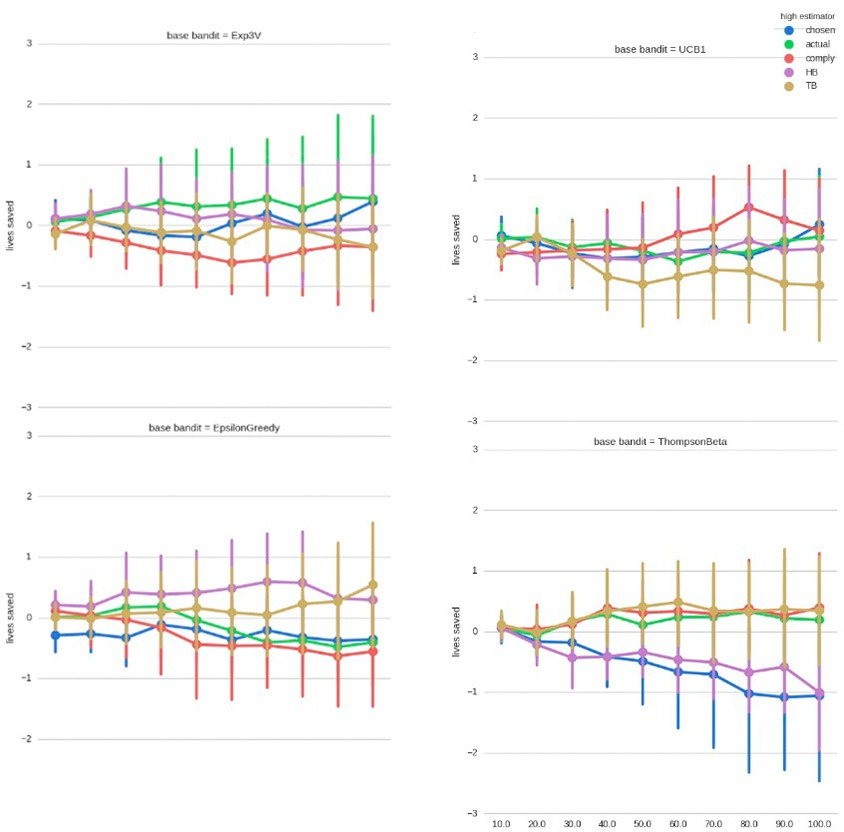
\includegraphics[width=1\columnwidth]{bandit/figs/fig1a.jpeg}
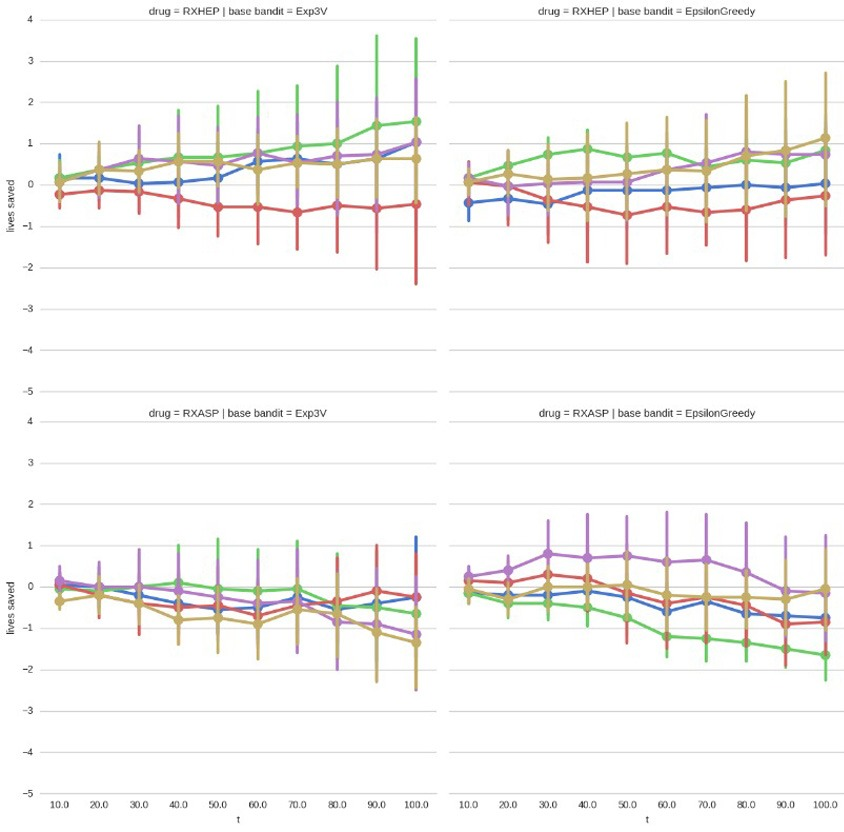
\includegraphics[width=1\columnwidth]{bandit/figs/fig1b.jpeg}
\caption{\textbf{14 Day survivals:} average lives saved over uniform random policy per 10,000 patients in simulated trials of Aspirin and Heparin.}
\label{fig1}
\end{center}
\end{figure} 

We simulated 10,000 patients per run, which allowed us to not oversample the data in any single simulation; 2000 runs were performed, all algorithms were tested against the same draw of the run to minimize unnecessary sampling variation. 

The \texttt{EXP3} gamma parameter was set ahead of time to 0.085, a choice determined by the regret-bounds for $T=10000$ and $K=2$ or $3$. Epsilon-Greedy used a standard annealing schedule. No data dependent parameter tuning was used.
The simulation was carried out by creating a ``counter-factual patient'' by sampling (i.i.d.) one patient from each of the treatment and control groups in the clinical trial. If the algorithm selected the treatment, it then receives the reward and observes the action taken by the subject sampled form the treatment group, and vice versa for the control.


Empirically, \texttt{TB} achieved a surplus of 8.9 extra survivals (that is, human lives) with 95\% confidence interval $[8.1,9.7]$, relative to the randomized baseline.
\texttt{HB} with \texttt{Epsilon Greedy} as the base algorithm achieved a surplus of 9.2 (CI: $[8.3,10.0]$)
In contrast, the best performing strategy that was not compliance aware was Thompson sampling, which yielded 7.9 extra survivals (CI: $[7.2,8.7]$). 

The gains were largely concentrated in the Aspirin trial, which is consistent with the lack of benefits or severe ill effects found in the original study \cite{ist:97} for heparin, and with the small but beneficial effect found for aspirin. 
If the underlying treatment has no positive or negative effect, side-information after the fact alone cannot be helpful.
Note that \actual, and to a lesser extent \comply, performed better than either \chosen\, or the hybrid algorithms. However, these are problematic be used directly since no guarantees apply, their worst case performance unbounc. The performance of the hybrids benefits from the information encoded in \actual\, and \comply\, whilst keeping the guarantees of \chosen. 


A striking secondary finding is the strong interaction between the learning algorithm and the nature of the feedback used. In particular our naive implementation of \texttt{EXP3} performed extremely badly under both \actual\, and \comply, in both the aspirin and heparin simulations. As a result, it is remarkable is that \texttt{EXP3} performs well when used as a top-level algorithm in \texttt{HB} in both trials, and other algorithms on the same data with the same protocol are able to learn better than chosen, while \texttt{EXP3} does worse than random (note the \texttt{EXP3} guarantees are only for the \chosen\, protocol, so do not apply here).



\section{Synthetic Data}


To better understand the behavior of the algorithms in a more varied range of settings, we present results of simulations with synthetic data.
The first simulation illustrates example~2. For comparison, $T$ is kept at 10,000, and we simulated the binary outcome case. We assigned half the patients to rich and half to poor randomly. Rich patients always take the treatment and their outcome, which would otherwise be 1 with $p=1$, becomes 1 with  $p=0.75$. Poor patients only take the treatment when prescribed, their favorable outcome has probability $p=0.5$ without treatment; taking the treatment reduces the probability of a favourable outcome to $p=0.25$. Fig.~2 shows that the performance of \actual\, and \comply\, is much worse than \chosen\, and the hybrid algorithms.



\subsection{Selection of treatment on correlated unobservables}

Consider a harmful treatment. Suppose there are two sub-populations with equal numbers of each. The first consists of rich, healthy patients who always take the treatment. The second consists of poor, less healthy patients who only take the treatment if prescribed. Finally, suppose the treatment reduces survival by 0.25. Assume that the right patients, if they didn't take the treatment would all do well (receive reward of 1), but they all take it, so face only a 0.75 chance of survival. Poor patients who face a baseline survival of 0.75, only take the treatment if instructed, which brings them down from 0.5. Results are for 100 samples.

%\begin{tabular}{llrrrrrlrrrrrl}
\toprule
   &               &   surplus &         &        &        &             &                        &     t &        &       &        &              &                   \\
   &               &      mean &  median &   amin &   amax &         std &                     ci &  mean & median &  amin &   amax &          std &                ci \\
\midrule
HB & EpsilonGreedy &           &         &        &        &             &                        &       &        &       &        &              &                   \\
   & Exp3V &  174.1895 &  153.00 & -263.5 &  533.5 &  147.946788 &    (165.219, 183.2735) &  5500 &   5500 &  1000 &  10000 &  2873.718542 &  (5329.0, 5679.0) \\
   & ThompsonBeta &  142.0385 &  119.75 & -474.0 &  524.0 &  155.149882 &    (132.3765, 151.801) &  5500 &   5500 &  1000 &  10000 &  2873.718542 &  (5324.0, 5678.0) \\
   & UCB1 &  185.5045 &  169.75 & -380.5 &  634.5 &  169.553899 &    (174.9045, 195.937) &  5500 &   5500 &  1000 &  10000 &  2873.718542 &  (5320.0, 5679.0) \\
TB & EpsilonGreedy &  164.1275 &  137.75 &  -92.5 &  526.5 &  126.324350 &   (156.5355, 172.1095) &  5500 &   5500 &  1000 &  10000 &  2873.718542 &  (5323.0, 5675.0) \\
   & Exp3V &  289.3035 &  298.50 & -668.0 &  680.5 &  214.914664 &    (275.9625, 302.343) &  5500 &   5500 &  1000 &  10000 &  2873.718542 &  (5321.0, 5680.0) \\
   & ThompsonBeta &  297.4625 &  303.75 & -678.5 &  698.5 &  207.917822 &   (284.0285, 310.1175) &  5500 &   5500 &  1000 &  10000 &  2873.718542 &  (5325.0, 5677.0) \\
   & UCB1 &  306.1865 &  312.00 & -631.0 &  699.5 &  202.821630 &   (293.4995, 318.3395) &  5500 &   5500 &  1000 &  10000 &  2873.718542 &  (5321.0, 5678.0) \\
actual & EpsilonGreedy &  312.8985 &  312.50 & -602.0 &  676.5 &  197.493261 &     (300.614, 325.125) &  5500 &   5500 &  1000 &  10000 &  2873.718542 &  (5317.0, 5672.0) \\
   & Exp3V & -267.7995 & -260.00 & -614.5 &    0.0 &  153.773319 &    (-277.54, -258.495) &  5500 &   5500 &  1000 &  10000 &  2873.718542 &  (5318.0, 5678.0) \\
   & ThompsonBeta & -315.3935 & -311.25 & -675.5 &  -19.5 &  180.209696 &  (-326.0585, -303.666) &  5500 &   5500 &  1000 &  10000 &  2873.718542 &  (5321.0, 5672.0) \\
   & UCB1 & -228.9745 & -213.75 & -642.0 &   13.0 &  141.402885 &  (-237.771, -220.2625) &  5500 &   5500 &  1000 &  10000 &  2873.718542 &  (5318.0, 5674.0) \\
chosen & EpsilonGreedy &  -79.1915 &  -66.75 & -308.0 &   54.5 &   71.682714 &      (-83.738, -74.79) &  5500 &   5500 &  1000 &  10000 &  2873.718542 &  (5321.0, 5672.0) \\
   & Exp3V &  294.8915 &  292.25 &  -38.5 &  616.5 &  161.242274 &    (284.8325, 304.806) &  5500 &   5500 &  1000 &  10000 &  2873.718542 &  (5320.0, 5681.0) \\
   & ThompsonBeta &  249.8975 &  238.75 & -151.0 &  615.5 &  169.257902 &    (239.5855, 260.232) &  5500 &   5500 &  1000 &  10000 &  2873.718542 &  (5325.0, 5681.0) \\
   & UCB1 &  328.8535 &  327.25 & -118.5 &  687.5 &  181.694511 &   (317.5725, 340.0625) &  5500 &   5500 &  1000 &  10000 &  2873.718542 &  (5322.0, 5681.0) \\
comply & EpsilonGreedy &  284.2595 &  278.75 &   19.5 &  625.5 &  166.451764 &   (273.7875, 294.4835) &  5500 &   5500 &  1000 &  10000 &  2873.718542 &  (5326.0, 5671.0) \\
   & Exp3V &  -48.2795 &  -70.00 & -600.5 &  574.0 &  292.451920 &     (-66.124, -29.997) &  5500 &   5500 &  1000 &  10000 &  2873.718542 &  (5320.0, 5682.0) \\
   & ThompsonBeta & -290.8165 & -281.00 & -643.5 &  262.5 &  182.486686 &   (-302.0395, -279.63) &  5500 &   5500 &  1000 &  10000 &  2873.718542 &  (5318.0, 5672.0) \\
   & UCB1 &   -6.7395 &   -7.50 & -672.5 &  590.5 &  228.589111 &       (-20.708, 7.563) &  5500 &   5500 &  1000 &  10000 &  2873.718542 &  (5320.0, 5672.0) \\
\bottomrule
\end{tabular}


%\begin{tabular}{llrrrrrlrrrrrl}
\toprule
   &               &   surplus &         &        &        &             &                        &     t &        &       &        &              &                   \\
   &               &      mean &  median &   amin &   amax &         std &                     ci &  mean & median &  amin &   amax &          std &                ci \\
\midrule
HB & EpsilonGreedy &           &         &        &        &             &                        &       &        &       &        &              &                   \\
   & Exp3V &  174.1895 &  153.00 & -263.5 &  533.5 &  147.946788 &    (165.219, 183.2735) &  5500 &   5500 &  1000 &  10000 &  2873.718542 &  (5329.0, 5679.0) \\
   & ThompsonBeta &  142.0385 &  119.75 & -474.0 &  524.0 &  155.149882 &    (132.3765, 151.801) &  5500 &   5500 &  1000 &  10000 &  2873.718542 &  (5324.0, 5678.0) \\
   & UCB1 &  185.5045 &  169.75 & -380.5 &  634.5 &  169.553899 &    (174.9045, 195.937) &  5500 &   5500 &  1000 &  10000 &  2873.718542 &  (5320.0, 5679.0) \\
TB & EpsilonGreedy &  164.1275 &  137.75 &  -92.5 &  526.5 &  126.324350 &   (156.5355, 172.1095) &  5500 &   5500 &  1000 &  10000 &  2873.718542 &  (5323.0, 5675.0) \\
   & Exp3V &  289.3035 &  298.50 & -668.0 &  680.5 &  214.914664 &    (275.9625, 302.343) &  5500 &   5500 &  1000 &  10000 &  2873.718542 &  (5321.0, 5680.0) \\
   & ThompsonBeta &  297.4625 &  303.75 & -678.5 &  698.5 &  207.917822 &   (284.0285, 310.1175) &  5500 &   5500 &  1000 &  10000 &  2873.718542 &  (5325.0, 5677.0) \\
   & UCB1 &  306.1865 &  312.00 & -631.0 &  699.5 &  202.821630 &   (293.4995, 318.3395) &  5500 &   5500 &  1000 &  10000 &  2873.718542 &  (5321.0, 5678.0) \\
actual & EpsilonGreedy &  312.8985 &  312.50 & -602.0 &  676.5 &  197.493261 &     (300.614, 325.125) &  5500 &   5500 &  1000 &  10000 &  2873.718542 &  (5317.0, 5672.0) \\
   & Exp3V & -267.7995 & -260.00 & -614.5 &    0.0 &  153.773319 &    (-277.54, -258.495) &  5500 &   5500 &  1000 &  10000 &  2873.718542 &  (5318.0, 5678.0) \\
   & ThompsonBeta & -315.3935 & -311.25 & -675.5 &  -19.5 &  180.209696 &  (-326.0585, -303.666) &  5500 &   5500 &  1000 &  10000 &  2873.718542 &  (5321.0, 5672.0) \\
   & UCB1 & -228.9745 & -213.75 & -642.0 &   13.0 &  141.402885 &  (-237.771, -220.2625) &  5500 &   5500 &  1000 &  10000 &  2873.718542 &  (5318.0, 5674.0) \\
chosen & EpsilonGreedy &  -79.1915 &  -66.75 & -308.0 &   54.5 &   71.682714 &      (-83.738, -74.79) &  5500 &   5500 &  1000 &  10000 &  2873.718542 &  (5321.0, 5672.0) \\
   & Exp3V &  294.8915 &  292.25 &  -38.5 &  616.5 &  161.242274 &    (284.8325, 304.806) &  5500 &   5500 &  1000 &  10000 &  2873.718542 &  (5320.0, 5681.0) \\
   & ThompsonBeta &  249.8975 &  238.75 & -151.0 &  615.5 &  169.257902 &    (239.5855, 260.232) &  5500 &   5500 &  1000 &  10000 &  2873.718542 &  (5325.0, 5681.0) \\
   & UCB1 &  328.8535 &  327.25 & -118.5 &  687.5 &  181.694511 &   (317.5725, 340.0625) &  5500 &   5500 &  1000 &  10000 &  2873.718542 &  (5322.0, 5681.0) \\
comply & EpsilonGreedy &  284.2595 &  278.75 &   19.5 &  625.5 &  166.451764 &   (273.7875, 294.4835) &  5500 &   5500 &  1000 &  10000 &  2873.718542 &  (5326.0, 5671.0) \\
   & Exp3V &  -48.2795 &  -70.00 & -600.5 &  574.0 &  292.451920 &     (-66.124, -29.997) &  5500 &   5500 &  1000 &  10000 &  2873.718542 &  (5320.0, 5682.0) \\
   & ThompsonBeta & -290.8165 & -281.00 & -643.5 &  262.5 &  182.486686 &   (-302.0395, -279.63) &  5500 &   5500 &  1000 &  10000 &  2873.718542 &  (5318.0, 5672.0) \\
   & UCB1 &   -6.7395 &   -7.50 & -672.5 &  590.5 &  228.589111 &       (-20.708, 7.563) &  5500 &   5500 &  1000 &  10000 &  2873.718542 &  (5320.0, 5672.0) \\
\bottomrule
\end{tabular}



\begin{figure}
	\centering	
	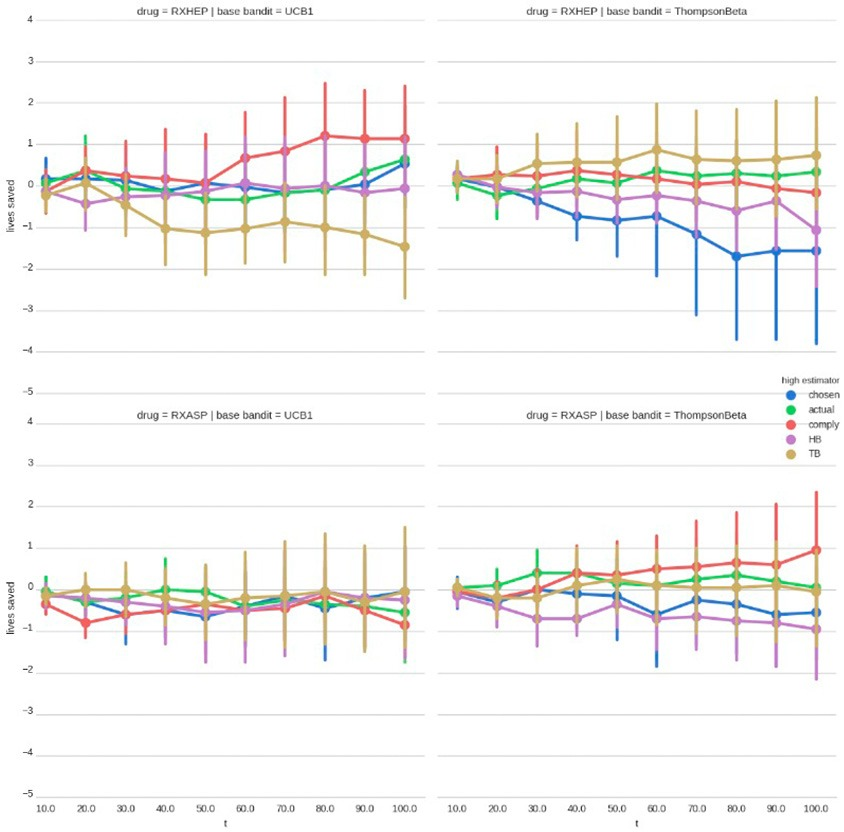
\includegraphics[width=1\columnwidth]{bandit/figs/ex2.jpeg}\hspace{1cm}
	\label{fig:ex2}
	\caption{Worse than random regret across estimators with naive uses of compliance awareness with simulated data from 100 patients sampled from a model of a harmful treatment that is profound by selection into treatment.}
\end{figure}



\subsection{Small T}

The second simulation concerns small $T$. A motivation for very small $T$ adaptive clinical trials is provided by rare diseases. The overall size of the patient population is by construction severely restricted in this setting.  The priors for the mechanisms of action are also often poorly understood, so potential alternative treatments can have radically different probabilities of success. We simulate a $T=12$ adaptive trial with binary outcomes, with two treatments and expected rewards drawn uniformly from the unit interval, and compliance uniformly at random. We sample 1,000 such simulations.
While our bounds are vacuous in this settings, it is interesting that there is on average an  improvement from taking the noncompliance information into account.


\begin{figure}[t]
	\centering	
	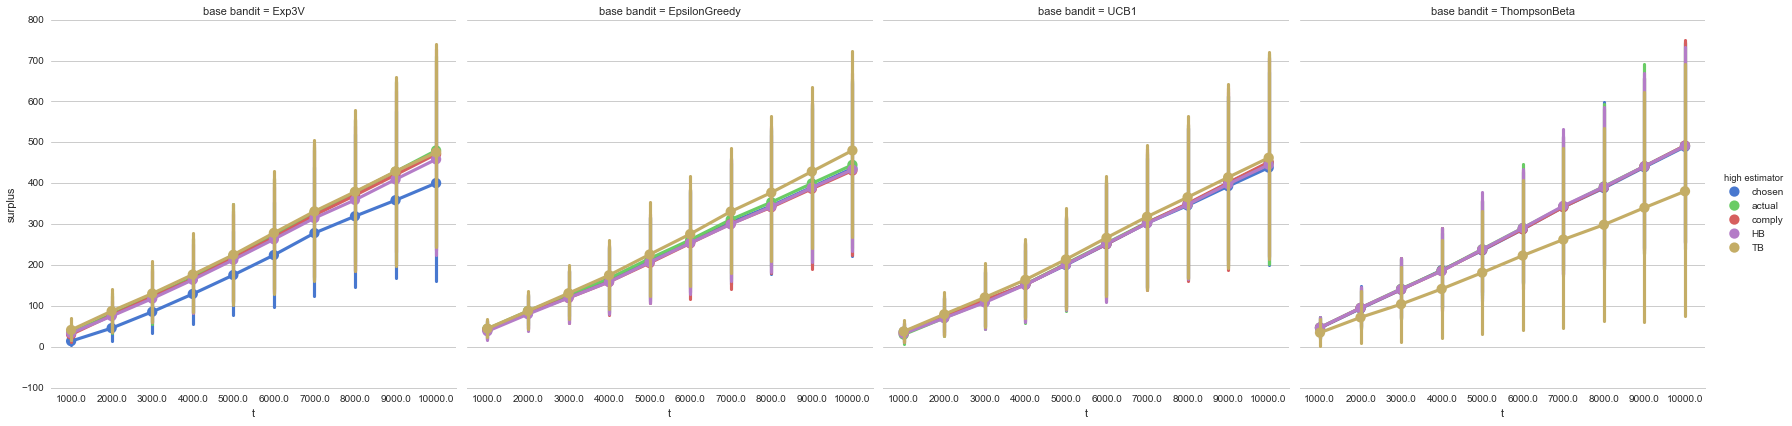
\includegraphics[width=1.5\columnwidth, angle=90]{bandit/figs/ex3.png}\hspace{1cm}
	\label{fig:ex3}
	\caption{12 patients, a not uncommon size of clinical trials in rare diseases or neonatal populations.}
\end{figure}





\subsection{Noncompliance for Best Arm}


A natural scenario for noncompliance and one that offers substantial potential is when the subject is better informed than the algorithm, and realizes they know a better alternative. 
This provides potentially huge practical advantages, specially in situations with very large numbers of a priori low expectation but high variance actions. 
They allow later subjects to benefit from the information that previous subjects bring to the mechanism, while current compliance unaware algorithms not only waste this information but hurt later subjects as it unnecessary raises the apparent variance of the rewards in the arms (since the chosen arm may indeed be very bad relative to the actual arm).




\begin{figure}[t]
	\centering	
	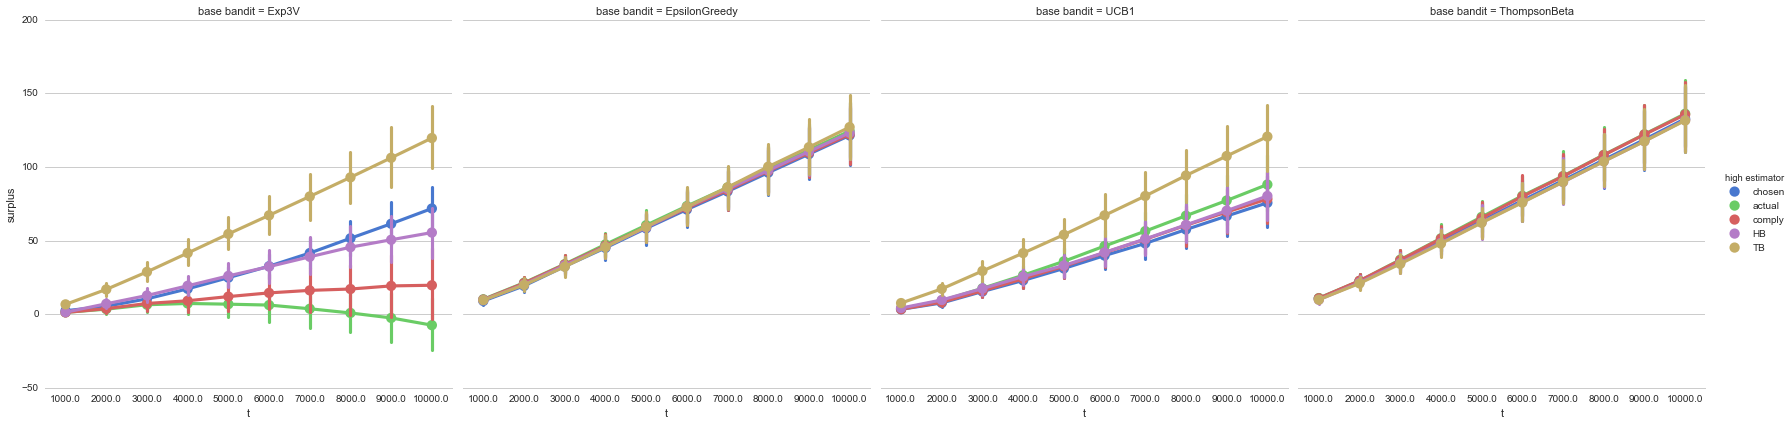
\includegraphics[width=1.5\textwidth, angle=90]{bandit/figs/ex4.png}\hspace{1cm}
	\label{fig:ex4}
	\caption{Noncompliance for best arm}
\end{figure}



%     def __init__(self,foo ):
%         n_arms=2
%         self.arm_value = 0.5+0.25*np.random.random(n_arms)
%         self.n_arms = n_arms
%     def draw_subject(self):
%         prefered_arm = stochastic_argmax(self.arm_value)
%         prefered_reward = random.binomial(1,self.arm_value[prefered_arm])
%         r = []
%         for i in range(self.n_arms):
%             if self.arm_value[i] / self.arm_value[prefered_arm] < random.random(): #informative noncompliance
%                 r.append((prefered_arm,prefered_reward))
%             else:  #compliers 
%                 r.append((i,  random.binomial(1,self.arm_value[i])))
%         return r

% example3= sim( nsim=100, T=10001, DGP=NoncomplianceForBestArm , drug="Better arm")
% display_results(example3.loc[example3['t'] == 10000].drop('t',1))



%\subsection{Independent Noncompliance and Rewards}

%We now simulate a neutral model, where compliance is unrelated to the rewards of the arm.
% #always or never takers. current simulation model is not rich enough for defiers, todo?
% class IndependentNoncomplianceAndRewards():
%     def __init__(self,foo):
%         n_arms=2
%         self.arm_value = 0.9+0.1*np.random.random(int(n_arms))
%         # todo add effect_magnitude=1
%         self.n_arms = n_arms
%     def draw_subject(self):
%         if random.random()<0.9: #compliers 
%             r=[(i, random.binomial(1,self.arm_value[i])) for i in range(self.n_arms)]
%         else:   #always takers
%             actual = categorical_draw(self.arm_value)
%             reward = random.binomial(1,self.arm_value[actual])
%             r= [(actual, reward) for i in range(self.n_arms)]
%         return r

    
% example4= sim( nsim=100, T=10001, DGP=IndependentNoncomplianceAndRewards , drug="example")
% display_results(example4.loc[example4['t'] == 10000].drop('t',1))







%think of the babies http://www.ncbi.nlm.nih.gov/pmc/articles/PMC2778326/



%We have two simulations, one in which noncompliance is independent of everything, and one where noncompliance is towards the higher expectation treatment.

%This is a boring figure, not rue what to say about it.
%%%%%%%%%%%%%%%%%%%%%%%%%%%%%%%%%%%%%%%%%%%%%%%%%%%%%%%%%%%%%%%%%%%%%%%%%%%%%%%%%%%%%%%%
%\subsection{Conclusions}

%Empirically, \texttt{TB} achieves a surplus of 8.9 extra survivals (that is, human lives) and \texttt{HB} achieves 9.2 surplus lives compared with 7.9 for the best classical algorithm. This suggests hybrid algorithms can make a significant difference to clinical outcomes.

% TODO, add note on composability and comparing to relatively well understood baselines. plug and play.




\part{Mechanism for Optimal Decision Elicitation from Many Experts}

\chapter{A Single Decision}
\label{cha:market}
%\epigraph{Give the people what they want\\ when they want it \\
%And they wants it all the time}{Parliament \\ Supergroovalisticprosifunkstication}

\section{Introduction}

%cahnnel from roth economist as enginerr
%Since then, economists have gained significant experience in practical market
%design. One thing we learned from this experience is that transactions and institutions %matter at a level of detail that economists have not often had to deal with,
%and, in this respect, all markets are different. But there are also general lessons.
%This essay will consider some ways in which markets succeed and fail by looking at
%some common patterns we see of market failures, and how they have been fixed."
%3. Make it safe to participate in the market as simply as possible, as opposed to
%transacting outside of the marketplace, or engaging in strategic behavior that reduces
%overall welfare.


This chapter considers a subject facing a decision, who wishes to incentivize multiple experts in providing advice so as to pick a decision that maximizes the rewards the subject receives, while maintaining the freedom of the subject.
Experts do not have intrinsic interest in the action the subject chooses or actually takes, nor do they face any costs in acquiring their signals.

Preserves subjects freedom is a inherently desirable practical design criterion as it enables no-regret exploration on the part of the subjects. Subject remains at all points in control of the decision, and so trying the mechanism cannot reduce their choices or their expected welfare.\footnote{One can set a reserve price of the advice auction to the expected value of the action the agent would have picked if they did not participate in the mechanism. As long as the reserve price is set apriori or alternative reports from the non-winning bidders are the only thing used to set it, the incentives do not change from those analyzed here.}.



The main contribution of this chapter is casting this setting as one of a single unit efficient allocation with interdependent valuations (\cite{milgrom1982theory,maskin1992auctions,ausubel1999generalized,mclean2004informational,roughgarden2016optimal,eden2018interdependent}).
This allows us to leverage existing results in that setting, which provide both necessary conditions for efficient allocations (single crossing conditions on the signal structure) and impossibility results when those are not met.

% Each bidder reports her type to the auctioneer. Given the reports, the auctioneer determines the allocation that maximizes surplus.
%The payment rule is the following extension of Vickrey auction pricing: a bidder is charged for a given unit that she wins according to valuations evaluated at the minimum signal that she could have reported and still won that unit.



The key conceptual contribution that allows this is to consider the allocation not over the decisions, but instead over the experts providing the advice. 
The item to be allocated is the right to observe the signal reports, provide the advice and a (linear) share of the reward obtained by the subject.
We term these mechanisms \emph{advice auctions}.
The term advice is chosen to highlight that the decision is not ultimately determined by the market, thus preserving the subject's freedom.
The term auction highlights that this procedure does not produce a sequence of prices through time.
It is this simultaneous nature that allows us to side-step the negative (from the perspective of freedom) results that constrain sequential mechanisms to having full support over actions in order to provide  incentives.

Sharing rewards after choosing what decision to advise is neither a pure private value (since the optimal choice conditional on information makes the value the same for everyone) nor pure common value (since the ability to select the optimal choice given access to the other signals might vary across agents).

A advantage of this setting to having a mechanism that directly outputs a chosen action is that it allows for the expert making the recommendation to have different influences on subject (i.e. some experts may be more persuasive).
If the mechanism output was a choice to advise the subject directly, we would have to restrict the expected reward the subject receives not to depend on which expert submitted which report. This can be seen as  a limit on subject freedom (since it it is an external constraint).
Further, by having the mechanism select the expert instead of the choice, the natural extension to the more practical mechanisms that do not require the mechanism to have access to the valuation functions, but instead rely on the highest bidder to be able to aggregate signals effectively.

%This closely follows work on efficiency allocation with interdependent values , and our mechanism has the same two steps: first agents submit their signals so as to be able to determine the probabilities over states of the world, and the results of that are used to pick an efficient allocation in what is private .  


\subsection{Limits to Subject Freedom in Sequential Proper Scoring Rule Based Decision Markets}

One way to incentivize them is by applying the machinery of prediction markets based on sequentially shared proper scoring rules to the expected reward conditional on the action.
A challenge that presents itself is how to settle the markets for the reward conditional on the action which is not taken.
One natural approach is to void the trades in the markets for these actions, this being the originally proposed mechanism in this line of work \cite{hanson2002decision}, and only settling the markets where actions are taken.
While seemingly natural, this is not incentive compatible for the experts, even in the weak myopic sense, as shown in \cite{othman2010decision}. 

To understand why this is the case, consider a last trader facing the prediction market (sequential proper scoring rule)  where the  price is correct (matches the expected reward) for the optimal action but there is some other action that is misprinted. The profit maximizing move for this trader is to lower the price of the optimal action below the true price of the previously misprinted action, and correct the mispriced action to its true  price. 
The utility maximizing subject would then carry out the suboptimal action, the expert would be rewarded for correctly predicting it and would receive no punishment for the error they introduced into the reward of the optimal action. 
%A mechanism is called Bayes Nash Incentive Compatible (BNIC) if there is a equilibrium were every agent reports their signal truthfully and this maximizes their reward in expectation (over the state of the world).
The mechanism proposed in \cite{hanson2002decision} is not BNIC for the experts who provide advice, as witnessed by the example above (and shown in \cite{othman2010decision,chen2014eliciting}).
More generally, any sequential proper scoring rule based mechanism that is incentive compatible for the experts is incompatible with maintaining the subject's freedom to select the action that appears optimal ex-post (\cite{ chen2014eliciting}). 

%Interdependent Values without Single-Crossing
%Alon Eden, Michal Feldman, Amos Fiat, Kira Goldner
%We consider a setting where an auctioneer sells a single item to n potential agents with {\em interdependent values}. That is, each agent has her own private signal, and the valuation of each agent is a known function of all n private signals. This captures settings such as valuations for artwork, oil drilling rights, broadcast rights, and many more. 


%In the interdependent value setting, all previous work has assumed a so-called {\sl single-crossing condition}. Single-crossing means that the impact of agent i's private signal, si, on her own valuation is greater than the impact of si on the valuation of any other agent. It is known that without the single-crossing condition an efficient outcome cannot be obtained. We study welfare maximization for interdependent valuations through the lens of approximation. 


%\cite{eden2018interdependent}
%We show that, in general, without the single-crossing condition, one cannot hope to approximate the optimal social welfare any better than the approximation given by assigning the item to a random bidder. 
%Consequently, we introduce a relaxed version of single-crossing, {\sl c-single-crossing}, parameterized by c≥1, which means that the impact of si on the valuation of agent i is at least 1/c times the impact of si on the valuation of any other agent (c=1 is single-crossing). Using this parameterized notion, we obtain a host of positive results. 


% The first step of our procedure maps to the setting of 
% https://www.sas.upenn.edu/~apostlew/paper/pdf/auctionrevised.pdf
%and more generally
% TE2015 



\subsection{Summary and Outline}

%TODO: garrett says more clear explanation. make explicit pointer to background section, and make paragraph of sentence.
%The core of the problem which emerges upon using the machinery of prediction markets in the decision setting is that

The rest of the chapter is structured as follows.
We first introduce a formal model and notation.
We then present advice auctions as a direct mechanism, show when they are truthful, as well as their limits.
We then consider two practical indirect variations of the procedure, which removes the need for the mechanism to have any knowledge of valuations, and consider sufficient conditions for their efficiency and truthfulness.  



\section{Model}



As before, the subject seeks advice on a decision they will take from some finite set of alternatives $A$, let $c$ be the choice that is given as advice to the subject and $a$ the decision that the subject actually takes.
The rest of our model and notation largely follow that of \cite{eden2018interdependent}.%\footnote{Relative to their notation and to maintain coherency with the other chapters in the thesis, in our setting the number of potential actions is $q$ instead of $k$, while  }.
Each expert $i \in \{1, \ldots, n\}$ receives a single signal $s_i$ which is known only to expert $i$.
Potential signals for bidder $1 \leq i\leq n$ form a discrete signal space $S_i$.
Let $\vec{s}=(s_1,s_2,\ldots,s_n)$ be a signal profile.
The reward $r$ that the subject receives depends on their chosen action $a$ and the underlying state of the world as determined by the signal profile $\vec{s}$.
Let $\vec{s}_{-i}$ denote all signals but $s_i$, and let $(s_i',\vec{s}_{-i})$ denote the profile $\vec{s}$ where $s_i$ has been replaced with $s'_i$. 
Since $r$ does not depend on the choice of $c$ by the expert, and that at the point the mechanism is run $a$ has not been selected, we use the following reduced form  value function for the value of the rights bundle to expert $i$: $v_i: \times_i S_i \rightarrow \mathbb{R}_{\geq 0}$, which maps every signal profile to the expected value of linear share of the reward  $\alpha r$.


Each expert reports a signal $b_i$, and the vector of reported signals is $\vec{b}=( b_1, b_2, \ldots, b_n)$.
Each possible signal profile $\vec{s}$ corresponds to an underlying state of the world, this includes both inherent physical properties of the subject and the actions, as well as the subjects probability of choice of $a$ in response to different choices of $c$.
%Without loss of generality, assume $S_i=\{0,1,\ldots,q_i\}$.


%This value is given by $\alpha r(\vec{s})$
The valuation functions for all bidders $i$ are monotone non-decreasing in every signal $s_j$ for all $j$.%\footnote{Both of these assumptions are without loss of generality; the space of potential signals can alwyas be , while the ordering of the signals is arbitrary, so they can always be sorted into monotone non-decreasing.}

Mechanisms are a pair $(x,p)$, where $x$ is a set of allocation functions $x=\{x_1(\vec{b}),\ldots,x_n(\vec{b})\}$ satisfying $\sum_i x_i(\vec{s}) \leq 1$ for all possible $\vec{b}$, and $p$ a set of payment functions  $p=\{p_1(\vec{b}),\ldots,p_n(\vec{b})\}$.
An allocation function $x_i:\times_j S_j\rightarrow [0,1]$ maps every bid profile $\vec{b}$ to the probability that expert $i$ gets allocated.
A payment rule $p_i: \times _j S_j \rightarrow \cR$ maps the reported signals $\vec{b}$ to the expected payment from bidder $i$. Experts are risk neutral, so their expected utility is quasilinear, given in the reduced form by $x_i (\vec{b}) \cdot v_i(\vec{s}) - p_i(\vec{b})$ where $\vec{s}$ is the true signal profile of the experts.


%One cannot hope for truth-telling to be a dominant strategy for the experts. One expert's misreport can cause other experts to also misreport to compensate. Thus the strongest incentive-compatibility (IC) notion that we can hope for is in this setting is truthfulness is an ex-post Nash Equilibrium. That is it is in every agent $i$'s best interest to report his true signal $s_i$ given that all other agents reported the true signal profile $\vec{s}_{-i}$:
$$x_i(\vec{s}) \cdot v_i(\vec{s}) - p_i(\vec{s}) \geq x_i(b_i, \vec{s}_{-i}) \cdot v_i(\vec{s}) - p_i(b_i, \vec{s}_{-i})  \quad \quad \quad  \forall \vec{s} \in \times _{j} S_j, b_i \in S_i. \quad\quad\quad [\text{IC}]$$




%As in \cite{mclean2004informational} an experts  information may be of two qualitatively different kinds: information about the objective characteristics of the subject and the effects of their alternative decisions and how generally persuasive they are to find the recommended action.
%Idiosyncratic information about the agent himself: their ability to aggregate the signals efficiently, and how persuasive the would result as the advisors who selected $c$ in the second stage of the game. 
%The former is of interest to other agents—and consequently is the cause of the interdependence of agents’ values—while the latter is irrelevant to other agents in calculating their values.


\section{A Direct Reward Sharing Mechanism}

The simplest class of mechanisms to incentivize advice is based on sharing a fraction of the rewards with the experts. For the single expert case this is mentioned by \cite{othman2010decision}. Here the idea is extended to the multiple experts case. We do this by instantiating our notion of advice auctions with a simple mechanism,
the generalized VCG mechanism proposed by \cite{maskin1992auctions}. This mechanism is \emph{direct} in the standard sense that agents report their signals. 

The core of the mechanism is simple. Since there is knowledge by the mechanism over the value function for a given vector of signals, it can use the reported signals to select the highest value expert. The net payment to that expert is then just his share of the reward minus his value at the lowest signal he could have misreported and still obtained the allocation give the other reports. More formally:

\begin{mech}\label{mech:Direct}[Direct Reward Share VCG]
Then mechanism gives the rights bundle to the expert $i^*$ with the highest valuation under the reported signals. That is, the allocation rule is:

$$x(\vec{s}) = i \quad \quad\quad \text{when} \quad\quad\quad x_j(\vec{s}) = \begin{cases} 1 & \text{if } j=i \\ 0 & \text{otherwise.} \end{cases}$$

This lets the expert $i^*$ observe  $\vec{b}$ and then select $c$.
Then subject observes $c$ and $\vec{b}$, takes their action $a$ and receives reward $r$, which the mechanism observes. 

The non selected experts receive no payment, while the selected expert $i^*$ receives their share $\alpha$ of the reward $r$ minus the value of the share of the reward at the lowest $b_i'$ (the critical signal) that would have still resulted in expert $i$ being selected. 
More formally, given signals for agents $\neq i$, $\vec{s}_{-i}$, the {\sl critical signal} for $i$ is: if there exists some $b_i$ such that $x_i(s_{-i},b_i)=1$ then set $b_i^*=\min_{b_i} x_i(s_{-i},b_i)=1$, otherwise there is no critical signal for $i$.
Thus, the payment rule is:

$p_i= \alpha r - v_i(\vec{s}_{-i},b_i^*)$

\end{mech}

An allocation function $x_i$ is called {\sl deterministic} if $x_i(\vec{b})\in \{0,1\}$ for all $i$ and all $\vec{b}$.
The generalized direct VCG mechanism is deterministic and prior-free.

\subsection{Truthfulness with Single Crossing Signals}

\begin{defn}[Monotonicity]
	An allocation function $x_i$ is said to be monotone if for every $\vec{b}_{-i}$, $x_i(\vec{b}_{-i},b_i)$ is monotone non-decreasing in the signal $b_i$.
\end{defn}

Truthful mechanisms can be characterized as follows \cite{roughgarden2016optimal}.

\begin{prop}\label{prop:char-ic}
	Monotonicity is a necessary and sufficient condition for allocation functions $x$ to be \emph{implementable}, {\sl i.e.}, there exist payment functions $p$ such that the mechanism $(x,p)$ is truthful.  Moreover, an analogue of Myerson's payment identity holds, so the payment is uniquely determined by the allocation function.
\end{prop}

It follows that constructing a truthful mechanism is equivalent to constructing a monotone allocation function.
For deterministic truthful mechanisms, the payment identity of \citet{roughgarden2016optimal} implies the following about the cost charged to a chosen expert (from \cite{eden2018interdependent}).

\begin{prop}\label{prop:deterministic_payment}
	Let agent $i$ be the allocated winner at report profile $\vec{s}$ in a deterministic truthful mechanism. Then their cost is their value at the critical report.
\end{prop}


A single-crossing condition captures the idea that bidder $i$'s signal has a greater effect on experts $i$'s value than on any other experts's value. We follow the definition in \cite{eden2018interdependent}:

For $s_i = 1, \ldots, k_i$, define $\frac{\partial v_j(s_i, \vec{s}_{-i})}{\partial s_i} = v_j(s_i, \vec{s}_{-i}) - v_j(s_i - 1, \vec{s}_{-i})$.

\begin{defn}[Single-Crossing]
	A valuation profile is said to satisfy the single-crossing condition if for every expert $i$, for any set of other experts  signals $\vec{s}_{-i}$, and for every expert $j$, $$\frac{\partial v_i(s_i, \vec{s}_{-i})}{\partial s_i} \geq \frac{\partial v_j(s_i, \vec{s}_{-i})}{\partial s_i}.$$
\end{defn}


%We note that there also exists a weaker notion of single-crossing that only requires the inequality to hold at $\vec{s}$ for the bidder $i$ with the highest value, where $i \in \argmax_{k} v_k(\vec{s})$.

\begin{thm}
	There is a truthful and efficient ex-post Nash equilibrium of the DRSA mechanism when signals satisfy the single crossing property.
\end{thm}

\begin{proof}
Allocating to the bidder with the highest value is a monotone allocation rule, and therefore, according to Proposition~\ref{prop:char-ic} it is implementable. The cost for the rights bundle of the chosen expert is then just their value at their critical signal, which is the corresponding payment.
\end{proof}

Further, one cannot do better than this as per Proposition~\ref{prop:char-ic}, monotonicity of the allocation rule is necessary for a efficient and truthful mechanism with interdepedent values. Hence, without single-crossing, it is impossible to have a truthful advice auction in general.

This procedure for a direct advice elicitation mechanism based on the advice auction procedure was here instantiated using \cite{maskin1992auctions}  as the underlying auction mechanism. But the procedure is generic. It could be, for example, instantiated instead with the randomized mechanism of \cite{eden2018interdependent}, and would obtain the approximation properties that algorithm provides in auctions in our advice setting.


\section{Practical mechanisms: Advice Auctions}

The assumptions used in \cite{roughgarden2016optimal} that are used for the above result are extremely minimal relative to the existing literature in most of decision markets and auctions with interdependent values.

However, the mechanism having access to the value functions seems highly impractical in most potential applications.
Given the practical settings that motivate this work, 
we do not assume access by the mechanism to a the valuation functions, and consider two practical alternatives.


\subsection{A Bid and Signal Reward Sharing Mechanism}

The first modification one can do to make the payment of the highest bidder depend on the bid of the second highest, this removes the dependency of the payments function on the 

The challenge this faces is that the signals reports being submitted would not matter, so any signal report is in equilibrium. To correct this and create strict incentives again, we can add a further payment received by all experts that is also a linear share of the reward. This makes the truthful signaling equilibrium potentially strict.


\begin{mech}\label{mech:Direct}[Allocation with Bids, Reward Share with Signals (ABRSS)]
	Experts report both a bid and a signal, we slightly abuse notation and use $vec(s)$ to denote the reported signals, note their only use is to be displayed to the expert allocated to make the choice..
	Then the mechanism gives the rights bundle to the expert $i^*$ with the highest bid:
	
	$$x(\vec{b}) = i \quad \quad\quad \text{when} \quad\quad\quad x_j(\vec{b}) = \begin{cases} 1 & \text{if } j=i \\ 0 & \text{otherwise.} \end{cases}$$
	
	This lets the expert $i^*$ observe reported signals $\vec{s}$ and select $c$.
	Then subject observes $c$ and $\vec{b}$ and $\vec{s}$, takes their action $a$ and receives reward $r$, which the mechanism observes. 
	
	The non selected experts receive  payment $\beta r$, while the selected expert $i^*$ receives their shares $(\alpha + \beta) r$ of the reward minus the second highest bid, $b_{i^*-1}$.

	Thus, the payment rule is:
	
	$p_i^*= (\alpha + \beta)r - ,b_{i^*-1})$ and $p_{j\neq i^*} = \beta r$
\end{mech}



For this allocation rule to reach efficient allocation achieved by the direct mechanism, a stronger assumption on signal structure is needed. If we only require single crossing then the identity of the highest valuation expert can depend on interaction of their signals and those of other agents. Without access to the value function the mechanism cannot in general hope to achieve this allocation.
Thus beyond single crossing, we also require that the highest valuation expert must be so for any possible set of signals other than their own. In this case the allocation of this mechanism is efficient, since it coincides with the direct mechanisms allocation.

%MORE FORMALY

\begin{defn}[Single Signal Max Value]
	A valuation profile is said to satisfy the single-signal max value condition if highest value expert $i^*$ knows he is the highest value when given their signal, and for any set of other experts  signals $\vec{s}_{-i}$, and for every expert $j$, $$v_i(s_i, \vec{s}_{-i}) \geq  v_j(s_i, \vec{s}_{-i})}$$
\end{defn}


Note this property is not as strong as it may at first seem. If there is an expert who has the trust of the subject, understands what they find persuasive, and is sufficiently competent at evaluating the reported signals of others, it may be best able to select $c$ to maximize $r$ no matter the state of the world. Being able to see other experts' signals may however substantially raise the reward and hence the value of the highest valued expert.  


\begin{thm}
	There is a truthful and efficient ex-post Nash equilibrium of the ABRSS mechanism when signals satisfy the single signal max value property.
\end{thm}

\begin{proof}
	The highest value bidder bids his worst possible value given the other bids or anything higher (knowing he will win and be charged according to the second highest price makes him indifferent between these when others are truthful).
	Allocating to the bidder with the highest value is a monotone allocation rule, and therefore, according to Proposition~\ref{prop:char-ic} it is implementable. The cost for the rights bundle of the chosen expert is then the second highest bid, which is the corresponding payment.
\end{proof}



For contrast consider the identical mechanism but without the experts submitting their signals and receiving share $\beta$. 
 
\begin{mech}\label{mech:BidOnly}[Bid Only Advice Auction]
 	Each expert observes their signal and then report only a bid $b_i$. The mechanism gives the rights bundle to the expert $i^*$ with the highest bid:
 	
 	$$x(\vec{b}) = i \quad \quad\quad \text{when} \quad\quad\quad x_j(\vec{b}) = \begin{cases} 1 & \text{if } j=i \\ 0 & \text{otherwise.} \end{cases}$$
 	
 	This lets the expert $i^*$ observe reported bids $\vec{b}$ and then select $c$.
 	Then the subject observes $c$ and $\vec{b}$, takes their action $a$ and receives reward $r$, which the mechanism observes. 
 	
 	The non-selected experts receive  payment $\beta r$, while the selected expert $i^*$ receives their shares $(\alpha + \beta) r$ of the reward minus the second highest bid, $b_{i^*-1}$.
 	
 	Thus, the payment rule is:
 	
 	$p_i^*= (\alpha + \beta)r - ,b_{i^*-1})$ and $p_{j\neq i^*} = \beta r$
 \end{mech}
 
 For some very limited information structures the bidding mechanism still aggregates information efficiently. 
 For example, if each expert knows the expected outcome conditional on one action don't know what happens under other actions, and there is at least one expert who is informed about each action. These information structures correspond to the standard private values settings in the original VCG mechanism \cite{vickrey1961}.
 
 This kind of indirect mechanism is inherently limited when the value from the signals of experts are interrelated (as we proved before). Their bid cannot encode the full information contained in the signals, and thus this limits any mechanism that relies solely on single rounds of bids to aggregate information.
 
 To illustrate this, consider a setting that satisfies the single max bidder assumption. Denote by $i^*$ the experts whose valuation is higher than all other experts in every state of the world and who knows the subject trust them completely so if he wins $c=a$. Have a second expert whose value is $0$ in all states of the world\footnote{For example the expert might know the subject is biased and refuses to hear the expert due to color of their skin.} but has a binary independent signal $s_treat$ that determines which choice is best for the subject, without knowing $s_treat$ the two best choices have equal expected reward $r_uniform$, while knowing the value of the signal allows to select the appropriate choice and results in double the reward $2r_uniform$.
 Since his value is always 0 and so is his bid in equilibrium. 
 There is no prior-free way for the unpersuasive expert to encode his signal into their bid (even though they are incentivized to reveal their signal to get a higher $\beta$ payment). 
 Notice that there is no limit in the size of the gap in the rewards between the two allocations in general, as in the example above we can replace $2$ by any number.
 
 

\section{Conclusion}

This chapter shows how to use the bundle of rights perspective on advisers to recast the incentivizes for decision elicitation from multiple experts into the thriving literature on VCG with interdependent valuations.
We then use Proposition 1 of \cite{roughgarden2016optimal} to show that using the generalized VCG mechanism of \cite{maskin1992auctions} to allocate the rights results in a direct incentive compatible and efficient mechanism when signals have a single crossing property.
We then explore two practical variations of the mechanism that relax the assumption that the mechanism can access the value functions and that signals can be transmitted between experts.
We introduce a notion that shows when mechanisms that 


\chapter{A Sequence of Subjects}
%We consider a natural setting that generalizes both previous models.
%!TEX root = main.tex


\subsection{Introduction}

This chapter differs from the previous ones in it's relationship to the thesis. 
While previous we seek to extend the understanding of previously presented settings ( bandit algorithms and decision markets), this chapter seeks to introduce a new setting that contains these two.

The study of decision markets so far, including the previous chapter, have focused on a setting with a single decision and multiple advisers (\cite{hanson2002decision,othman2010decision,chen2014eliciting}).
This chapter poses a novel and natural extension of this setting motivated by the bandit setting: a sequence of subjects (patients in the medical motivation) as in that setting, and a fixed set of advisers (doctors) with access to side information about different patients expected values under different courses of action. 

We present a simple mechanism that preserves subjects freedom, argue that this is a inherently desirable practical design criterion as it enables no-regret exploration (since the subject remains at all point in control of the decision, and so trying the mechanism cannot reduce their choices).


Our motivating applications in medicine are suggestive of a sequence of similar decisions faced by a sequence of agents in order, all of whom face an individual choice on their own course of action.
Every day new patients perceive their symptoms, and they seek diagnoses and treatments. 
A corporation faces new investment opportunities with regularity, and similar opportunities appear to many firms that might not be competitive (for example vertical divisions in a conglomerate might be offered similar projects to automate part of their workflows and must choose to attempt them or not.
Scenarios such as these that motivate optimal decision elicitation are more naturally cast not as one-shot interactions, but as repeated games with many experts and a sequence of subjects who seek advice before making a decision which only affects them.
This combines the central aspects of bandits with compliance awareness (a sequence of choices and learning from past experience, where the actions of subjects are not bound to follow the algorithm choice) as well as elicitation of information from experts to enable optimal decisions without the advice being binding. 
Bounded regret algorithms with compliance awareness can be seen as addressing the special case where the experts' signals are known a priori to be uninformative, and thus only the experience can be learned from.

Our one-subject mechanism is the special case for $T={1}$, thus there is no role for exploration or learning from experience, since there are no future decisions to help inform.
A situation where experts always report their signals truthfully and have no knowledge over how to aggregate them beyond that possessed by the mechanism is equivalent to a compliance-aware contextual bandit problem. 
When contexts are constant across all time steps, the situation further reduces to a bandit problem with compliance awareness.
When the subject always follows the mechanism or $a$ cannot be observed, it reduces further  to the standard multi-armed bandit problem. 


Given the focus of this thesis on algorithms and mechanisms that preserve freedom, we do not wish to use forced randomization of the action taken which would allow for an unbiased estimator to be constructed and then used to set rewards. 
We can instead 

 
%A Bayes Nash analysis, looking at the set of equilibria and comparing the worst case rewards with it to the efficient outcome, is unappealing. 
%Not only does it require imposing strong assumptions on the information structures, but also it is not clear at all that markets of this complexity will be in equilibrium.
%A compelling argument in favor of such analysis is that no-regret dynamics push to the Nash Bayes set, (cite?) 


In contrast to the previous chapter's motivation in the literature, in this chapter our focus is on constructing a practical mechanism. 
The motivation for this switch is that the setting is natural, and no mechanisms (or the setting itself) have been previously proposed to the best of our knowledge.
In the two special cases of compliance aware bandits and single subject decision markets, the proposed mechanism reduces to the previously proposed mechanism.
There are, however, (infinite) other mechanisms that share this property. 

A key limitation of the one shot case is the need to randomize the agents choice to evaluate the counterfactual, and when there is a single agent these exploration (of the sub-optimal relative to the information reported) steps are not ex-post (signal reports) incentive compatible.
This is a different way to frame the result from the previous chapter on paying agents that bring uninformative signals: since evaluating the counterfactual value of the signal is not possible while preserving freedom of the agent taking the choice. 
In the terminology that motivates this thesis, they are not implementable while preserving the agents freedom.  
The most conceptually interesting change when moving to a sequence of $T$ agents is that by pooling the risk of having with their action across agents, we can make it ex-post incentive compatible to take the exploratory actions, by linking them to suitably large random payoffs; the size of the payoff required to make the choosing agent change actions provide a estimate of its ex-post value on the actions. 




We build up to the main practical design by analyzing two simplified models that illustrate the two key characteristics of our mechanism. 
First, the need for incentives for motivating exploratory choices.
For this, the rewards from the choice of action must be linked not just to the reward during the period the action is taken, but to the full sequence of subsequent future rewards.
Second, to aggregate signals without having the mechanism or without all experts having access to a good common prior, we propose using an off-line contextual bandit algorithm to evaluate the counter-factual (marginal) value of the signals each expert provides.
We present a mechanism that combines both ideas, and explore some of its limitations.


%(which can be taken as strong benchmark tha the bidding mechanisms can attempt to approximate).

% we also show that the the dynamic setting allows for the mechanism to do so without access to the prior. 

%and can use in fact incentivize the efficient aggregation of the signals form the expert population.  


% note if ou depedent on someone else info to show yours is useful, it si nto possible for strict dominant strategy for you (since when they report at random with the prior, you cant possibly do better than randomizing, no matter how many rounds we observe). 
% OTOH 


%Lykouris, http://arxiv.org/pdf/1505.00391.pdf
% The current best adaptive learning algorithm is a natural adaptation of the classical Hedge
% algorithm, AdaNormalHedge, due to Luo and Schapire (2015). With this framework in mind, we
% ask the following main question:
% How much rate of change can a system admit to sustain approximate efficiency, when its
% participants are adaptive learners?



\section{Model}

The game occurs over $T$ steps; at each step: 

\begin{enumerate}
\item A new subject $t$ arrives and each $i$ of $K$ experts receives a signal $s_{t,i}$ for that subject.
\item Each expert $i$ reports to the mechanism $\hat{s}_{t,i}$, and after all reports are received the mechanism selects a chosen action $c_t$
\item The subject observes $c_t$, picks an action $a_t$, and receives a reward $r_t$.
\item The mechanism provides feedback about $s_t$, $c_t$, $a_t$, and $r_t$ to experts.
\end{enumerate}
At the end of the final period the mechanism makes payments to the experts $p_i( \cup \hat{s}_t,c_t,r_t,a_t \forall t \in T)$.


It is worth noting that having the signals represented a vector is without loss of generality.
For example, it can be a one-shot encoding of the underlying signal.
This leads to some abuse of notation, as we still denote by $s_{t,i}$ the subset of the variables encoding experts $i$'s signal in period $t$. It does, however, lead to a better mapping with the contextual bandit literature, tools from which will be crucial to our results. 

\subsection{Subjects' Beliefs and Incentives}

The previous work on incentive compatible bandits \cite{kremer2014implementing,mansour2015bayesian} has shown that there is a distribution of rewards if all agents were rational and this common knowledge, then some actions can never be explored (assuming only information revelation and no transfers can be used by the mechanism). 

Actions that a priori have lower expected rewards than all others no matter what is revealed by previous instances of other actions cannot be explored.
The logic behind this is that knowing no previous signal could persuade an agent to take the action, an agent told to take the action knows that in expectation they can do better otherwise.
That literature has largely been focused on finding information revelation strategies that are optimal, subject to the incentive constraints. 
We assume that subjects do not have direct access to the previous outcomes or recommendations, and that their beliefs over the actions of other subjects are consistent with any potential action conditional on knowledge of such actions.
That is, we do not assume common knowledge of a prior and subject rationality.
This allows us to side step the impossibility results outlined above. 

A closely related assumption (for the setting without outside experts providing advice, but with other agents also participating in a game with joint payoffs \cite{mansour2016bayesian}) are \emph{explorable actions}: the actions which some incentive-compatible policy can recommend with non-zero probability. Note that by making beliefs that there are other agents who are likely to take any actions sufficiently often enough to reveal if the rewards of that action are of the highest value, all actions can become explorable.


The motivation behind this choice is that in many settings it is natural that the experts are playing the game repeatedly and for profit, thus rationality can be naturally achieved and sustained; this is much less likely to be the case for the subjects.
\footnote{Ample evidence from experimental economics shows that while humans in unfamiliar environments can be far from rational, experienced professionals faced with similar real world tasks are much likelier to be rational, and this common knowledge. A vivid illustration of this is provided by experiments where chess players are faced with a centipede game.}
It is precisely because subjects are in an unfamiliar situation that they seek out the help of experts in making their decisions.
The model's main concern is thus in contrast to (\cite{kremer2014implementing,mansour2015bayesian}), who take the subjects as rational and the mechanism as the social planner which learns from experience, without relying on information from rational experts.
While the assumption of rationality and common knowledge in that case enable the use of information revelation structures for incentive exploration, here we take the exploration for granted and focus on the incentives of the experts.

\section{A sequence of repeated one-shot-efficient mechanisms is inefficient}

Even with access to the prior by the mechanism (where the VCG-style mechanism provides efficiency) or in situations in which the bidding mechanism is efficient in the one-shot case, repeated use of such mechanisms fails to achieve the efficient outcome in the sequential setting.
Running the mechanisms repeatedly, once for each subject, results in choosing the arm with the maximum posterior expected reward at each step $t$ and using the payment rule:

\[
    \pi_i = \sum_1^T 
\begin{cases}
    \alpha (r - \expec[\hat{r}_{t,-i}]) ,& \text{if } \hat{c}_{t,-i} \neq c_t\\
    0,              & \text{otherwise}
\end{cases}
\]

As usual with $\alpha < 1/N$ so as to preserve rational entry by the subjects by limiting the payments.
The repeated use of single-subject-efficient mechanisms thus creates incentives for a greedy policy in the presence of multiple experts.
This is immediate from the definition of the single subject VCG-style mechanism: it selects the arm that maximizes the rewards for that period given the reports; if the reports are truthful this is the highest expected reward arm on that period.


\begin{eg}[Two Signals With Two Regimes]\label{eg:2regimes}
We consider 2 agents and 3 arms with $T$ time periods. The first arm is a safe arm with no variance and a known reward of $1/2$. The other arms have a priori a lower expected value, of $1/3$, but conditional on both agents' signals, one arm has an expected value of $2/3$ and the other of $0$. 
Each agent receives a binary signal. The optimal arm is the parity (XOR) of both agents signals. 
\end{eg}

In this example the greedy policy always plays the safe arm and has an expected regret of $(2/3 - 1/2)T$ relative to the optimal (over all signals) contextual policy in hindsight.
Note that the optimal policy with exploration only requires 1 exploration step to identify the mapping to the best arms, thus the regret of the mechanism's BNE choice sequence relative to the optimal policy with exploration is $(2/3 - 1/2)(T-1) - (1/2-1/3) $. 


\begin{defn}[full disclosure]
  We say a decision elicitation mechanism has \emph{full disclosure} if all experts receive feedback about the value of $c_t$, $a_t$, and $r_t$ in every period.
 \end{defn}


Under full disclosure and a repeated one shot VCG-like mechanism in Example~\ref{eg:2regimes}, there is a BNE of the repeated single subject VCG-style which results in the greedy policy.
The same inefficiency occurs in the repeated second price auction-style mechanism.
Given that there is no winner's curse due to the signal structure\footnote{that is, the winner of the auction who  bids their value without conditioning that value on having won the auction (which implies having the highest signal) gets the same payoff as if they do condition.}, both agents bid their valuations.
If the winner of the auction does not choose the safe arm, and instead explores in that period, they receive a lower payoff in expectation in that period. In future periods their bid, and by symmetry and under full disclosure the other agents' bids, are higher, since they can both now deduce the higher payoff arm; thus given the second price mechanism their payoffs are no higher in later periods. Thus exploration is not in equilibrium. 


On possible attempt to fix this would be to only reveal the outcome to the winning bidder, thus allowing them to internalize the informational advantage in future rounds payoffs, in other words by not having full disclosure.
This internalizes the benefits of explorations, yet it prevents the other experts from learning in those rounds when they do not win, severely limiting the situations in which the mechanism can be efficient.

%\NDP{Can we characterize when this inefficiency arises? it seems very general through clearly not always; basically the experts need to learn (their signals dont point apriori the optimal action but the mapping can be learnt from experience) and the signals are spread out between different experts (if there is a single one then no need to learn, but we stil getthe ineficiency from wanting to to value the singals)}

% For many problems the sequential use of mechanisms while suboptimal is not too bad in the sense that the loss of efficiency of the mechanism can be bounded relative to the optimum (see background chapter for a brief overview of such results).
% This is not the case for sequential optimal action elicitation. Repeating any efficient one shot mechanism can lead to linearly worse performance than the optimal sequential mechanism on the same problem. In Example~\ref{eg:2regimes} the regret of the  second price bidding mechanism is $0.25(T-1)$ since the first agent wins and selects the optimal arm given his information set.

% \DBA{this result (that price mechanisms can discourage exploration unless ``intellectual property'' is built in) is very nice. I imagine there's some kind of literature about this, but have no idea what formalism the IP guys would use.}
% \NDP{There is a positive externality on future time periods from exploration today, so we want to internalize those benefits for the current decision maker so as to align his incentives. It in in a line of welfare eocnomics that stretches back to 1920 formally with Pigou and the original articulation is atttributed to  Sidgwick or Marshall, but really is a bunch of 19th century economists who learned calculus more or less figured it out.

% Specifically this is a intertemporal externality which feels related to those comes form learning by doing, 
% %http://www.jstor.org/stable/2662972?seq=1#page_scan_tab_contents
% }


A different approach would be to seek a direct mechanism which internalizes exploration: a dynamic VCG-style mechanism.
However, the requirements that there be a common prior over all possible sequences of signals, actions and outcomes, and that this be known to the mechanism, making this approach  impractical. 
From a conceptual perspective, such an approach does not shed any new light relative to what was explored in the previous chapter.



\section{A Simple Bidding Mechanism with Exploration}

To overcome the exploration limitation of the repeated one shot mechanism, a mechanism must internalize for the decision making expert the informational benefits of exploration steps on the rewards of future periods.
This naturally motivates a mechanism that generalizes the expert bidding mechanism, by providing the expert with rewards proportional to all future periods when it wins the auction.

\begin{mech}[Bidding for Ownership of Choice (BOC) Mechanism]
An expert $i$ is the \emph{owner} at a given time period $t$ if they have won the last auction that had a winner (if no bids in a auction meet the reserve price the owner remains unchanged). 
Denote by $o_{i,t}$ an indicator variable encoding with a value of $1$ if the agent $i$ was the \emph{owner} of the choice at time $t$. 

\[
    \pi_i =  \sum_1^T
\begin{cases}
    \alpha r_t ,& \text{if } o_{i,t} = 1\\
    0,              & \text{otherwise}
\end{cases}
+
\sum_1^T
\begin{cases}
     - b_{\hat{2},t} ,& \text{if } o_{i,t} = 0 \land o_{i,t+1} = 1\\
      b_{\hat{2},t} ,& \text{if } o_{i,t}= 1 \land o_{i,t+1} = 0 \\
		0,              & \text{otherwise}
\end{cases}
\]

\end{mech}


The first part of the payments sums over the rewards for all periods during which an agent owns the rights.
The second part determines the payments when a new agent $i$ becomes the owner; they pay out the second highest bid of that period. 
When another agent takes over them as the owner, they are paid the second highest bid in that period.
Note that the reserve price can be encoded in the owner's bid in this notation, since when it wins there is no change in owner and no further payments are made. 
This linking of payments addresses the incentive problem by internalizing the positive inter-temporal information externalities created by selecting actions that have not previously been selected.


\begin{prop}
There is a BNE under which the BOC mechanism results in sublinear regret in Example~\ref{eg:2regimes}. 
\end{prop}

The optimal contextual policy with exploration has payoff of $2/3T(T-1) + 1/3$

\begin{proof}
The optimal contextual policy with exploration has payoff of $2/3T(T-1) + 1/3$. The value of the choice for an agent who controls the full sequence and observes the full set of signals is thus $\alpha (2/3T(T-1) + 1/3)$, and given the second price mechanism this can be their initial bid in a BNE. The agent explores in the first choice, and exploits in all subsequent choices. If the agent does not explore in the first choice they obtain a lower payoff. If the agent makes a lower bid they do not improve their payoff since they never win (both result in 0 payoff).
\end{proof}

%the ideal seems to be something where we just have to learn from past not aggregate. for example if all experts get the same signals and better than the subjects prior.

One problematic feature of the above is that it relies on agents' signals being truthfully reported without there being any benefit from doing so. Formally, this can be sustained in BNE because deviations do not benefit the individual making them, holding the other agent actions constant. Notice, however, that this is dependent on there being no cost at all to reporting truthfully.
Conceptually this is lacking, in that the motivation for the mechanism is precisely to provide incentives for experts to be truthful.


%prove?
%For the special case where knowledge is  fully substituble accross at least two experts informed per actions, it incentivizes the experts to carry out the optimal amount of exploration. 

%While existing results for bayesian incentive compatible exploration and its limits still apply on the subjects part if they are all rational and this is common knowledge. For medical applications this is unlikely to be the case, with a diverse set of motivations for agents making them some far from rational, and that this will be common knowledge ammong the rational agents. Somewhat paradoxically 




% \subsection{Efficiency of the mechanism}



% Bayesian/infotheoric arguments  (?)  bound the best rate at which we could learn if we had direct accss to the experts signals since the situation then reduces those signals to context and a contextual bandit lower boundon regret (TODO ref?) applies. 

% So any notion of efficiency is relative to these lower bounds. OTOH the agents priors might be much better than the mechanism and the agentsdont need to learn the mapping. 

% (i.e. given a correct prior, how fast do we identify the optimal action? how does this vary with the concentration of the prior? , the direct mechanism is equivalent to learning it, for example under Optimally Confident UCB can we give numbers? There is the 79 bounds on the minimax rate in bnadits of gittins, does that work? note dificulty of simulations, since it involves solvng for strategies that might exploit the specific algo we propose as the initiator.



\section{Paying Only for Useful Signals Without Common Priors}

In the previous chapter we showed that in the one-shot case without a common prior it was not possible to reward only experts who provided valuable signals, since there was no way to evaluate the counterfactual reward obtained by selecting an action without their reports. 

Interestingly, the sequential version of the problem opens up aggregation in the repeated version, where doing so is not possible in the one shot-case without paying useless experts in expectation.
The reason why we need the prior in the one shot case to be able to evaluate the contribution the signal makes to picking an action with good rewards is that since we observe a single action there is no way to estimate this without using a prior. 
We now consider a setting where the experts submit their signals, however, without the mechanism having access to the prior.

While we saw that there was a truthful equilibrium, the mechanism failed the property of paying for useless experts. We show that the repeated nature of the problem can be used to overcome payments to useless experts. 
We do this in two parts. First, reducing the problem to a contextual bandit algorithm where the context is the signals reported by all experts. Second, using the randomization used by such algorithms to construct unbiased estimators of the gain in rewards brought about by a given agent's signals, and making their reward proportional to this.
The first part allows the mechanism to learn how to use the experts' signals. The second shows how much (marginal) value they provide.

%TODO: add reference to contextual banditsin bakground chapter
%\DBA{you need to insert a mini-survey of the contextual bandit literature. As I understand it, it's only recently (Langford's last few papers) that we've gotten to the point where contextual bandits are fully usable}



Assume that the subjects arrive IID. Use an unbiased contextual bandit algorithm evaluation strategy such as \cite{li2011unbiased}  Algorithm 2 and a contextual bandit algorithm (such as \cite{syrgkanis2016efficient}) to learn to use the reported signals. %http://arxiv.org/pdf/1003.5956.pdf 
% \NDP{TODO: explicitly insert the adapted version (with probability weights in our notation)}



%$\hat{S}_{-i} = \bigcup \hat{s}_j  \forall j \neq i \in N $ then the expected reward given the others reports is:




\begin{mech}\label{mech:bandit}[Signals without Priors]
Inputs: A contextual bandit algorithm $A$ and an unbiassed offline evaluation algorithm $E$.

%$\hat{S}_{-i} = \bigcup \hat{s}_j  \forall j \neq i \in N $ then the expected reward given the others reports is:
In each time period $t$ a new subject arrives and experts receive their signals $s_t$ and then send their reports $\hat{s_{t,i}}$. 
A one-shot encoding of the reports is used as context in $A$ to select an arm $a_t$ is made and then reward observed $r_t$.
At the end of the last time period, for each expert $i$, estimate the loss that would be obtained by the contextual bandit algorithm without using that expert's report in its context: denote it $E(\hat{s_{-i}},A)$.
 
The payment rule is as follows:

\[
    \pi_i =  \alpha (\sum_1^T r_t -  E(\hat{s_{-i}},A))
\]




\end{mech}


Setting $\alpha<1/N$ ex ante bounds the total payments to the experts below the benefits of having the signals.
When a agent $i$ doesn't change the exploration policy (in expectation), then $ \expec[r_t] -  E(\hat{s_{-i}},A)) =0  $.


%While an optimal report is not guaranteed to be strictly truthful, the bound on the bias of the offline contextual estimator bounds how much a deviation from truthfulness can benefit the expert who makes it.

%TODO HOW?

%More practically, it appears very hard for a uninformed agent to obtain profits, or for a informed agent to find a strategy other than truthfulness that has higher expected reward.

%\DBA{this is very loose}.



\subsection{Limitations}


To preserve the tractability of the analysis we did not include the agent that makes the choice and the possibility that they might not select an action the algorithm.
The contextual bandit algorithm could be replaced with a compliance aware version by using the hierarchical construct from Chapter 2.
However, the freedom preserving version would be incompatible the unbiased assumption, since the subject making the choice could introduce arbitrary bias between the proposal and observed distribution, for example by the distribution of actual actions not having full support.

Note contextual bandit based mechanism implies learning how to interpret the signals; this, especially in the presence of multiple experts with conflicting priors, appears to be the most practical application.
In other words, we are not too worried about what we lose from having to randomize the choice, since this is needed for learning when the experts disagree due to different priors. 





\section{Choice Incentive Lotteries;  Using Transferable Utility as a Source of Unbiased Variation}

To maintain subjects freedom we do not wish, as in the example above, to conflate the choice of the algorithm with that of the subject. 


\begin{mech}[Lottery for Exploratory Choice (LEC) Mechanism]
Inputs:
 
 At the start of the game before the first subject a vector of payments $\Gamma$ is chosen.
In each time period $t$ a new subject arrives and agents receive their signals $s_t$ and then send their reports $\hat{s_{t,i}}$. A one-shot encoding of the reports is used as context in $A$ to select an arm $c_t$ which lead to choice $a_t$ is made and then reward observed $r_t$.
At the end of the last time period, for each expert $i$, estimate the loss that would be obtained by the contextual bandit algorithm without using that expert's report in its context: denote it $E(\hat{s_{-i}},A)$.



The payment rule for each expert $i$ is as follows:

\[
    \pi_i =  \alpha (\sum_1^T r_t -  E(\hat{s_{-i}},A))
\]
The payment rule for each subject $t$ is as follows:
\[
    \pi_t =  \Gamma_{t,a}))
\]


\end{mech}

The key observation is that by making $\Gamma$ have payments that are sufficiently large in magnitude, it can encourage 
Since the payments are completely exogenous to the signals and preferences, they are a ideal instrumental variable, which can be used to estimate the rewards of different underlying actions.
This avoids the problem of needing to force subjects to take the proposed action of the mechanism we had in th contextual bandit driven policy, while still providing a way of estimating the full counterfactual.

%On the other hand, a policy that randomizes over the set of choices faces the incentive constraints on the side 
% \DBA{this is very loose. Quantify tradeoffs if possible}
%On the other hand to the degree that 

%This is the generalization of contextual bandits to contextual variables (signals) provided by self-interested experts who have no inherent interest in the outcome or action, but need to be incentivized to be truthful. 
%To the degree that the experts know how to interpret the (full set) learning to do so is inefficient. 
%How to incorporate this appears as a fruitful avenue for future research; that is how can a prior over the joint set of signals be elicited? 




%what happened to the exploration incentives and summing over all futures? the exploraiton is taken into account by the bandit reduction, what we incentivize are reporting of signals in the form that are useful to said learner in learning the policy. 



% signals reported context to a contextual bandit.
%becuase the bandit algirthm randomizing, you have a valid instrument in that randomization, i.e. they can be used to crete an unbiased (but high variance at the edges) estimator of the rewards you would have obtained with some other infromation (i.e. the paralel bandits)


% \subsection{Incentive Compatibility for Subjects}

% One natural question given the bayesian incentive compatible bandit exploration literautre, is wether these mechanisms can work when all subjects are expected utility maximizers. If the experts bring enough information to bear, the answer is yes, and it can be so without hidding past subjects outcomes. Note however,that there are intermediate situations 

%understand the bounds in http://jmlr.csail.mit.edu/proceedings/papers/v31/agrawal13a.pdf
	


%Nasty way to solve signal manipulation for future auctins This can be side steps by dividing (endogenously) the set of experts into two, and not allowing cross bidding. Open question: is there a more elegant mechanism that does this without the separation? one naural way to do the separation is to allow the experts to see the first signal, then have them self-select into the signal or aggregation pools (they go where their return is higher, we can allow them to see where others went) .


\section{A Bid and Signal Mechanism Without Priors}



%The limitation of the one shot case, of having to pay for
The above signal-only mechanism can be potentially inefficient when there are experts who know how to map the signals to actions, and thus can help the subjects avoid some of the regret in the learning.
More broadly, experts can have additional information relative to the mechanisms that helps them aggregate the signals better but requires signals by other experts to be reported to them. 

In the previous chapter on the one-shot setting, we saw that payments for signals without a common prior that allow us to evaluate the counterfactual are problematic, in that we cannot reward useful experts more than useless ones.
In the previous mechanism of this chapter, we saw that in the repeated setting this is not the case.
We can use an unbiased estimator of rewards to estimate this counterfactual without requiring a prior.
It is worth emphasizing the crucial role played in the reward function by the unbiased nature of the estimator.
Alternatively to the contextual bandit, when exploration is not required or compliance not assured, the same randomness can be inserted into the mechanism through a lottery, as sketched in the previous section.

This mechanism is the composition of the bid mechanism and signal mechanism.


\begin{mech}\label{mech:bidbandit}[]
Inputs: A contextual bandit algorithm $A$ and an unbiased offline evaluation algorithm $E$.

%$\hat{S}_{-i} = \bigcup \hat{s}_j  \forall j \neq i \in N $ then the expected reward given the others reports is:

A lottery $\Gamma$ for each action and each subject is drawn, the resultant payment rule is announced.
 In each period: all agents report signals and bids to the mechanism, the mechanism displays the other experts' reported signals (for all previous periods) to the winner of the bidding, the winner selects the chosen action $c_t$, and this is displayed to the subject, who takes action $a_t$ and receives reward $r_t$.

At the end of the last time period, for each expert $i$, estimate the loss that would be obtained by the contextual bandit algorithm without using that expert's report in its context: denote this by $E(\hat{s_{-i}},A)$.

The payment for expert $i$ rule is:

\[
    \pi_i = 
\alpha \sum_1^T r_t -  \expec[\sum_1^T \hat{r}_{-i,t}]
+
\sum_1^T
\begin{cases}
    \beta r_t ,& \text{if } o_{i,t} = 1\\
     0,              & \text{otherwise}
\end{cases}
+
\sum_1^T
\begin{cases}
     - b_{\hat{2},t} ,& \text{if } o_{i,t} = 0 \land o_{i,t+1} = 1\\
       b_{\hat{2},t} ,& \text{if } o_{i,t} = 1 \land o_{i,t+1} = 0 \\
	   0,              & \text{otherwise}
\end{cases}
\]

Where $\alpha$ and $\beta$ are set ex ante. 


The payment rule for each subject $t$ is as follows:
\[
    \pi_t =  \Gamma_{t,a}))
\]

\end{mech}


The condition that must be satisfied to make the payments from the mechanism smaller than the surplus it brings collectively to the subjects is $ \alpha + \beta < 1/2NT$.


The above algorithm is far from perfect.
The dynamic nature of the market creates a major concern that an expert would not reveal their signal truthfully and lose out on that part of the reward if they can benefit more from being the \emph{owner}.
By withholding their signal they can suppress the bids of other experts who are thus at a disadvantage; this is a particular concern since the other experts may be able to achieve higher rewards.

Consider a setting where all experts signals are symmetric and perfect complements to each other.
For example, the value of the reward depends on their product.
All signals are equally valuable in the counter-factual sense used to establish rewards.
To the extent the second highest bidders value is close to the first, there is almost no net expected value from being the owner.
On the other hand, if a bidder does not report his signal truthfully, then the other bidders valuation for being the owner are 0, and the misreporting bidder can appropriate the full value of the $alpha$ part of the rewards.
Thus $\alpha$ < $\beta$ for incentive compatibility. 

Note that the choice of lottery payments $\Gamma$ is restricted to those which generate full support so that the estimator of the signal rewards can be fully evaluate. 
If the rewards are not IID the full support induced by the lottery must be maintained throughout all time periods. 
Thus the mechanism is inefficient in so far as the owner who knows a priori the correct policy given signals cannot fully implement it. 

It is not clear how to prove when there is a efficient full revelation mechanism for the above mechanism, since the interaction between the owners information about how to aggregate and learn over the signals complicates the dynamic VCG styles of analysis. 


\section{Conclusion}

We introduced a new and natural setting, that generalizes decision markets and bandit problems.
We showed a series of natural but ultimately flawed mechanisms that allow us to refine what is needed for a mechanism not to be flawed.
Building on these, we proposed a mechanism that is plausibly practical but hard to analyze.


% In the one shot version of the game the BNE solution concept side steps these concerns, but they become more pressing in equilibrium. 

% Consider a situation similar to the complementary signals example, but now there are two potential ways of aggregating a period's signals into the optimal choice. %TODO add ref

% Two experts, two possible aggregation functions and two independent signals.



% A natural concern is that the experts know the estimator used by the mechanism, and can place a high bid and then make a combined set of reports and choices so the estimator's realized bias is high.
% One way to try to avoid this would be to take out the rounds where the expert $i$ won the auction when calculating the signal value of $i$; note this is biased (it could be that those situations are when the expert brings a lot of value to both the signal and the aggregation of signals, and this is indeed quite natural).









\chapter{Conclusion}
\label{cha:conc}

We provide a summary of thesis and discuss future directions in which to extend this work in in Section~\ref{sec:future}.

%When learning, it can be useful to look not only at our recommendations, but also how those recommendations were carried out by others. This is the case even when our incentives and those of others involved are perfectly aligned. 
The first part of the thesis introduced compliance information into the bandit setting. 
Compliance information reflects the choice actually taken by the subject, rather than the algorithm's recommendation. 
In many cases compliance information can be used to accelerate learning.
Further, for situations where the number of arms is large relative to the number of time steps, and the subjects non-compliance is towards the higher reward arms, compliance awareness can make learning possible in problems where otherwise it is not. 
However, naively incorporating compliance information leads to algorithms with linear regret, as seen in Example~\ref{eg:rich}. 
We have therefore developed hybrid strategies that are the first algorithms that simultaneously incorporate compliance information while maintaining a worst-case guarantee. 

The second part of the thesis studied the elicitation of information from self interested experts for decision making.
For the single decision case, which had previously been analysed in the decisions market literature, we introduce the first incentive compatible for experts and efficient mechanism.
It achieves the incentive compatibility for the experts without requiring randomized strategies with full support as previous mechanisms, and entry into the mechanism is positive expectation for both useful experts and subjects.
We also introduced the first model for the repeated case, which generalizes both the one shot and contextual bandit models.
At a conceptual level this shows a novel link between decision markets and online learning with partial feedback.
We also presented the first mechanism for this setting, 


%several smaller contributions
%the recycling trick in chapter 2
%To the best of our knowledge, the use of such over-represented signals spaces in mechanism design (that is using a report space that is strictly bigger than the signal type space) is novel, through the literature is vast, and it seems like a natural idea once the mechanism does not have access to the prior (if there is access tot he prior the mechanism can simply).


%Compliance information will arise whenever bandit algorithms provide recommendations to humans, suggesting the setting will be of increasing importance in future. An important open problem is to characterize the \emph{advantage} that hybrid algorithms have over algorithms using the \chosen\, protocol, as a function of the structure of the compliance behavior. It is also likely that the algorithms proposed here are far from optimal in the finite setting, and that there is room to improve upon their performance.
% One obvious place is by plugin in more sophisticated baseline algorithms, cite Thor optimally confident UCB. 
%Note that in the asymptotic regime, these algorithms are basically optimal  ?


\subsection{More Practical Mechanisms for the one shot setting}

While many decision do repeat themselves with new subjects, including those that motivate most papers in the one shot decision market literature , others are more unique. 
We did not find a satisfactory practical mechanism for this case.
The crucial problem is how to estimate the counter-factual reward obtained had a different action been taken.
Some form of peer elicitation seems inevitable, but it is unclear how to combine with the signal aggregation aspects of optimal decision advise that are embodied by the bidding mechanism. 
A knowledge-free peer prediction mechanism that does not require knowledge of the information structure and
can truthfully elicit private information for a set of information structures close to the maximal set is proposed in \cite{zhang2014elicitability}. 
Attempting to combine this mechanism with the rest of the bid and signal mechanism is an interesting challenge in future work. 



\subsection{Generalization}

The final model explored in the thesis has the previous two chapters as special cases, as well as a number of standard models in the literature.
The bandit model has a vast range of extensions and special cases in which more specialized algorithms can make substantial progress; it is interesting to consider the self-interested experts variations of those settings and see if more specialized mechanisms can also do better.
One potential 


Natural directions for further generalization beyond our final model are:

\begin{enumerate}

\item Settings with more supervision. Prediction markets and learning from expert advice have a tight connection, and as we have seen so do bandits and decisions markets. However, the two connections are quite different. Is it possible to extend feedback graphs and other notions that interpolate between the bandit and full supervision settings to take into account incentivising experts as in our model. 

\item General sources of information that are observed after the action has been chosen by the algorithm. Compliance has a very specific structural relation to , what can be said generically about what structure the information has to have to be useful.

\item Costly signal acquisition. It is natural to consider a situation in which experts signals are costly for the experts to acquire. How can the scale of the rewards that is shared be optimally chosen?

\end{enumerate}

% A Nash Bayes analysis of the final proposed mechanism might also be interesting.
% Proxy mechanisms, where each agent fully reveals their signal to a intermediate regret minimization algorithm, and when all regret minimization algorithms representing the various agents together can converge faster on the optimal solution in the style of \cite{syrgkanis2015fast}



% % 2050 vision: 



%%%%%%%%%%%%%%%%%%%%%%%%%%%%%%%%%%%%%%%%%%%%%%%%%%%%%%%%%%%%%%%%%%%%%%
% Here begins the end matter

%%
%\lstinputlisting[language=Python, firstline=37, lastline=45]{source_filename.py}
\appendix 
\chapter{Source Code to Simulations}
\lstinputlisting[language=Python]{bandit/sim.py}

\chapter{Results Tables from Simulation}

%\include{bandit/tables/stroke.tex}
\begin{tabular}{llrrrrrlrrrrrl}
\toprule
   &               &   surplus &         &        &        &             &                        &     t &        &       &        &              &                   \\
   &               &      mean &  median &   amin &   amax &         std &                     ci &  mean & median &  amin &   amax &          std &                ci \\
\midrule
HB & EpsilonGreedy &           &         &        &        &             &                        &       &        &       &        &              &                   \\
   & Exp3V &  174.1895 &  153.00 & -263.5 &  533.5 &  147.946788 &    (165.219, 183.2735) &  5500 &   5500 &  1000 &  10000 &  2873.718542 &  (5329.0, 5679.0) \\
   & ThompsonBeta &  142.0385 &  119.75 & -474.0 &  524.0 &  155.149882 &    (132.3765, 151.801) &  5500 &   5500 &  1000 &  10000 &  2873.718542 &  (5324.0, 5678.0) \\
   & UCB1 &  185.5045 &  169.75 & -380.5 &  634.5 &  169.553899 &    (174.9045, 195.937) &  5500 &   5500 &  1000 &  10000 &  2873.718542 &  (5320.0, 5679.0) \\
TB & EpsilonGreedy &  164.1275 &  137.75 &  -92.5 &  526.5 &  126.324350 &   (156.5355, 172.1095) &  5500 &   5500 &  1000 &  10000 &  2873.718542 &  (5323.0, 5675.0) \\
   & Exp3V &  289.3035 &  298.50 & -668.0 &  680.5 &  214.914664 &    (275.9625, 302.343) &  5500 &   5500 &  1000 &  10000 &  2873.718542 &  (5321.0, 5680.0) \\
   & ThompsonBeta &  297.4625 &  303.75 & -678.5 &  698.5 &  207.917822 &   (284.0285, 310.1175) &  5500 &   5500 &  1000 &  10000 &  2873.718542 &  (5325.0, 5677.0) \\
   & UCB1 &  306.1865 &  312.00 & -631.0 &  699.5 &  202.821630 &   (293.4995, 318.3395) &  5500 &   5500 &  1000 &  10000 &  2873.718542 &  (5321.0, 5678.0) \\
actual & EpsilonGreedy &  312.8985 &  312.50 & -602.0 &  676.5 &  197.493261 &     (300.614, 325.125) &  5500 &   5500 &  1000 &  10000 &  2873.718542 &  (5317.0, 5672.0) \\
   & Exp3V & -267.7995 & -260.00 & -614.5 &    0.0 &  153.773319 &    (-277.54, -258.495) &  5500 &   5500 &  1000 &  10000 &  2873.718542 &  (5318.0, 5678.0) \\
   & ThompsonBeta & -315.3935 & -311.25 & -675.5 &  -19.5 &  180.209696 &  (-326.0585, -303.666) &  5500 &   5500 &  1000 &  10000 &  2873.718542 &  (5321.0, 5672.0) \\
   & UCB1 & -228.9745 & -213.75 & -642.0 &   13.0 &  141.402885 &  (-237.771, -220.2625) &  5500 &   5500 &  1000 &  10000 &  2873.718542 &  (5318.0, 5674.0) \\
chosen & EpsilonGreedy &  -79.1915 &  -66.75 & -308.0 &   54.5 &   71.682714 &      (-83.738, -74.79) &  5500 &   5500 &  1000 &  10000 &  2873.718542 &  (5321.0, 5672.0) \\
   & Exp3V &  294.8915 &  292.25 &  -38.5 &  616.5 &  161.242274 &    (284.8325, 304.806) &  5500 &   5500 &  1000 &  10000 &  2873.718542 &  (5320.0, 5681.0) \\
   & ThompsonBeta &  249.8975 &  238.75 & -151.0 &  615.5 &  169.257902 &    (239.5855, 260.232) &  5500 &   5500 &  1000 &  10000 &  2873.718542 &  (5325.0, 5681.0) \\
   & UCB1 &  328.8535 &  327.25 & -118.5 &  687.5 &  181.694511 &   (317.5725, 340.0625) &  5500 &   5500 &  1000 &  10000 &  2873.718542 &  (5322.0, 5681.0) \\
comply & EpsilonGreedy &  284.2595 &  278.75 &   19.5 &  625.5 &  166.451764 &   (273.7875, 294.4835) &  5500 &   5500 &  1000 &  10000 &  2873.718542 &  (5326.0, 5671.0) \\
   & Exp3V &  -48.2795 &  -70.00 & -600.5 &  574.0 &  292.451920 &     (-66.124, -29.997) &  5500 &   5500 &  1000 &  10000 &  2873.718542 &  (5320.0, 5682.0) \\
   & ThompsonBeta & -290.8165 & -281.00 & -643.5 &  262.5 &  182.486686 &   (-302.0395, -279.63) &  5500 &   5500 &  1000 &  10000 &  2873.718542 &  (5318.0, 5672.0) \\
   & UCB1 &   -6.7395 &   -7.50 & -672.5 &  590.5 &  228.589111 &       (-20.708, 7.563) &  5500 &   5500 &  1000 &  10000 &  2873.718542 &  (5320.0, 5672.0) \\
\bottomrule
\end{tabular}


%\include{bandit/tables/ex1.tex}
%\include{bandit/tables/ex3.tex}
%\include{bandit/tables/ex4.tex}
%\include{bandit/tables/ex5.tex}



\backmatter

\bibliographystyle{anuthesis}
\bibliography{advice/dmarket,bandit/compliance}

\printindex

\end{document}
